% Judul dokumen
\title{Buku Tugas Akhir ITS}
\author{Dhiyya'ul Haq, Ikhwanul Abiyu}

% Pengaturan ukuran teks dan bentuk halaman dua sisi
\documentclass[12pt,twoside]{report}

% Pengaturan ukuran halaman dan margin
\usepackage[a4paper,top=30mm,left=30mm,right=20mm,bottom=25mm]{geometry}

% Pengaturan ukuran spasi
\usepackage[singlespacing]{setspace}

% Pengaturan detail pada file PDF
\usepackage[pdfauthor={\@author},bookmarksnumbered,pdfborder={0 0 0}]{hyperref}

% Pengaturan algoritma pseudocode
\usepackage{algorithm}
\usepackage{algpseudocode}
\usepackage{algorithmicx}

% Pengaturan jenis karakter
\usepackage[utf8]{inputenc}

% Pengaturan pewarnaan
\usepackage[table,xcdraw]{xcolor}

% Pengaturan kutipan artikel
\usepackage[style=ieee, backend=biber]{biblatex}

% Package lainnya
\usepackage{changepage}
\usepackage{enumitem}
\usepackage{eso-pic}
\usepackage{txfonts} % Font times
\usepackage{etoolbox}
\usepackage{graphicx}
\usepackage{lipsum}
\usepackage{amsmath}
\usepackage{caption}
\usepackage{subcaption}
\usepackage{longtable}
\usepackage{tabularx}
\usepackage{wrapfig}
\usepackage{float}
\usepackage{array} % Add this line in the preamble
\usepackage{multirow}

\captionsetup[longtable]{
  width=.9\textwidth, % Adjust the width to .9 of the text width or as needed
}

% Definisi untuk "Hati ini sengaja dikosongkan"
\patchcmd{\cleardoublepage}{\hbox{}}{
  \thispagestyle{empty}
  \vspace*{\fill}
  \begin{center}\textit{[Halaman ini sengaja dikosongkan]}\end{center}
  \vfill}{}{}

% Pengaturan penomoran halaman
\usepackage{fancyhdr}
\fancyhf{}
\renewcommand{\headrulewidth}{0pt}
\pagestyle{fancy}
\fancyfoot[LE,RO]{\thepage}
\patchcmd{\chapter}{plain}{fancy}{}{}
\patchcmd{\chapter}{empty}{plain}{}{}

% Command untuk bulan
\newcommand{\MONTH}{%
  \ifcase\the\month
  \or Januari% 1
  \or Februari% 2
  \or Maret% 3
  \or April% 4
  \or Mei% 5
  \or Juni% 6
  \or Juli% 7
  \or Agustus% 8
  \or September% 9
  \or Oktober% 10
  \or November% 11
  \or Desember% 12
  \fi}
\newcommand{\ENGMONTH}{%
  \ifcase\the\month
  \or January% 1
  \or February% 2
  \or March% 3
  \or April% 4
  \or May% 5
  \or June% 6
  \or July% 7
  \or August% 8
  \or September% 9
  \or October% 10
  \or November% 11
  \or December% 12
  \fi}

% Pengaturan format judul bab
\usepackage{titlesec}
\titleformat{\chapter}[display]{\bfseries\Large}{BAB \centering\Roman{chapter}}{0ex}{\vspace{0ex}\centering}
\titleformat{\section}{\bfseries\large}{\MakeUppercase{\thesection}}{1ex}{\vspace{1ex}}
\titleformat{\subsection}{\bfseries\large}{\MakeUppercase{\thesubsection}}{1ex}{}
\titleformat{\subsubsection}{\bfseries\large}{\MakeUppercase{\thesubsubsection}}{1ex}{}
\titlespacing{\chapter}{0ex}{0ex}{4ex}
\titlespacing{\section}{0ex}{1ex}{0ex}
\titlespacing{\subsection}{0ex}{0.5ex}{0ex}
\titlespacing{\subsubsection}{0ex}{0.5ex}{0ex}
\setcounter{secnumdepth}{3} % Untuk memberi penomoran pada \subsubsection

% Atur variabel berikut sesuai namanya

% nama
\newcommand{\name}{Elon Reeve Musk}
\newcommand{\authorname}{Musk, Elon Reeve}
\newcommand{\nickname}{Elon}
\newcommand{\advisor}{Nikola Tesla, S.T., M.T}
\newcommand{\coadvisor}{Wernher von Braun, S.T., M.T}
\newcommand{\examinerone}{Dr. Galileo Galilei, S.T., M.Sc}
\newcommand{\examinertwo}{Friedrich Nietzsche, S.T., M.Sc}
\newcommand{\examinerthree}{Alan Turing, ST., MT}
\newcommand{\headofdepartment}{Prof. Albus Percival Wulfric Brian Dumbledore, S.T., M.T}

% identitas
\newcommand{\nrp}{0123 20 4000 0001}
\newcommand{\advisornip}{18560710 194301 1 001}
\newcommand{\coadvisornip}{18560710 194301 1 001}
\newcommand{\examineronenip}{18560710 194301 1 001}
\newcommand{\examinertwonip}{18560710 194301 1 001}
\newcommand{\examinerthreenip}{18560710 194301 1 001}
\newcommand{\headofdepartmentnip}{18810313 196901 1 001}

% judul
\newcommand{\tatitle}{KALKULASI ENERGI PADA ROKET LUAR ANGKASA BERBASIS \emph{ANTI-GRAVITASI}}
\newcommand{\engtatitle}{\emph{ANTI-GRAVITY BASED ENERGY CALCULATION ON OUTER SPACE ROCKETS}}

% tempat
\newcommand{\place}{Surabaya}

% jurusan
\newcommand{\studyprogram}{Teknik Dirgantara}
\newcommand{\engstudyprogram}{Aerospace Engineering}

% fakultas
\newcommand{\faculty}{Teknologi Dirgantara}
\newcommand{\engfaculty}{Aerospace Technology}

% singkatan fakultas
\newcommand{\facultyshort}{FTMD}
\newcommand{\engfacultyshort}{FMAE}

% departemen
\newcommand{\department}{Teknik Dirgantara}
\newcommand{\engdepartment}{Aerospace Engineering}

% kode mata kuliah
\newcommand{\coursecode}{TD123456}


% Tambahkan format tanda hubung yang benar di sini
\hyphenation{
  ro-ket
  me-ngem-bang-kan
  per-hi-tu-ngan
  tek-no-lo-gi
  me-la-ku-kan
  ber-so-si-al-i-sa-si
  ken-da-ra-an
  me-ning-kat
  me-lang-gar
  la-pi-san
  ber-komunikasi
  pra-proses
  ber-da-sar-kan
}

% Menambahkan resource daftar pustaka
\addbibresource{pustaka/pustaka.bib}

% Pengaturan format potongan kode
\usepackage{listings}
\definecolor{comment}{RGB}{0,128,0}
\definecolor{string}{RGB}{255,0,0}
\definecolor{keyword}{RGB}{0,0,255}
\lstdefinestyle{codestyle}{
  commentstyle=\color{comment},
  stringstyle=\color{string},
  keywordstyle=\color{keyword},
  basicstyle=\footnotesize\ttfamily,
  numbers=left,
  numberstyle=\tiny,
  numbersep=5pt,
  frame=lines,
  breaklines=true,
  prebreak=\raisebox{0ex}[0ex][0ex]{\ensuremath{\hookleftarrow}},
  showstringspaces=false,
  upquote=true,
  tabsize=2,
}
\lstset{style=codestyle}

% Isi keseluruhan dokumen
\begin{document}

% Sampul luar Bahasa Indonesia
\newcommand\covercontents{sampul/konten-id.tex}
\AddToShipoutPictureBG*{
  \AtPageLowerLeft{
    % Ubah nilai berikut jika posisi horizontal background tidak sesuai
    \hspace{-3.25mm}

    % Ubah nilai berikut jika posisi vertikal background tidak sesuai
    \raisebox{0mm}{
      
\includegraphics[width=\paperwidth,height=\paperheight]{sampul/gambar/sampul-luar.png}
    }
  }
}

% Menyembunyikan nomor halaman
\thispagestyle{empty}

% Pengaturan margin untuk menyesuaikan konten sampul
\newgeometry{
  top=55mm,
  left=30mm,
  right=20mm,
  bottom=20mm
}

\begin{flushleft}

  % Pemilihan font sans serif
  \sffamily

  % Pemilihan warna font putih
  \color{white}

  % Pemilihan font bold
  \fontseries{bx}
  \selectfont
  \begin{spacing}{1.5}
    \input{\covercontents}
  \end{spacing}

\end{flushleft}

\restoregeometry

\cleardoublepage

% Atur ulang penomoran halaman
\setcounter{page}{1}

% Sampul dalam Bahasa Indonesia
\renewcommand\covercontents{sampul/konten-id.tex}
\AddToShipoutPictureBG*{
  \AtPageLowerLeft{
    % Ubah nilai berikut jika posisi horizontal background tidak sesuai
    \hspace{-4mm}

    % Ubah nilai berikut jika posisi vertikal background tidak sesuai
    \raisebox{0mm}{
      
\includegraphics[width=\paperwidth,height=\paperheight]{sampul/gambar/sampul-luar-tipis.png}
    }
  }
}

% Menyembunyikan nomor halaman
\thispagestyle{empty}

% Pengaturan margin untuk menyesuaikan konten sampul
\newgeometry{
  top=65mm,
  left=30mm,
  right=30mm,
  bottom=20mm
}

\begin{flushleft}

  % Pemilihan font sans serif
  \sffamily

  % Pemilihan font bold
  \fontseries{bx}
  \selectfont
  \begin{spacing}{1.5}
    \input{\covercontents}
  \end{spacing}

\end{flushleft}

\restoregeometry

\clearpage
\cleardoublepage

% Sampul dalam Bahasa Inggris
\renewcommand\covercontents{sampul/konten-en.tex}
\AddToShipoutPictureBG*{
  \AtPageLowerLeft{
    % Ubah nilai berikut jika posisi horizontal background tidak sesuai
    \hspace{-4mm}

    % Ubah nilai berikut jika posisi vertikal background tidak sesuai
    \raisebox{0mm}{
      
\includegraphics[width=\paperwidth,height=\paperheight]{sampul/gambar/sampul-luar-tipis.png}
    }
  }
}

% Menyembunyikan nomor halaman
\thispagestyle{empty}

% Pengaturan margin untuk menyesuaikan konten sampul
\newgeometry{
  top=65mm,
  left=30mm,
  right=30mm,
  bottom=20mm
}

\begin{flushleft}

  % Pemilihan font sans serif
  \sffamily

  % Pemilihan font bold
  \fontseries{bx}
  \selectfont
  \begin{spacing}{1.5}
    \input{\covercontents}
  \end{spacing}

\end{flushleft}

\restoregeometry

\cleardoublepage

% Label tabel dan gambar dalam bahasa indonesia
\renewcommand{\figurename}{Gambar}
\renewcommand{\tablename}{Tabel}

% Pengaturan ukuran indentasi paragraf
\setlength{\parindent}{2em}

% Pengaturan ukuran spasi paragraf
\setlength{\parskip}{1ex}

% Lembar pengesahan
\begin{center}
  \large
  \textbf{LEMBAR PENGESAHAN}
\end{center}

% Menyembunyikan nomor halaman
\thispagestyle{empty}

\begin{center}
  \textbf{\tatitle{}}
\end{center}

\begingroup
% Pemilihan font ukuran small
\small

\begin{center}
  \textbf{TUGAS AKHIR}
  \\Diajukan untuk memenuhi salah satu syarat \\
  memperoleh gelar Sarjana Teknik pada \\
  Program Studi S-1 \studyprogram{} \\
  Departemen \department{} \\
  Fakultas \faculty{} \\
  Institut Teknologi Sepuluh Nopember
\end{center}

\begin{center}
  Oleh: \textbf{\name{}}
  \\NRP. \nrp{}
\end{center}

\begin{center}
  Disetujui oleh Tim Penguji Tugas Akhir:
\end{center}

\begingroup
% Menghilangkan padding
\setlength{\tabcolsep}{0pt}

\noindent
\begin{tabularx}{\textwidth}{X l}
  \advisor{}               & (Pembimbing I)                      \\
  NIP: \advisornip{}       &                                     \\
                           & ................................... \\
                           &                                     \\
                           &                                     \\
  \coadvisor{}             & (Pembimbing II)                     \\
  NIP: \coadvisornip{}     &                                     \\
                           & ................................... \\
                           &                                     \\
                           &                                     \\
  \examinerone{}.          & (Penguji I)                         \\
  NIP: \examineronenip{}   &                                     \\
                           & ................................... \\
                           &                                     \\
                           &                                     \\
  \examinertwo{}.          & (Penguji II)                        \\
  NIP: \examinertwonip{}   &                                     \\
                           & ................................... \\
                           &                                     \\
                           &                                     \\
  \examinerthree{}.        & (Penguji III)                       \\
  NIP: \examinerthreenip{} &                                     \\
                           & ................................... \\
\end{tabularx}
\endgroup

\begin{center}
  Mengetahui, \\
  Kepala Departemen \department{} \facultyshort{} - ITS\\

  \vspace{8ex}

  \underline{\headofdepartment{}.} \\
  NIP. \headofdepartmentnip{}
\end{center}

\begin{center}
  \textbf{\MakeUppercase{\place{}}\\\MONTH{}, \the\year{}}
\end{center}
\endgroup

\cleardoublepage
\begin{center}
  \large
  \textbf{APPROVAL SHEET}
\end{center}

% Menyembunyikan nomor halaman
\thispagestyle{empty}

\begin{center}
  \textbf{\engtatitle{}}
\end{center}

\begingroup
% Pemilihan font ukuran small
\small

\begin{center}
  \textbf{FINAL PROJECT}
  \\Submitted to fulfill one of the requirements \\
  for obtaining a degree Bachelor of Engineering at \\
  Undergraduate Study Program of \engstudyprogram{} \\
  Department of \engdepartment{} \\
  Faculty of \engfaculty{} \\
  Sepuluh Nopember Institute of Technology
\end{center}

\begin{center}
  By: \textbf{\name{}}
  \\NRP. \nrp{}
\end{center}

\begin{center}
  Approved by Final Project Examiner Team:
\end{center}

\begingroup
% Menghilangkan padding
\setlength{\tabcolsep}{0pt}

\noindent
\begin{tabularx}{\textwidth}{X l}
  \advisor{}               & (Advisor I)                         \\
  NIP: \advisornip{}       &                                     \\
                           & ................................... \\
                           &                                     \\
                           &                                     \\
  \coadvisor{}             & (Co-Advisor II)                     \\
  NIP: \coadvisornip{}     &                                     \\
                           & ................................... \\
                           &                                     \\
                           &                                     \\
  \examinerone{}.          & (Examiner I)                        \\
  NIP: \examineronenip{}   &                                     \\
                           & ................................... \\
                           &                                     \\
                           &                                     \\
  \examinertwo{}.          & (Examiner II)                       \\
  NIP: \examinertwonip{}   &                                     \\
                           & ................................... \\
                           &                                     \\
                           &                                     \\
  \examinerthree{}.        & (Examiner III)                      \\
  NIP: \examinerthreenip{} &                                     \\
                           & ................................... \\
\end{tabularx}
\endgroup


\begin{center}
  Acknowledged, \\
  Head of \engdepartment{} Department \engfacultyshort{} - ITS \\

  \vspace{8ex}

  \underline{\headofdepartment{}.} \\
  NIP. \headofdepartmentnip{}
\end{center}

\begin{center}
  \textbf{\MakeUppercase{\place{}}\\\ENGMONTH{}, \the\year{}}
\end{center}
\endgroup

\cleardoublepage

% Pernyataan keaslian
\begin{center}
  \large
  \textbf{PERNYATAAN ORISINALITAS}
\end{center}

% Menyembunyikan nomor halaman
\thispagestyle{empty}

\vspace{2ex}

% Ubah paragraf-paragraf berikut sesuai dengan yang ingin diisi pada pernyataan keaslian

\noindent Yang bertanda tangan dibawah ini:

\noindent\begin{tabularx}{\textwidth}{l l X}
                         &   &                            \\
  Nama Mahasiswa / NRP   & : & \name{} / \nrp{}           \\
  Departemen             & : & \department{}              \\
  Dosen Pembimbing / NIP & : & \advisor{} / \advisornip{} \\
                         &   &                            \\
\end{tabularx}

Dengan ini menyatakan bahwa Tugas Akhir dengan judul "\tatitle{}" adalah hasil karya sendiri, berfsifat orisinal, dan ditulis dengan mengikuti kaidah penulisan ilmiah.

Bilamana di kemudian hari ditemukan ketidaksesuaian dengan pernyataan ini, maka saya bersedia menerima sanksi sesuai dengan ketentuan yang berlaku di Institut Teknologi Sepuluh Nopember.

\vspace{8ex}

\noindent\begin{tabularx}{\textwidth}{X l}
                     & \place{}, \ENGMONTH{} \the\year{} \\
                     &                                   \\
  Mengetahui         &                                   \\
  Dosen Pembimbing   & Mahasiswa                         \\
                     &                                   \\
                     &                                   \\
                     &                                   \\
                     &                                   \\
                     &                                   \\
  \advisor{}         & \name{}                           \\
  NIP. \advisornip{} & NRP. \nrp{}                       \\
\end{tabularx}

\cleardoublepage
\begin{center}
  \large
  \textbf{STATEMENT OF ORIGINALITY}
\end{center}

% Menyembunyikan nomor halaman
\thispagestyle{empty}

\vspace{2ex}

% Ubah paragraf-paragraf berikut sesuai dengan yang ingin diisi pada pernyataan keaslian

\noindent The undersigned below:

\noindent\begin{tabularx}{\textwidth}{l l X}
                        &   &                            \\
  Name of student / NRP & : & \name{} / \nrp{}           \\
  Department            & : & \engdepartment{}           \\
  Advisor / NIP         & : & \advisor{} / \advisornip{} \\
                        &   &                            \\
\end{tabularx}

Hereby declared that the Final Project with the title of "\engtatitle{}" is the result of my own work, is original, and is written by following the rules of scientific writing.

If in future there is a discrepancy with this statement, then I am willing to accept sanctions in accordance with provisions that apply at Sepuluh Nopember Institute of Technology.

\vspace{8ex}

\noindent\begin{tabularx}{\textwidth}{X l}
                     & \place{}, \ENGMONTH{} \the\year{} \\
                     &                                   \\
  Acknowledged       &                                   \\
  Advisor            & Student                           \\
                     &                                   \\
                     &                                   \\
                     &                                   \\
                     &                                   \\
                     &                                   \\
  \advisor{}         & \name{}                           \\
  NIP. \advisornip{} & NRP. \nrp{}                       \\
\end{tabularx}
\cleardoublepage

% Nomor halaman pembuka dimulai dari sini
\pagenumbering{roman}

% Abstrak Bahasa Indonesia
\begin{center}
  \large\textbf{ABSTRAK}
\end{center}

\addcontentsline{toc}{chapter}{ABSTRAK}

\vspace{2ex}

\begingroup
% Menghilangkan padding
\setlength{\tabcolsep}{0pt}

\noindent
\begin{tabularx}{\textwidth}{l >{\centering}m{2em} X}
  Nama Mahasiswa    & : & \name{}         \\

  Judul Tugas Akhir & : & \tatitle{}      \\

  Pembimbing        & : & 1. \advisor{}   \\
                    &   & 2. \coadvisor{} \\
\end{tabularx} 
\endgroup

% Ubah paragraf berikut dengan abstrak dari tugas akhir
% Bahasa isyarat merupakan bahasa yang direpresentasikan dalam gerakan tangan dan ekspresi wajah. Tunarungu menggunakan bahasa isyarat sebagai bahasa komunikasi utama. Dalam berkomunikasi sehari – hari, tunarungu lebih memilih menggunakan BISINDO karena tidak terikat dengan struktur baku bahasa Indonesia dan disertai ekspresi wajah. Menurut GERKATIN terdapat setidaknya 2,9 juta orang penyandang tunarungu. Jumlah penyandang tunarungu yang cukup besar ini tidak diikuti dengan pengetahuan masyarakat umum mengenai bahasa isyarat. Hal ini berdampak pada sulitnya komunikasi tunarungu dengan masyarakat sekitar sehingga adanya keterbatasan dalam peningkatan kualitas hidup mereka. Sistem penerjemah saat ini masih terbatas dalam menerjemahkan dalam bentuk kata saja dan belum adanya upaya dalam membuat sistem yang bersifat inklusif. Pada tugas akhir ini telah dikembangkan sistem penerjemah BISINDO menggunakan arsitektur LSTM. Sistem telah diimplementasikan pada Intel NUC dengan kemampuan dalam menerjemahkan gerakan isyarat secara \emph{real time}. Pengguna dapat membentuk kalimat - kalimat yang umum digunakan sehari - hari dan mengkonversinya ke media suara dengan bantuan gerakan isyarat kontrol. Berdasarkan pengujian yang telah dilakukan, didapat bahwa sistem dapat beradaptasi dengan adanya perbedaan intensitas cahaya, jarak, serta subjek yang berbeda dengan penulis dengan akurasi tertinggi mencapai 100\%. Sistem juga telah dapat berjalan secara \emph{real-time} dengan performa baik pada Intel \emph{Next Unit Computing} (NUC). Sistem ini dapat menjadi solusi dalam mengatasi hambatan komunikasi antara tunarungu dengan khalayak umum.
Penggunaan truk sebagai moda transportasi barang di Indonesia terus meningkat, namun pelanggaran \emph{ODOL} (\emph{Overdimension Overloading}) pada truk menjadi salah satu penyebab utama kecelakaan lalu lintas. Penelitian ini bertujuan mengembangkan sistem deteksi kendaraan overdimension menggunakan teknologi \emph{deep learning}, khususnya \emph{Convolutional Neural Network} (CNN), yang dapat berjalan secara \emph{real-time} di \emph{edge device}. Sistem ini juga diintegrasikan dengan sistem pemantauan lalu lintas dan dilengkapi fitur notifikasi otomatis kepada pihak berwenang saat pelanggaran terdeteksi. Dengan peningkatan akurasi dan efisiensi, sistem ini diharapkan mampu memberikan solusi efektif untuk mendeteksi kendaraan \emph{ODOL} di berbagai lokasi.

Kata Kunci: \emph{Overdimension}, \emph{ODOL}, \emph{deep learning}, CNN, \emph{edge device}, sistem deteksi

% Ubah kata-kata berikut dengan kata kunci dari tugas akhir
% Kata Kunci: Tunarungu, BISINDO, LSTM, Intel NUC
\cleardoublepage

% Abstrak Bahasa Inggris
\begin{center}
  \large\textbf{ABSTRACT}
\end{center}

\addcontentsline{toc}{chapter}{ABSTRACT}

\vspace{2ex}

\begingroup
% Menghilangkan padding
\setlength{\tabcolsep}{0pt}

\noindent
\begin{tabularx}{\textwidth}{l >{\centering}m{3em} X}
  \emph{Name}     & : & \name{}         \\

  \emph{Title}    & : & \engtatitle{}   \\

  \emph{Advisors} & : & 1. \advisor{}   \\
                  &   & 2. \coadvisor{} \\
\end{tabularx}
\endgroup

% Ubah paragraf berikut dengan abstrak dari tugas akhir dalam Bahasa Inggris
\emph{The use of trucks as a mode of transportation for goods in Indonesia continues to increase, but violations of ODOL (Overdimension Overloading) on trucks have become a major cause of traffic accidents. This research aims to develop an overdimension vehicle detection system using deep learning technology, specifically Convolutional Neural Network (CNN) with SSD-MobileNetV2 architecture, that can operate in real-time on edge devices. The model was trained with annotated vehicle datasets, achieving a mAP value of 0.805 and detection accuracy of 80.72\%. Testing on two types of edge devices showed that NVIDIA Jetson Nano provided the best performance with an inference speed of 46.86 FPS, significantly higher than Beelink Gemini T34 (3.63 FPS). The system was implemented at Dupak 2 Toll Gate, Surabaya with a 100\% data transfer success rate despite bandwidth limitations. Compared to similar research, this system has advantages in balancing accuracy and speed, as well as bandwidth efficiency (4 KB/s). The system is also integrated with a cloud backend and equipped with automatic notification features to authorities when violations are detected. With improved accuracy and efficiency, this system provides an effective solution for detecting ODOL vehicles in various locations with connectivity limitations.}

\emph{Keywords}: \emph{Overdimension, ODOL, deep learning, SSD-MobileNetV2, edge device, real-time detection, cloud integration, Jetson Nano}

% Ubah kata-kata berikut dengan kata kunci dari tugas akhir dalam Bahasa Inggris
% \emph{Keywords}: \emph{Deaf}, BISINDO, LSTM, Intel NUC.
\cleardoublepage

% Kata pengantar
\begin{center}
  \Large
  \textbf{KATA PENGANTAR}
\end{center}

\addcontentsline{toc}{chapter}{KATA PENGANTAR}

\vspace{2ex}

% Ubah paragraf-paragraf berikut dengan isi dari kata pengantar

Puji dan syukur kehadirat \lipsum[1][1-5]

Penelitian ini disusun dalam rangka \lipsum[2][1-5]
Oleh karena itu, penulis mengucapkan terima kasih kepada:

\begin{enumerate}[nolistsep]

  \item Keluarga, Ibu, Bapak dan Saudara tercinta yang telah \lipsum[3][1-2]

  \item Bapak Nikola Tesla, S.T., M.T., selaku \lipsum[4][1-2]

  \item \lipsum[5][1-3]

\end{enumerate}

Akhir kata, semoga \lipsum[6][1-8]

\begin{flushright}
  \begin{tabular}[b]{c}
    \place{}, \MONTH{} \the\year{} \\
    \\
    \\
    \\
    \\
    \name{}
  \end{tabular}
\end{flushright}

\cleardoublepage

% Daftar isi
\renewcommand*\contentsname{DAFTAR ISI}
\addcontentsline{toc}{chapter}{\contentsname}
\tableofcontents
\cleardoublepage

% Daftar gambar
\renewcommand*\listfigurename{DAFTAR GAMBAR}
\addcontentsline{toc}{chapter}{\listfigurename}
\listoffigures
\cleardoublepage

% Daftar tabel
\renewcommand*\listtablename{DAFTAR TABEL}
\addcontentsline{toc}{chapter}{\listtablename}
\listoftables
\cleardoublepage

% Nomor halaman isi dimulai dari sini
\pagenumbering{arabic}

% Bab 1 pendahuluan
\chapter{PENDAHULUAN}
\label{chap:pendahuluan}

% Ubah bagian-bagian berikut dengan isi dari pendahuluan

\section{Latar Belakang}
\label{sec:latarbelakang}
Penggunaan truk sebagai moda transportasi pengiriman barang di Indonesia terus meningkat setiap tahunnya. Berdasarkan data Badan Pusat Statistik tahun 2023 \parencite*{bps2023}, truk merupakan kendaraan terbanyak ketiga setelah sepeda motor dan mobil penumpang, dengan jumlah yang signifikan di berbagai provinsi. Namun, penggunaan truk sebagai moda transportasi pengiriman barang juga menimbulkan dampak negatif, salah satunya adalah kecelakaan lalu lintas. Berdasarkan jurnal Analisis Pengaruh Kendaraan \emph{ODOL} terhadap Tingkat Kecelakaan di Jalan Tol \parencite*{odol2020} didapatkan bahwa pengaruh kendaraan \emph{ODOL} terhadap tingkat kecelakaan di jalan tol berhasil dibuktikan sebesar 32\% dengan sisanya merupakan faktor lainnya. Kerugian dari kecelakaan \emph{ODOL} juga menyebabkan penurunan kecepatan rata-rata kendaraan di jalan tol sebesar 12\%.

Selain itu, pemeriksaan \emph{ODOL} oleh UPPKB (Unit Pelaksana Penimbangan Kendaraan Bermotor) menyatakan bahwa pada tahun 2023, rata-rata kendaraan yang masuk dan diperiksa hanya berkisar di angka 5\%. Dari jumlah tersebut, sebanyak 27,95\% kendaraan terbukti melakukan pelanggaran. Mayoritas pelanggaran terkait dengan kelebihan muatan, mencapai 69\%, sementara sisanya sebesar 31\% berkaitan dengan pelanggaran dokumen. Kendaraan yang melanggar ketentuan muatan rata-rata membawa beban berlebih antara 5\% hingga 20\% dari kapasitas yang diizinkan \parencite*{hubdat2024}. Kondisi ini menunjukkan bahwa metode pemeriksaan manual memiliki keterbatasan dan tidak cukup efektif untuk mengurangi pelanggaran secara signifikan.

Oleh karena itu, dibutuhkan sistem otomatis yang mampu mendeteksi pelanggaran secara \emph{real-time}, meningkatkan cakupan pemantauan, dan memberikan notifikasi langsung kepada pengguna. Sistem ini harus mampu mengidentifikasi kendaraan yang melanggar batas dimensi yang diizinkan, adapun teknologi yang digunakan adalah \emph{deep learning} terkhusus \emph{Convolutional Neural Network} (CNN). Implementasi model \emph{deep learning} pada perangkat \emph{edge device} akan memungkinkan sistem dapat berjalan secara \emph{real-time} dan dapat diaplikasikan pada berbagai lokasi tanpa memerlukan infrastruktur yang rumit.

\section{Rumusan Masalah}
\label{sec:rumusanmasalah}

Pelanggaran \emph{overdimension} pada kendaraan bermotor merupakan masalah serius yang dapat menimbulkan kerugian baik dari segi ekonomi maupun keselamatan. Namun, metode pemeriksaan manual yang saat ini digunakan oleh UPPKB memiliki keterbatasan dan tidak cukup efektif untuk mengurangi pelanggaran secara signifikan. Oleh karena itu, diperlukan sistem deteksi otomatis yang mampu mendeteksi kendaraan \emph{overdimension} secara \emph{real-time} dengan tingkat akurasi yang tinggi dan efisiensi yang optimal. Berdasarkan latar belakang tersebut, rumusan masalah yang diangkat dalam penelitian ini adalah sebagai berikut:

\begin{enumerate}[nolistsep]

  \item Bagaimana cara menerapkan sistem deteksi agar dapat dijalankan pada perangkat \emph{edge device}?
  
  \item Bagaimana cara membuat sistem deteksi yang \emph{scalable} dan dapat diintegrasikan dengan sistem yang sudah ada?
  
  \item Bagaimana cara menambahkan fitur notifikasi otomatis kepada pihak berwenang saat terjadi pelanggaran \emph{overdimension}?
  
\end{enumerate}

\section{Tujuan}
\label{sec:Tujuan}

Tujuan utama dari penelitian ini yaitu:

\begin{enumerate}[nolistsep]

  \item Menerapkan sistem deteksi agar dapat dijalankan pada perangkat \emph{edge device}.
  
  \item Membuat sistem deteksi yang \emph{scalable} dan dapat diintegrasikan dengan sistem yang sudah ada.
  
  \item Menambahkan fitur notifikasi otomatis kepada pihak berwenang saat terjadi pelanggaran \emph{overdimension}.
  
\end{enumerate}

\section{Batasan Masalah}
\label{sec:batasanmasalah}

Penelitian ini terfokus pada penggunaan model \emph{deep learning} terkhusus \emph{Convolutional Neural Network} (CNN) untuk mendeteksi kendaraan \emph{overdimension} secara \emph{real-time}. Adapun batasan masalah yang diangkat dalam penelitian ini adalah sebagai berikut:

\begin{enumerate}[nolistsep]

  \item Pembatasan pada model \emph{deep learning} spesifik untuk deteksi kendaraan \emph{overdimension}, tanpa mengeksplorasi model lain.
  
  \item Pengujian awal sistem mungkin dilakukan dalam lingkungan terkendali, namun diharapkan dapat diaplikasikan pada berbagai lokasi dengan kondisi yang berbeda.
  
\end{enumerate}

\section{Manfaat}
\label{sec:manfaatpenulisan}

Adapun manfaat yang didapat pada pelaksanaan tugas akhir ini adalah sebagai berikut:

\begin{enumerate}[nolistsep]

  \item Memberikan kontribusi pada pengembangan teknologi deteksi kendaraan \emph{overdimension} menggunakan model \emph{deep learning}.
  
  \item Memberikan solusi yang efektif dan efisien dalam mendeteksi kendaraan \emph{overdimension} secara \emph{real-time}.
  
  \item Memberikan rekomendasi untuk penelitian selanjutnya dalam pengembangan sistem deteksi kendaraan \emph{overdimension}.
  
\end{enumerate}

\section{Sistematika Penulisan}
\label{sec:sistematikapenulisan
}

Dalam pembuatan laporan penelitian tugas akhir ini akan terbagi menjadi lima bagian bab yang meliputi:

\begin{enumerate}[nolistsep]

  \item \textbf{BAB I Pendahuluan} \\     
      Bab ini berisi penjelasan mengenai latar belakang yang mengarah pada permasalahan yang akan diangkat serta solusi yang diberikan. Selain itu terdapat pula tujuan dari penelitian serta batasan masalah dari cakupan yang akan dikerjakan.
        \vspace{2ex}

  \item \textbf{BAB II Tinjauan Pustaka} \\
      Bab ini berisi penelitian terdahulu dengan topik yang berhubungan dengan penelitian yang akan dilakukan. Selain itu, pada bab ini dijelaskan juga mengenai teori - teori yang akan digunakan untuk membantu pengerjaan penelitian.

        \vspace{2ex}

  \item \textbf{BAB III Metodologi} \\
      Bab ini berisi penjelasan mengenai rancangan dan metodologi penelitian secara sistematis serta pengimplementasiannya dalam setiap metode sehingga mendapatkan hasil dari penelitian.

        \vspace{2ex}

  \item \textbf{BAB IV Hasil yang Diharapkan} \\
      Bab ini berisi penjelasan mengenai hasil yang diharapkan dari penelitian yang dilakukan. Selain itu, pada bab ini dijelaskan juga mengenai hasil pendahuluan yang telah dilakukan.

        \vspace{2ex}

  \item \textbf{BAB V Jadwal Penelitian} \\
      Bab ini berisi penjelasan mengenai jadwal penelitian yang akan dilakukan. Selain itu, pada bab ini dijelaskan juga mengenai rencana kerja yang akan dilakukan.

\end{enumerate}
\cleardoublepage

% Bab 2 tinjauan pustaka
\chapter{TINJAUAN PUSTAKA}
\label{chap:tinjauanpustaka}

% Ubah bagian-bagian berikut dengan isi dari tinjauan pustaka
% Demi mendukung penelitian ini, \lipsum[1][1-5]

\section{Hasil Penelitian Terdahulu}
\label{sec:hasilpenelitianterdahulu}
Penelitian ini mengambil referensi dari beberapa penelitian terdahulu dengan topik yang sama ataupun beririsan, serta dasar pengembangan dan inovasi yang akan pada penelitian ini. Berikut adalah beberapa penelitian terdahulu yang diambil sebagai referensi:

\subsection{Deteksi Kendaraan Truk pada Video Menggunakan Metode Tiny-YOLOv4}
\label{subsec:deteksikendaraantrukprismadika}
Penelitian oleh Prismadika Yuniar et al. \parencite*{prismadika2023} mengkaji deteksi truk secara \emph{real-time} dalam video pengamatan di jalan raya. Tantangan muncul karena truk memiliki dimensi serupa dengan bus dan struktur mekanis mirip pikap. Pada tahap awal, model YOLO asli hanya mampu mendeteksi bagian kepala dan bak truk tanpa memperhitungkan muatan. Oleh karena itu, dibuat \emph{custom dataset} dengan \emph{bounding box} untuk seluruh bagian truk beserta muatannya.

Tiny-YOLOv4 dipilih karena lebih ringan dan kompatibel dengan perangkat beragam. Pengujian pada tiga perangkat menunjukkan bahwa Laptop Acer E5 mencapai akurasi 98,2\% pada 13 FPS, Laptop Lenovo Legion 5 98\% pada 28 FPS, dan PC Dell Precision 3640 Tower 97,5\% pada 38 FPS. 

Hasil yang didapatkan yaitu FPS yang lebih tinggi cenderung menurunkan akurasi, dan perangkat dengan CPU di atas 3.0 GHz, RAM minimal 16 GB, dan GPU lebih dari 4 GB mampu menjalankan deteksi secara \emph{real-time} dengan baik.

\subsection{Sistem Deteksi Kendaraan \emph{Overdimension} secara \emph{Real-time} menggunakan \emph{Deep Learning} di Jalan Raya}
\label{subsec:deteksikendaraanoverdimensionhamayan}
Penelitian ini dilakukan oleh Ahmad Hamayan Nabih \parencite*{hamayan2024}. Penelitian ini bertujuan untuk mengembangkan sistem deteksi kendaraan overdimension secara \emph{real-time} menggunakan \emph{deep learning} di jalan raya. Sistem ini menggunakan model YOLOv8 yang telah dimodifikasi untuk mendeteksi kendaraan \emph{overdimension}. \emph{Dataset} yang digunakan adalah \emph{dataset} yang telah diambil dari jalan raya di Indonesia. Variasi yang digunakan yaitu variasi akurasi pada berbagai macam perangkat dan model YOLOv8.

Variasi perangkat meliputi PC dengan \emph{External VGA} NVIDIA GeForce GTX 1650Ti, Laptop tanpa \emph{External VGA}, dan Intel NUC i5 Gen 11. Hasil yang didapatkan yaitu PC dengan \emph{External VGA} NVIDIA GeForce GTX 1650Ti mampu mendeteksi kendaraan \emph{overdimension} dengan akurasi 85\% - 90\% pada 33 FPS - 63 FPS, Laptop tanpa \emph{External VGA} dengan akurasi 87\% - 92\% pada 7 FPS - 10 FPS, dan Intel NUC i5 Gen 11 dengan akurasi 79\% - 90\% pada 2 FPS. Sedangkan variasi model YOLOv8 meliputi YOLOv8n dan YOLOv8s, dimana YOLOv8n di-\emph{training} dengan 50 \emph{epoch} dan YOLOv8s di-\emph{training} dengan 75 \emph{epoch}.

Kesimpulan yang didapatkan yaitu model YOLOv8n lebih baik dari segi FPS dibandingkan dengan YOLOv8s namun memiliki akurasi yang lebih rendah. Sedangkan model pembandingnya, yaitu YOLOv8s memiliki akurasi yang lebih tinggi namun FPS yang lebih rendah. Kemudian juga ditemukan bahwa perangkat dengan spesifikasi yang lebih tinggi mampu mendeteksi kendaraan \emph{overdimension} dengan akurasi yang lebih tinggi dan FPS yang lebih tinggi.

\subsection{Implementasi Sistem Penghitung Kendaraan Otomatis Berbasis \emph{Computer Vision}}
\label{subsec:implementasisistemhitungkendaraan}
Penelitian ini dilakukan oleh Dolly Indra et al. \parencite*{dolly2023}. Penelitian ini bertujuan untuk mengembangkan sistem penghitung kendaraan otomatis di tempat pencucian kendaraan. Sistem ini menggunakan Raspberry Pi 4 sebagai \emph{edge device} dan model SSD MobileNet V2 sebagai model deteksi. Sistem ini mampu menghitung jumlah kendaraan yang masuk dan keluar dari tempat pencucian kendaraan secara \emph{real-time} yang terhubung dengan aplikasi \emph{mobile}.

Hasil yang didapatkan yaitu sistem otomatis mampu mendeteksi kendaraan mobil dan motor dengan rata-rata tingkat akurasi sebesar 46,6 \% dan aplikasi yang terdapat pada \emph{smartphone} mampu menghitung jumlah kendaraan yang masuk dan keluar dari tempat pencucian kendaraan.

\subsection{\emph{Fast Vehicle Detection Algorithm in Traffic Scene Based on Improved SSD}}
\label{subsec:fastvehicledetectionalgorithm}

Penelitian ini dilakukan oleh Zhichao Chen et al. \parencite*{Chen2022Fast} mengusulkan peningkatan pada algoritma Single Shot Multibox Detector (SSD) untuk deteksi kendaraan di lingkungan lalu lintas yang kompleks. Inovasi utama adalah penggunaan MobileNet v2 sebagai backbone, menggantikan VGG16 yang lebih berat secara komputasi. Selain itu, ditambahkan channel attention mechanism (SE module) untuk memperkuat fitur penting dan modul dekonvolusi untuk melakukan bottom–top feature fusion, sehingga informasi semantik pada fitur dangkal dapat diperbaiki.

Hasil eksperimen menunjukkan rata-rata presisi (AP) sebesar 82,59\% pada dataset publik BDD100K dan 84,83\% pada KITTI. Waktu inferensi per gambar hanya 73 ms, sekitar 5/11 dari waktu model SSD orisinal, sehingga terjadi peningkatan baik pada kecepatan maupun akurasi. Penelitian ini menegaskan bahwa kombinasi backbone ringan, mekanisme atensi, dan fusi fitur dapat menghasilkan deteksi kendaraan yang efisien dan akurat, sangat relevan untuk aplikasi real-time dan perangkat dengan sumber daya terbatas

\subsection{\emph{Edge Intelligence Empowered Vehicle Detection and Image Segmentation for Autonomous Vehicles}}
\label{subsec:edgeintelligenceempoweredvehicledetection}

Penelitian ini dilakukan oleh Zhinchao Chen et al. \parencite*{Chen2023Edge}mengembangkan pendekatan \emph{edge intelligence} untuk deteksi kendaraan dan segmentasi citra pada sistem transportasi cerdas dan kendaraan otonom. \emph{Edge intelligence} menggabungkan kecerdasan buatan dan \emph{edge computing} untuk memproses data secara lokal di dekat sumber data, sehingga mengurangi latensi, menghemat sumber daya transmisi, meningkatkan keamanan data, dan mengoptimalkan pemanfaatan sumber daya antara perangkat, edge, dan cloud.

Inovasi utama dari penelitian ini adalah deteksi kendaraan berbasis improved YOLOv4 dimana Peneliti mengintegrasikan \emph{Efficient Channel Attention} (ECA) ke dalam modul konvolusi YOLOv4 dan menambahkan \emph{High-Resolution Network} (HRNet) untuk meningkatkan kemampuan deteksi kendaraan, khususnya pada edge device yang memiliki keterbatasan sumber daya komputasi. Kemudian juga segmentasi citra berbasis improved DeepLabv3+ dimana peneliti Model DeepLabv3+ dimodifikasi dengan mengganti backbone menjadi MobileNetV2 dan menggunakan metode \emph{softpool} untuk mengurangi kehilangan informasi saat segmentasi, sehingga ukuran jaringan lebih kecil dan akurasi segmentasi meningkat.

Hasil dari penelitian ini yaitu:
\begin{itemize}[nolistsep]
  \item Akurasi deteksi kendaraan meningkat dari 82,03\% menjadi 86,22\% (Average Precision/AP).
  \item Akurasi segmentasi citra (mean Intersection over Union/mIoU) naik dari 73,32\% menjadi 75,63\%.
\end{itemize}
Model yang diusulkan dapat berjalan efisien pada edge device, mendukung kebutuhan \emph{real-time} dan penghematan bandwidth.

\section{Teori/Konsep Dasar}
\label{sec:teorikonsepdasar}
 Berikut adalah teori atau konsep dasar sebagai landasan teoritis dalam pelaksanaan penelitian ini.
 
\subsection{Regulasi Pemerintah tentang Kendaraan \emph{Overdimension}}

Kendaraan \emph{overdimension} adalah kendaraan yang memiliki dimensi melebihi ketentuan yang ditetapkan oleh pemerintah. Pemerintah Indonesia telah mengatur ketentuan mengenai kendaraan \emph{overdimension} dalam Peraturan Pemerintah Nomor 55 Tahun 2012 Pasal 54 dan 55 tentang Ukuran Kendaraan Bermotor \parencite*{ppno55thn2012}. Berikut adalah ketentuan yang diatur dalam peraturan tersebut:

\subsubsection{Peraturan Pemerintah Nomor 55 Tahun 2012 Pasal 54}

\begin{enumerate}
  \item Panjang tidak melebihi:
  \begin{enumerate}
    \item 12.000 (dua belas ribu) milimeter untuk Kendaran Bermotor tanpa Kereta Gandengan atau Kereta Tempelan selain Mobil Bus;
    \item 13.500 (tiga belas ribu lima ratus) milimeter untuk Mobil Bus tunggal;
    \item 18.000 (delapan belas ribu) milimeter untuk Kendaraan Bermotor yang dilengkapi dengan Kereta Gandengan atau Kereta Tempelan.
  \end{enumerate}
  \item Lebar tidak melebihi 2.500 (dua ribu lima ratus)
  milimeter;
  \item Tinggi tidak melebihi 4.200 (empat ribu dua ratus) milimeter dan tidak lebih dari 1,7 (satu koma tujuh) kali lebar Kendaraan;
  \item Sudut pergi Kendaraan paling sedikit 8° (delapan derajat) diukur dari atas permukaan bidang atau jalan yang datar; dan
  \item Jarak bebas antara bagian permanen paling bawah Kendaraan Bermotor terhadap permukaan bidang jalan tidak bersentuhan dengan permukaan bidang jalan.
  \item Panjang bagian Kendaraan yang menjulur ke belakang dari sumbu paling belakang maksimum 62,50\% (enam puluh dua koma lima nol persen) dari jarak sumbunya, sedangkan yang menjulur ke depan dari sumbu paling depan maksimum 47,50\% (empat puluh tujuh koma lima nol persen) dari jarak sumbunya.
  \item Dalam hal Kendaraan Bermotor memiliki tinggi keseluruhan lebih dari 3.500 (tiga ribu lima ratus) milimeter, wajib dilengkapi dengan tanda.
  \item Tanda sebagaimana dimaksud pada nomor 7 berupa tulisan yang mudah dilihat oleh pengemudi di dalam ruang pengemudi.
\end{enumerate}

\subsubsection{Peraturan Pemerintah Nomor 55 Tahun 2012 Pasal 55}

\begin{enumerate}
  \item Ukuran bak muatan Mobil Barang disesuaikan dengan konfigurasi sumbu, JBB, JBI, dan spesifikasi tipe landasan Kendaraan Bermotor.
  \item Bak muatan Mobil Barang sebagaimana dimaksud pada ayat (1) terdiri atas:
  \begin{enumerate}
    \item bak muatan terbuka; dan
    \item bak muatan tertutup. 
  \end{enumerate}
  \item Bak muatan terbuka dan tertutup sebagaimana dimaksud pada ayat (2) harus memenuhi persyaratan paling sedikit:
  \begin{enumerate}
    \item panjang, lebar, dan tinggi ukuran bak muatan harus sesuai dengan spesifikasi teknis Kendaraan Bermotor dan daya angkut;
    \item jarak antara dinding terluar bagian belakang kabin dengan bak muatan bagian depan paling sedikit 150 (seratus lima puluh) milimeter untuk kendaraan sumbu belakang tunggal dan 200 (dua ratus) milimeter untuk Kendaraan Bermotor dengan sumbu belakang ganda atau lebih;
    \item dinding terluar bak muatan bagian belakang tidak melebihi ujung landasan bagian belakang kecuali untuk dump truck; dan
    \item lebar maksimum bak muatan terbuka tidak melebihi:
    \begin{enumerate}
      \item 50 (lima puluh) milimeter dari ban terluar pada sumbu kedua atau sumbu belakang Kendaraan untuk Kendaraan Bermotor sumbu ganda; atau
      \item lebar kabin ditambah 50 (lima puluh) milimeter pada sisi kiri dan 50 (lima puluh) milimeter pada sisi kanan untuk Kendaraan Bermotor sumbu tunggal.
    \end{enumerate} 
  \end{enumerate}
  \item Dalam hal tinggi bak muatan terbuka pada Mobil Barang sebagaimana dimaksud pada ayat (2) huruf a lebih rendah dari jendela kabin belakang, pada jendela kabin belakang Mobil Barang harus dipasang teralis.
  \item Untuk bak muatan tertutup selain memenuhi persyaratan sebagaimana dimaksud pada ayat (3) harus memenuhi persyaratan tinggi bak muatan tertutup diukur dari permukaan tanah paling tinggi 4.200 (empat ribu dua ratus) milimeter dan tidak lebih dari 1,7 (satu koma tujuh) kali lebar Kendaraan Bermotor.
\end{enumerate}

Dari ketentuan tersebut, dilakukan pendekatan rumus untuk menghitung dimensi kendaraan \emph{overdimension} berdasarkan ketentuan yang diatur oleh pemerintah. Hal ini akan membantu dalam mengidentifikasi kendaraan yang melanggar batas dimensi yang diizinkan. Rumus yang digunakan adalah sebagai berikut:

\begin{itemize}[nolistsep]
  \item Panjang: \( L \leq 12000 \) mm
  \item Lebar: \( W \leq 2500 \) mm
  \item Tinggi: \( H \leq 4200 \) mm dan \( H \leq 1.7 \times W \)
  \item Sudut pergi: \( \theta \geq 8^\circ \)
  \item Jarak bebas: \( D \geq 0 \) mm
  \item Panjang bagian belakang: \( L_{\mathrm{belakang}} \leq 0.625 \times L \)
  \item Panjang bagian depan: \( L_{\mathrm{depan}} \leq 0.475 \times L \)
  \item Tinggi keseluruhan: \( H_{\mathrm{keseluruhan}} > 3500 \) mm
  \item Lebar bak muatan terbuka: \( W_{\mathrm{bak}} \leq 50 \) mm
  \item Tinggi bak muatan tertutup: \( H_{\mathrm{bak}} \leq 4200 \) mm dan \( H_{\mathrm{bak}} \leq 1.7 \times W \)
  \item Jarak antara dinding terluar: \( D_{\mathrm{terluar}} \geq 150 \) mm
  \item Lebar bak muatan terbuka: \( W_{\mathrm{bak}} \leq 50 \) mm
\end{itemize}

Namun dalam penelitian ini, rumus tersebut tidak digunakan secara langsung. Sebagai gantinya, akan digunakan model \emph{deep learning} untuk mengidentifikasi kendaraan \emph{overdimension} berdasarkan karakteristik visualnya. Hal ini akan memungkinkan sistem untuk melakukan deteksi secara otomatis dan \emph{real-time} tanpa memerlukan perhitungan manual.

\subsection{\emph{Neural Network}}
\emph{Neural Network} (NN), atau jaringan saraf, adalah fondasi dari banyak model \emph{deep learning}, termasuk CNN. Bagian ini akan membahas konsep dasar NN mulai dari perceptron, fungsi aktivasi, mekanisme \emph{feed forward}, \emph{backpropagation}, \emph{loss function}, dan \emph{optimizer}.

\begin{figure}[H]
  \centering
  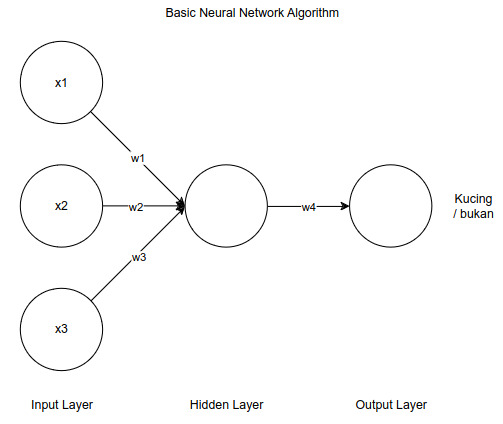
\includegraphics[scale=0.6]{gambar/bab2-basic-nn.jpeg}
  \caption{Diagram sederhana dari \emph{Neural Network}}
  \label{fig:basic_nn}
\end{figure}

\subsubsection{\emph{Perceptron}}
\emph{Perceptron} merupakan dasar dari NN, yang diperkenalkan oleh Frank Rosenblatt pada tahun 1958 \parencite*{rosenblatt1958perceptron}. \emph{Perceptron} adalah model jaringan saraf tiruan yang paling sederhana, yang memodelkan sebuah neuron dalam otak.

Struktur dasar \emph{perceptron} terdiri dari \emph{input} \( x_1, x_2, \dots, x_n \), \emph{weights} (bobot) \( w_1, w_2, \dots, w_n \), dan bias \( b \). \emph{Output} dari \emph{perceptron} dihitung menggunakan rumus:
\[ y = f(w \cdot x + b) \]
dimana \( f \) adalah fungsi aktivasi, \( w \cdot x \) adalah \emph{dot product} antara vektor bobot dan vektor input, dan \( b \) adalah bias.
 
 \subsubsection{\emph{Activation Function}}
 \emph{Activation function} menentukan \emph{output} dari sebuah \emph{neuron} berdasarkan \emph{input} total yang diterima. Beberapa fungsi aktivasi yang sering digunakan adalah:
 \begin{itemize}
   \item Sigmoid: \( \sigma(x) = \frac{1}{1 + e^{-x}} \). Fungsi ini menghasilkan \emph{output} dalam rentang \( (0, 1) \), yang berguna untuk tugas klasifikasi biner.
   \item Tanh: \( \tanh(x) = \frac{e^{x} - e^{-x}}{e^{x} + e^{-x}} \). Fungsi ini menghasilkan \emph{output} dalam rentang \( (-1, 1) \), yang membantu dalam mengatasi masalah \emph{vanishing gradient}. Yaitu ketika nilai \emph{input} yang besar atau kecil menyebabkan gradien yang sangat kecil.
   \item ReLU (Rectified Linear Unit): \( ReLU(x) = \max(0, x) \). Fungsi ini menghasilkan \emph{output} \( 0 \) jika \emph{input} \( x \leq 0 \) dan \( x \) jika \( x > 0 \). ReLU adalah fungsi aktivasi yang paling umum digunakan dalam arsitektur NN modern karena sederhana dan efektif.
 \end{itemize}

 Berikut beberapa grafik dari \emph{activation function} yang disebutkan di atas.

  \begin{figure}[H]
    \centering
    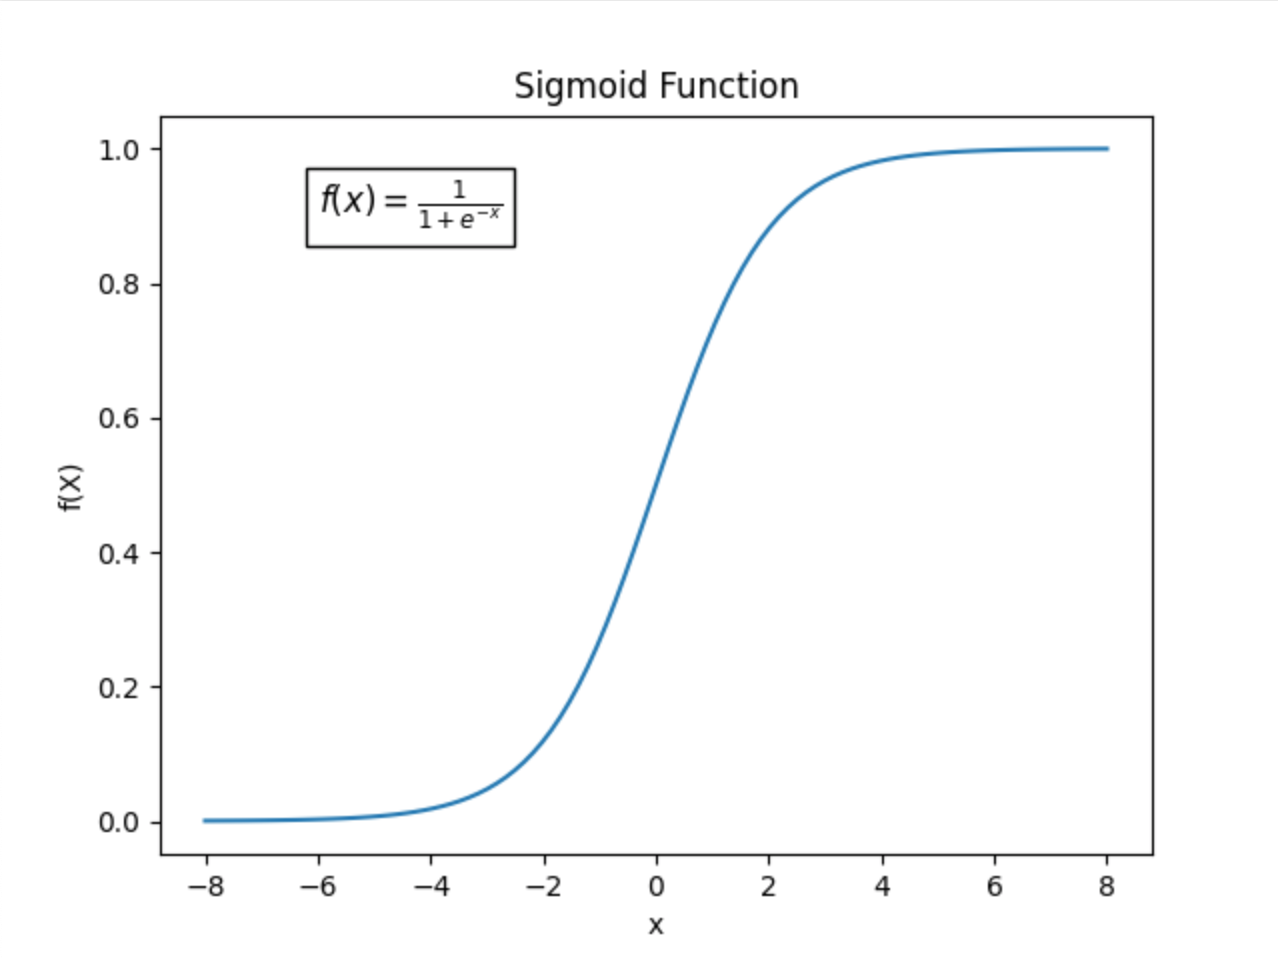
\includegraphics[scale=0.4]{gambar/bab2-grafik-sigmoid.png}
    \caption{Grafik \emph{Activation function Sigmoid}}
    \label{fig:sigmoid_function}
  \end{figure}

  \begin{figure}[H]
    \centering
    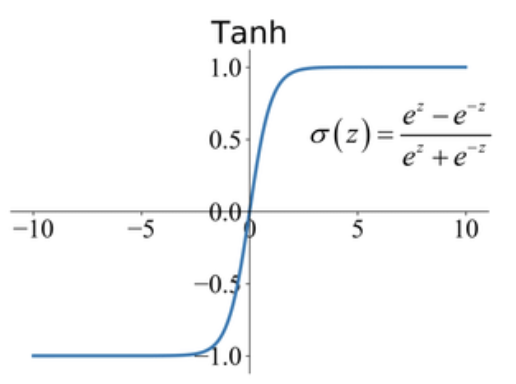
\includegraphics[scale=0.8]{gambar/bab2-grafik-tanh.png}
    \caption{Grafik \emph{Activation function Tanh}}
    \label{fig:tanh_function}
  \end{figure}

  \begin{figure}[H]
    \centering
    \includegraphics[scale=0.5]{gambar/bab2-grafik-relu.png}
    \caption{Grafik \emph{Activation function ReLU}}
    \label{fig:relu_function}
  \end{figure}
 
 \subsubsection{\emph{Feed Forward}}
 Mekanisme \emph{feed forward} adalah proses pengiriman input melalui lapisan-lapisan dari NN untuk mendapatkan \emph{output}. Setiap neuron dalam lapisan menerima \emph{input} dari semua neuron di lapisan sebelumnya, mengaplikasikan bobot dan bias, dan menghasilkan \emph{output} menggunakan fungsi aktivasi.
 
 \subsubsection{\emph{Backpropagation}}
 \emph{Backpropagation} adalah metode yang digunakan untuk memperbarui bobot jaringan dengan cara mengoptimalkan fungsi kerugian. Proses ini melibatkan penghitungan gradien fungsi kerugian terhadap setiap bobot di jaringan dengan menggunakan aturan rantai, dan secara iteratif mengatur ulang bobot untuk meminimalkan \emph{loss}.
 
 \begin{figure}[H]
  \centering
  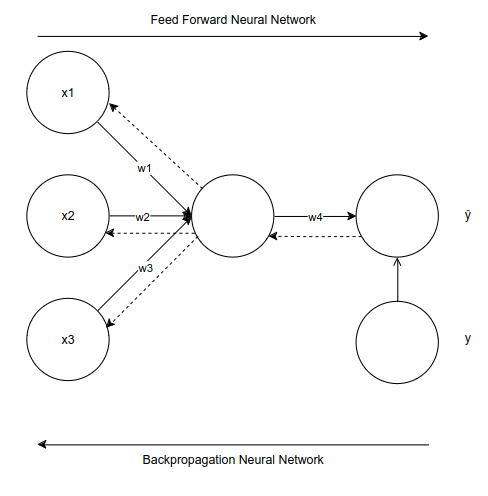
\includegraphics[scale=0.6]{gambar/bab2-ff-backprop.png}
  \caption{Perbedaan antara \emph{Feed Forward} dan \emph{Backpropagation}}
  \label{fig:ff_backprop}
\end{figure}

 \subsubsection{\emph{Loss Function} dan \emph{Optimizer}}
 \emph{Loss function} mengukur seberapa baik model NN melakukan prediksi dibandingkan dengan nilai sebenarnya. \emph{Loss function} yang umum meliputi:
 \begin{itemize}
   \item \textbf{\emph{Gradient Descent}}: Metode optimisasi yang digunakan untuk meminimalkan fungsi kerugian dengan mengupdate bobot jaringan berdasarkan gradien fungsi kerugian.
   \item \textbf{\emph{Stochastic Gradient Descent} (SGD)}: Versi sederhana dari \emph{Gradient Descent} yang memperbarui bobot jaringan berdasarkan gradien dari satu sampel data.
   \item \textbf{\emph{Momentum}}: Metode optimisasi yang membantu percepatan konvergensi dengan menambahkan momentum pada proses \emph{Gradient Descent}.
   \item \textbf{\emph{RMSprop}}: Metode optimisasi yang menyesuaikan laju pembelajaran untuk setiap parameter berdasarkan gradien rata-rata kuadrat sebelumnya.
   \item \textbf{\emph{Adam}}: Algoritma optimisasi yang menggabungkan konsep dari \emph{Momentum} dan \emph{RMSprop} untuk memperbarui bobot jaringan secara adaptif.
 \end{itemize}
 
 Optimisasi adalah proses mencari parameter model yang meminimalkan fungsi kerugian. Algoritma optimisasi yang sering digunakan antara lain \emph{Stochastic Gradient Descent} (SGD), \emph{Adam}, dan \emph{RMSprop}. Adapun pada penelitian ini, digunakan algoritma Adam sebagai \emph{optimizer} untuk memperbarui bobot jaringan karena kemampuannya dalam menyesuaikan laju pembelajaran secara adaptif.
 
 \subsubsection{CNN (\emph{Convolutional Neural Network})}
 CNN (\emph{Convolutional Neural Networks}) memperluas konsep NN dengan memasukkan lapisan konvolusi, yang menggunakan filter untuk mengekstraksi fitur spatial dari data \emph{input}. Berikut merupakan beberapa konsep dasar dalam CNN:
 \begin{itemize}
   \item \textbf{\emph{Convolutional Layer}}: Menggunakan filter atau \emph{kernel} yang 'meluncur' di atas gambar untuk menghasilkan \emph{feature map}.
   \item \textbf{\emph{Stride}}: Jumlah piksel yang dilewati filter pada setiap gerakan. Stride yang lebih besar menghasilkan \emph{feature map} yang lebih kecil.
   \item \textbf{\emph{Padding}}: Penambahan piksel di sekitar input untuk memungkinkan filter beroperasi di tepi gambar.
   \item \textbf{\emph{Pooling Layer}} (\emph{Subsampling}): Mengurangi dimensi spatial dari \emph{feature map} untuk mengurangi jumlah parameter dan komputasi. Contohnya adalah \emph{max pooling} dan \emph{average pooling}.
   \item \textbf{\emph{Fully Connected Layer}}: Lapisan di mana setiap neuron terhubung ke semua neuron di lapisan sebelumnya, biasanya digunakan di akhir jaringan untuk mengklasifikasikan fitur yang diekstraksi oleh lapisan konvolusi.
 \end{itemize} 

 CNN merupakan salah satu arsitektur \emph{deep learning} yang paling banyak digunakan dalam pengolahan citra. CNN pertama kali diperkenalkan oleh Yan LeCun et al. \parencite*{yannlecun1998} dalam penelitian tentang pengenalan tulisan tangan menggunakan LeNet-5. Model ini menggabungkan operasi konvolusi, \emph{subsampling} (\emph{pooling}), dan \emph{fully connected layers} untuk mengekstraksi fitur secara hierarkis dari gambar \emph{input}.
 
Perkembangan CNN semakin pesat dengan adanya inovasi pada arsitektur. Salah satu inovasi signifikan adalah \emph{Residual Neural Network} (ResNet) yang diperkenalkan oleh Kaiming He et al. \parencite*{kaiminghe2015}. ResNet memperkenalkan konsep \emph{skip connection} yang memungkinkan model untuk belajar representasi yang lebih baik dari data. Hal ini memungkinkan model untuk dilatih dengan kedalaman yang lebih besar tanpa mengalami masalah \emph{vanishing gradient}.
 
Selain itu, metode modern seperti normalisasi \emph{batch} (\emph{BatchNorm}) yang dikembangkan oleh Ioffe et al. \parencite*{ioffe2015} dan Szegedy et al. \parencite*{szegedy2015} telah menjadi standar dalam \emph{training} CNN. \emph{BatchNorm} membantu jaringan untuk melakukan konvergensi lebih cepat dengan menormalkan distribusi setiap \emph{batch} selama pelatihan. Penggunaan konvolusi 1x1, seperti pada arsitektur \emph{Inception}, juga memperkenalkan cara baru untuk mengurangi jumlah parameter sambil mempertahankan kapasitas jaringan.
 
Penerapan CNN telah meluas ke berbagai domain, termasuk deteksi objek, segmentasi citra, dan pengenalan pola. Dalam konteks penelitian ini, CNN digunakan untuk mendeteksi kendaraan overdimensi berdasarkan karakteristik visualnya. Pendekatan ini sesuai dengan studi sebelumnya yang menunjukkan kemampuan CNN dalam mengolah data visual dengan tingkat akurasi yang tinggi.
\subsection{SSD (\emph{Single Shot MultiBox Detector})}

\emph{Single Shot MultiBox Detector} (SSD) adalah arsitektur deteksi objek yang dikembangkan oleh Liu et al. \parencite*{liu2016}. SSD memperkenalkan pendekatan \emph{single shot} yang memungkinkan model untuk melakukan deteksi objek dan klasifikasi dalam satu langkah. Hal ini berbeda dengan pendekatan \emph{two-stage} seperti Faster R-CNN yang memerlukan dua tahap untuk deteksi objek.

SSD menggunakan \emph{multi-scale feature maps} untuk mendeteksi objek pada berbagai skala. Arsitektur ini terdiri dari \emph{base network} (biasanya menggunakan arsitektur VGG16 atau ResNet) yang diikuti oleh beberapa lapisan konvolusi untuk menghasilkan \emph{feature maps} pada berbagai resolusi. Setiap lapisan \emph{feature map} digunakan untuk memprediksi \emph{bounding box} dan kelas objek yang terdapat dalam gambar.

\begin{figure}[H]
  \centering
  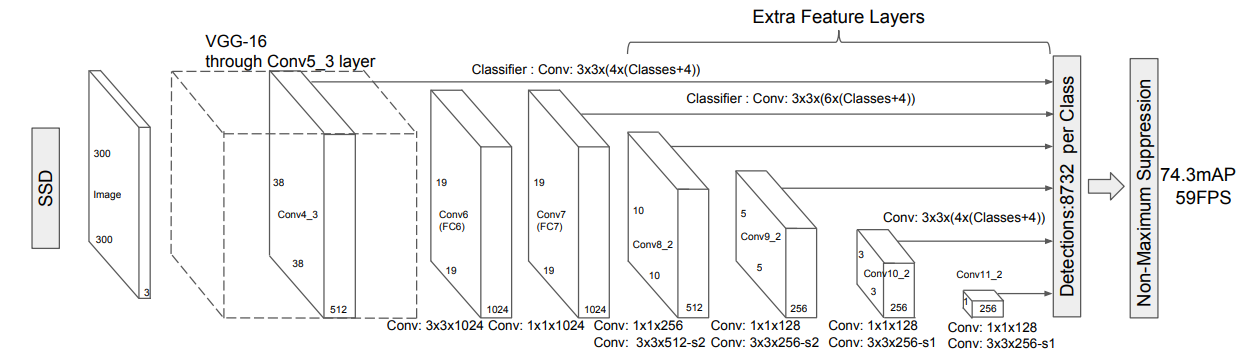
\includegraphics[scale=0.36]{gambar/bab2-arsitektur-ssd.png}
  \caption{Arsitektur SSD}
  \label{fig:arsitektur_ssd}
\end{figure}

SSD telah terbukti efektif dalam deteksi objek pada berbagai \emph{dataset}, termasuk PASCAL VOC dan COCO. Keunggulan utama SSD adalah kemampuannya untuk melakukan deteksi objek secara cepat dan akurat dalam satu langkah. Dalam penelitian ini, SSD digunakan sebagai model deteksi untuk mengidentifikasi kendaraan overdimensi pada video pengamatan jalan raya.

\subsection{\emph{Edge Computing}}

\emph{Edge computing} adalah paradigma komputasi yang memungkinkan pemrosesan data dilakukan di dekat sumber data, seperti perangkat \emph{IoT} (\emph{Internet of Things}) atau sensor. Hal ini bertentangan dengan komputasi tradisional yang memerlukan pengiriman data ke pusat data atau cloud untuk diproses. \emph{Edge computing} memungkinkan pemrosesan data yang lebih cepat, responsif, dan efisien dengan memanfaatkan sumber daya lokal.

Keuntungan utama dari \emph{edge computing} adalah kemampuannya untuk mengurangi latensi dan mempercepat respons sistem \parencite*{aws2024}. Dengan melakukan pemrosesan data di dekat sumber data, \emph{edge computing} memungkinkan aplikasi untuk merespons lebih cepat terhadap perubahan kondisi lingkungan. Hal ini sangat penting dalam konteks aplikasi \emph{real-time} seperti deteksi objek pada video pengamatan jalan raya.

Selain itu, \emph{edge computing} juga membantu mengurangi beban jaringan dan \emph{cloud} dengan melakukan pemrosesan data secara lokal. Hal ini dapat mengurangi biaya operasional dan meningkatkan efisiensi sistem secara keseluruhan. Dalam konteks penelitian ini, \emph{edge computing} digunakan untuk menjalankan model deteksi objek secara \emph{real-time} pada perangkat lokal tanpa memerlukan koneksi internet. 

Contoh implementasi edge computing yang digunakan dalam penelitian ini adalah Jetson Nano dan Beelink Gemini T34 yang berfungsi sebagai \emph{edge device} untuk menjalankan model deteksi objek secara \emph{real-time}.

\subsubsection{Jetson Nano}

 \begin{figure}[H]
  \centering
  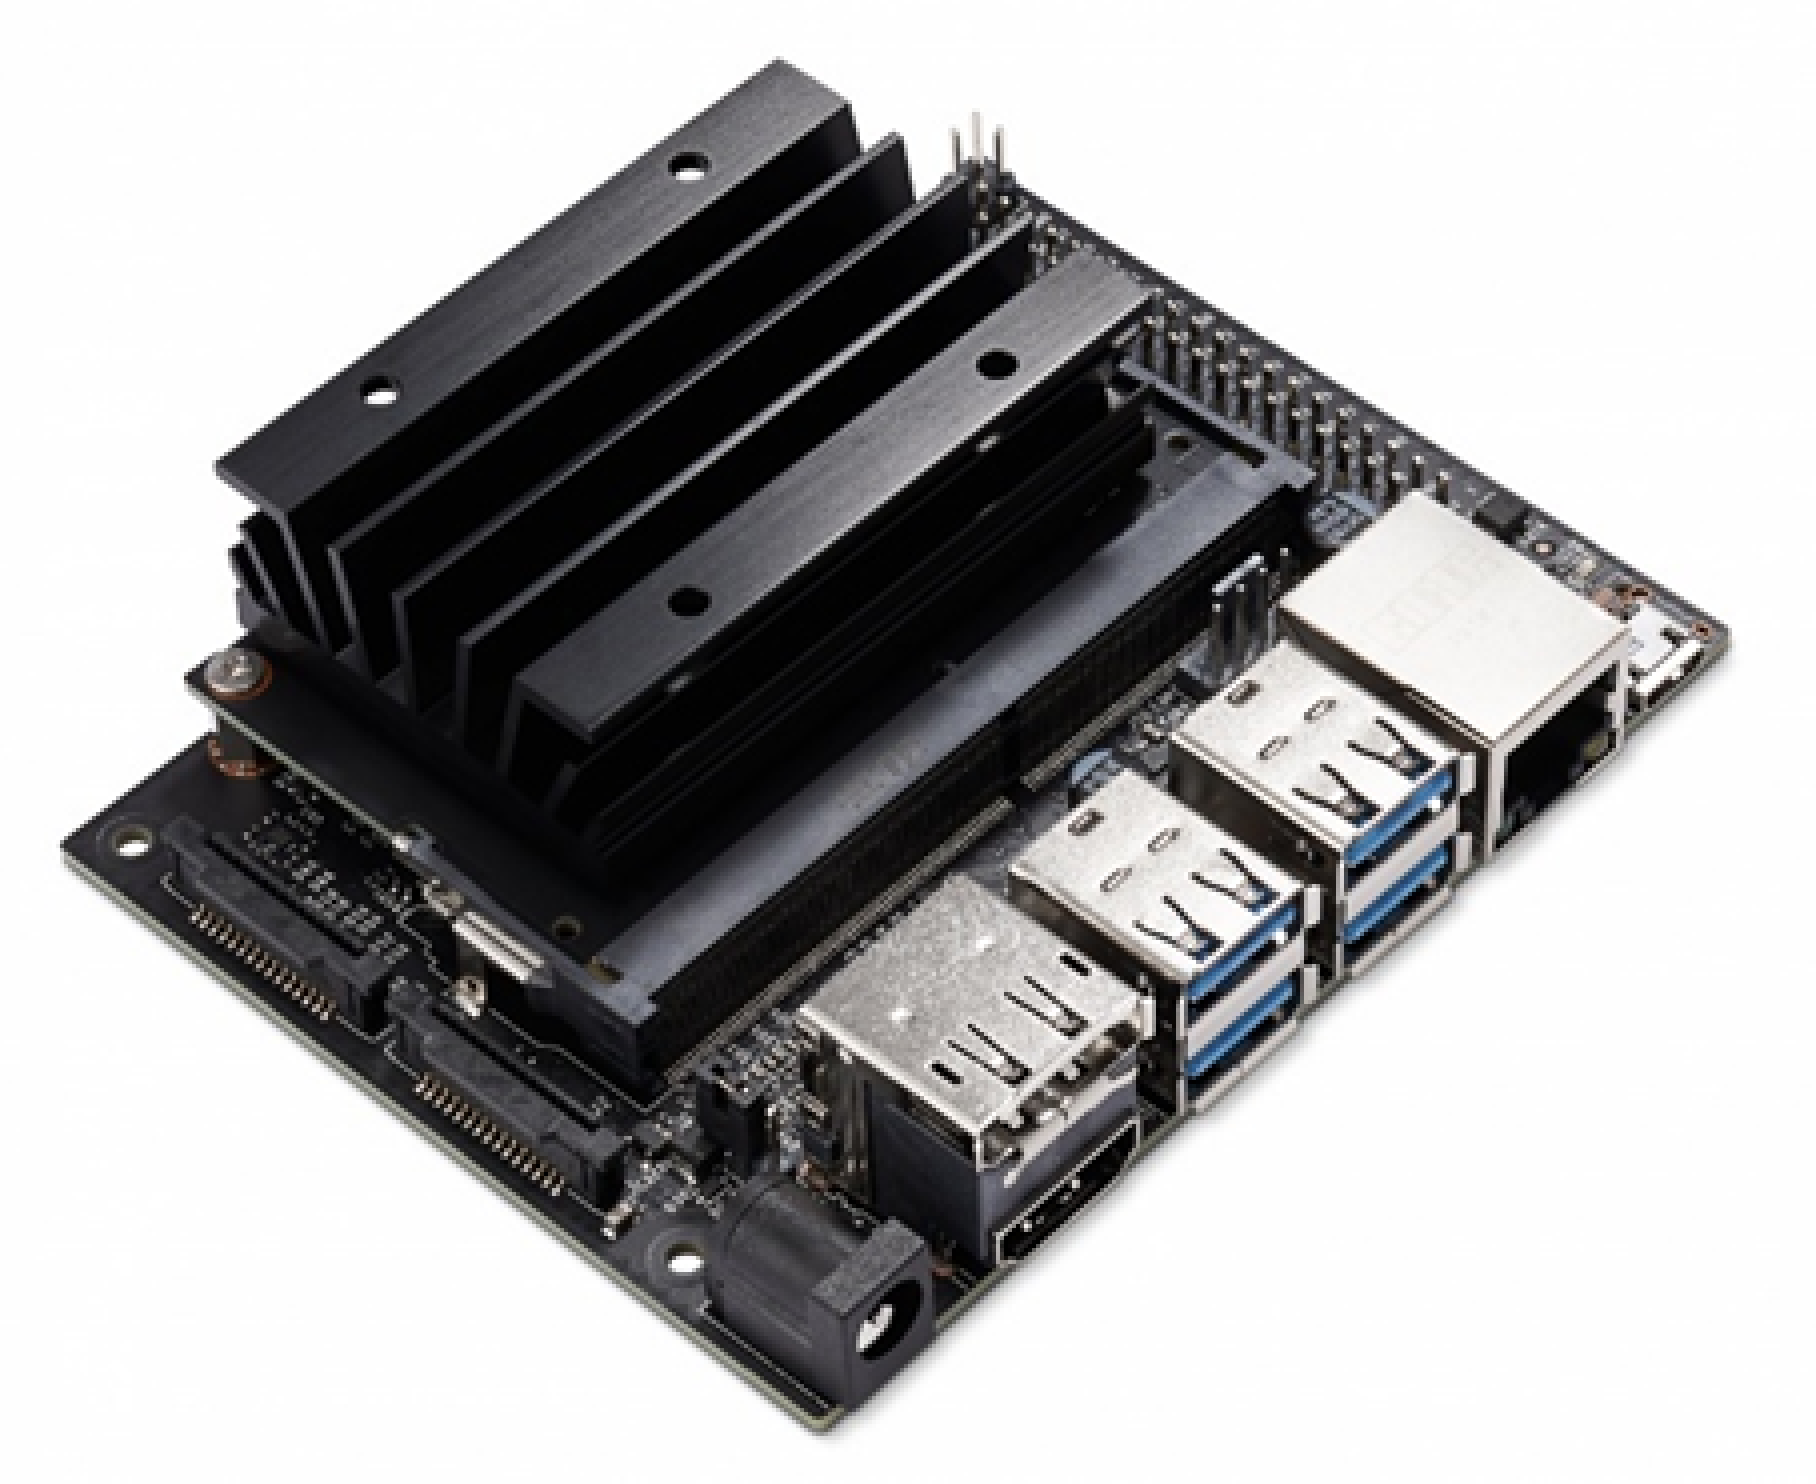
\includegraphics[scale=0.7]{gambar/bab2-jetson-nano.png}
  \caption{Jetson Nano Developer Kit}
  \label{fig:jetsonnano}
\end{figure}

Jetson Nano adalah perangkat komputasi keluaran NVIDIA yang didedikasikan dalam pengembangan \textit{machine learning} dan \emph{edge computing}. Jetson Nano memiliki kemampuan untuk dapat menjalankan beberapa \emph{neural networks} secara paralel. Kemampuan ini memungkinkan Jetson Nano untuk digunakan dalam \textit{image classification}, \textit{object detection}, \textit{segmentation}, dan \textit{speech processing} \parencite{nvidiaJetsonNano}. Perangkat ini dapat menjadi solusi dalam menjalankan model \textit{machine learning} atau \textit{deep learning} pada perangkat portable dan hemat energi. 

Perangkat ini dilengkapi dengan 128 NVIDIA CUDA \emph{cores}. Ditenagai oleh prosesor \emph{Quad-core ARM Cortex-A57 MPCore}, platform ini menyediakan fungsionalitas komputasi yang solid dengan memori 4 GB 64-bit LPDDR4 yang beroperasi pada 1600MHz, memberikan \emph{bandwidth} 25.6 GB/s. Untuk penyimpanan, Jetson Nano dilengkapi dengan 16 GB eMMC 5.1, yang memberikan ruang yang cukup untuk aplikasi dan data pengguna. Jetson Nano dapat mengkodekan video dengan kecepatan 250MP/sec, mendukung format seperti 1x 4K pada 30fps (HEVC), 2x 1080p pada 60fps (HEVC), dan sebagainya. Sementara itu, untuk decode video, perangkat ini menawarkan kemampuan hingga 500MP/sec, dengan dukungan untuk format seperti 1x 4K pada 60fps (HEVC) dan 2x 4K pada 30fps (HEVC). Jetson Nano juga dilengkapi dengan 12 jalur kamera (3x4 atau 4x2) MIPI CSI-2 D-PHY 1.1, yang mendukung kecepatan hingga 1.5 Gb/s per pasangan, memberikan fleksibilitas dalam pengembangan aplikasi berbasis kamera. Dalam hal konektivitas, perangkat ini menawarkan Gigabit Ethernet dan M.2 Key E, serta kemampuan tampilan melalui HDMI 2.0 dan eDP 1.4. Jetson Nano juga dilengkapi dengan 4x USB 3.0 dan USB 2.0 Micro-B, serta berbagai opsi konektivitas lainnya seperti GPIO, I2C, I2S, SPI, dan UART, semuanya dalam form factor mekanis 69.6 mm x 45 mm dengan konektor tepi 260-pin \parencite{nvidiaJetsonNano}.

\subsubsection{Beelink Gemini T34}
 \begin{figure}[H]
     \centering
     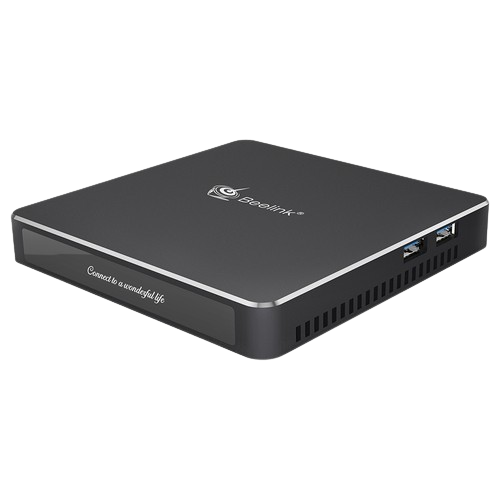
\includegraphics[scale=0.6]{gambar/bab2-beelink-gemini-t34.png}
     \caption{Beelink Gemini T34}
     \label{fig:beelinkgeminit34}
\end{figure}

Beelink Gemini T34 adalah mini PC yang dilengkapi dengan prosesor Intel Apollo Lake N3450. Prosesor ini memiliki 4 core dan 4 thread dengan kecepatan hingga 2.2 GHz. Beelink Gemini T34 juga dilengkapi dengan Intel HD Graphics 500 yang mendukung resolusi hingga 4K. Mini PC ini memiliki RAM 8 GB LPDDR3 dan penyimpanan 128 GB eMMC SSD. Beelink Gemini T34 memiliki berbagai port konektivitas seperti HDMI, USB 3.0, USB 2.0, dan Gigabit Ethernet. Mini PC ini juga dilengkapi dengan konektivitas Wi-Fi 5 dan Bluetooth 4.0. Beelink Gemini T34 memiliki dimensi 11.9 cm x 11.9 cm x 1.79 cm dan berat 0.4 kg, sehingga mudah dipindahkan dan ditempatkan di berbagai lokasi. \parencite*{beelinkGeminiT34}

Beelink Gemini T34 dapat digunakan sebagai \emph{edge device} untuk menjalankan model deteksi objek secara \emph{real-time}. Mini PC ini memiliki performa yang cukup untuk menjalankan aplikasi deteksi objek dengan akurasi tinggi dan latensi rendah. Dengan konektivitas Wi-Fi dan Bluetooth, Beelink Gemini T34 dapat terhubung ke jaringan lokal dan perangkat lain untuk mentransfer data deteksi objek. Dengan demikian, Beelink Gemini T34 merupakan solusi yang ideal untuk implementasi \emph{edge computing} dalam deteksi objek pada video pengamatan jalan raya.

% \subsection{MQTT (\emph{Message Queuing Telemetry Transport})}

% MQTT (\emph{Message Queuing Telemetry Transport}) adalah protokol komunikasi yang ringan dan efisien untuk pertukaran pesan antara perangkat. MQTT dirancang untuk digunakan dalam kondisi jaringan yang tidak stabil atau berkapasitas rendah, seperti pada perangkat IoT atau \emph{edge device}.

% MQTT menggunakan model \emph{publish-subscribe} yang memungkinkan perangkat untuk berkomunikasi secara asinkron. Dalam model ini, perangkat yang mengirim pesan disebut \emph{publisher}, sedangkan perangkat yang menerima pesan disebut \emph{subscriber}. Pesan dikirim ke topik tertentu dan dapat diterima oleh satu atau lebih \emph{subscriber} yang berlangganan topik tersebut.

% Keunggulan utama dari MQTT adalah kemampuannya untuk mengirim pesan secara efisien dan andal di berbagai kondisi jaringan. MQTT menggunakan protokol TCP/IP yang ringan dan memiliki overhead yang rendah, sehingga cocok untuk digunakan pada perangkat dengan sumber daya terbatas. Selain itu, MQTT juga mendukung koneksi yang tahan lama dan \emph{quality of service} (QoS) yang dapat disesuaikan.

% Dalam penelitian ini, MQTT digunakan sebagai protokol komunikasi antara \emph{edge device} dan \emph{cloud} untuk mentransfer data deteksi objek secara \emph{real-time}. MQTT memungkinkan perangkat untuk berkomunikasi secara efisien dan responsif tanpa memerlukan koneksi internet yang stabil. \parencite*{mqtts2008}

\subsection{RESTful API}

RESTful API (\emph{Representational State Transfer Application Programming Interface}) adalah arsitektur desain yang digunakan untuk membangun layanan web yang ringan, fleksibel, dan mudah diakses. RESTful API menggunakan prinsip REST yang memisahkan antara data dan tampilan, serta memanfaatkan metode HTTP untuk berkomunikasi antara klien dan server.

RESTful API menggunakan 4 metode HTTP utama untuk berinteraksi dengan \emph{resource}:
\begin{itemize}[nolistsep]
  \item \textbf{GET}: Mengambil data dari \emph{resource}.
  \item \textbf{POST}: Membuat data baru di \emph{resource}.
  \item \textbf{PUT}: Memperbarui data yang ada di \emph{resource}.
  \item \textbf{DELETE}: Menghapus data dari \emph{resource}.
\end{itemize}

RESTful API menggunakan URI (\emph{Uniform Resource Identifier}) untuk mengidentifikasi sumber daya yang diakses dan format data yang diinginkan. Data dikirimkan dalam format yang umum seperti JSON atau XML untuk memudahkan pertukaran data antara klien dan server. \parencite*{restapi2016}

Keunggulan utama dari RESTful API adalah kemudahan penggunaan, fleksibilitas, dan skalabilitas. RESTful API memungkinkan pengembang untuk membangun layanan web yang dapat diakses dari berbagai platform dan bahasa pemrograman. Dalam penelitian ini, RESTful API digunakan untuk mengintegrasikan antara aplikasi Flutter dengan \emph{cloud} untuk mentransfer data deteksi objek secara \emph{real-time}.

\subsection{Flutter}

Flutter adalah \emph{framework} pengembangan aplikasi \emph{open-source} yang dikembangkan oleh \emph{Google} \parencite*{google2024}. Flutter memungkinkan pengembang untuk membuat aplikasi \emph{mobile} dengan antarmuka pengguna yang kaya dan responsif. Flutter menggunakan bahasa pemrograman Dart yang dikembangkan oleh Google sebagai bahasa utamanya.

Keunggulan utama dari Flutter adalah kemampuannya untuk membuat aplikasi \emph{mobile} yang konsisten di berbagai platform, termasuk Android dan iOS. Flutter menggunakan \emph{widget} sebagai komponen dasar untuk membangun antarmuka pengguna. \emph{Widget} Flutter bersifat deklaratif, yang berarti pengembang mendefinisikan bagaimana antarmuka pengguna harus terlihat berdasarkan kondisi saat ini.

Flutter juga menyediakan berbagai \emph{plugin} dan \emph{package} yang memperluas fungsionalitas aplikasi. Pengembang dapat menggunakan \emph{plugin} Flutter untuk mengakses fitur perangkat seperti kamera, lokasi, dan sensor. Selain itu, Flutter juga menyediakan \emph{package} untuk mengintegrasikan aplikasi dengan layanan \emph{cloud}, \emph{database}, dan API eksternal.

Dalam penelitian ini, Flutter digunakan sebagai platform pengembangan aplikasi \emph{mobile} untuk menampilkan hasil deteksi objek secara \emph{real-time}. Aplikasi Flutter akan berkomunikasi dengan \emph{cloud} untuk menerima data deteksi objek dan menampilkannya dalam antarmuka pengguna yang responsif.

\subsection{PostgreSQL}

PostgreSQL adalah sistem manajemen basis data relasional (\emph{RDBMS}) yang bersifat \emph{open-source} dan dapat diandalkan. PostgreSQL dikembangkan oleh komunitas pengembang yang aktif dan memiliki fitur yang lengkap untuk mengelola data dalam skala besar. PostgreSQL menggunakan bahasa SQL (\emph{Structured Query Language}) untuk berinteraksi dengan basis data dan mendukung berbagai jenis data dan operasi. \parencite*{postgresql2025}

Keunggulan utama dari PostgreSQL adalah keandalan, fleksibilitas, dan skalabilitas. PostgreSQL memiliki fitur transaksi ACID (\emph{Atomicity, Consistency, Isolation, Durability}) yang memastikan konsistensi data dan keandalan operasi. PostgreSQL juga mendukung berbagai jenis data seperti teks, angka, geometri, dan JSON, serta operasi kompleks seperti \emph{join}, \emph{subquery}, dan \emph{trigger}.

PostgreSQL juga memiliki dukungan yang baik untuk pengelolaan data dalam skala besar. PostgreSQL mendukung indeks, partisi, dan \emph{replication} untuk meningkatkan kinerja dan ketersediaan sistem. Selain itu, PostgreSQL juga memiliki fitur keamanan yang kuat seperti autentikasi, otorisasi, dan enkripsi data.

Dalam penelitian ini, PostgreSQL digunakan sebagai basis data untuk menyimpan data deteksi objek dan data pengguna. PostgreSQL akan digunakan untuk menyimpan informasi tentang objek yang terdeteksi, lokasi deteksi, dan waktu deteksi. Basis data ini akan digunakan oleh aplikasi Flutter untuk menampilkan data deteksi objek dan memungkinkan pengguna untuk melihat riwayat deteksi objek.

\subsection{Express.js}

Express.js adalah kerangka kerja web \emph{back-end} untuk Node.js yang minimalis dan fleksibel. Express.js menyediakan serangkaian fitur untuk membangun aplikasi web dan API dengan cepat dan mudah. Express.js menggunakan pendekatan \emph{middleware} yang memungkinkan pengembang untuk menambahkan fungsionalitas secara modular ke dalam aplikasi. \parencite*{expressjs2024}

Keunggulan utama Express.js meliputi:
\begin{itemize}[nolistsep]
  \item \textbf{Minimalis dan Fleksibel}: Express.js menyediakan fitur dasar yang diperlukan untuk membangun aplikasi web tanpa memaksakan struktur atau konvensi tertentu.
  \item \textbf{\emph{Middleware}}: Sistem \emph{middleware} memungkinkan pengembang untuk menambahkan fungsionalitas seperti \emph{logging}, autentikasi, dan penanganan kesalahan secara modular.
  \item \textbf{\emph{Routing}}: Express.js menyediakan sistem \emph{routing} yang kuat untuk menangani permintaan HTTP dengan berbagai metode dan parameter.
  \item \textbf{\emph{Template Engine}}: Mendukung berbagai \emph{template engine} untuk menghasilkan tampilan HTML dinamis.
\end{itemize}

\subsection{Apache HTTP Server}

Apache HTTP Server (Apache2) adalah server web \emph{open-source} yang paling banyak digunakan di dunia. Apache2 dikembangkan dan dikelola oleh Apache Software Foundation dan mendukung berbagai platform sistem operasi. Server ini dikenal karena kehandalannya, fleksibilitas konfigurasi, dan ekosistem modul yang luas. \parencite*{apache2024}

Fitur utama Apache2 meliputi:
\begin{itemize}[nolistsep]
  \item \textbf{\emph{Virtual Hosting}}: Kemampuan untuk menjalankan beberapa situs web pada satu server.
  \item \textbf{Modul Dinamis}: Mendukung penambahan dan penghapusan modul tanpa mengompilasi ulang server.
  \item \textbf{Keamanan}: Menyediakan fitur keamanan seperti SSL/TLS, autentikasi, dan otorisasi.
  \item \textbf{\emph{Reverse Proxy}}: Dapat berfungsi sebagai \emph{reverse proxy} untuk mendistribusikan beban dan meningkatkan keamanan.
\end{itemize}

\subsection{PM2 (Process Manager 2)}

PM2 adalah manajer proses untuk aplikasi Node.js yang memungkinkan pengembang untuk mengelola dan mempertahankan aplikasi tetap berjalan di lingkungan produksi. PM2 menyediakan fitur-fitur penting seperti load balancing, monitoring, dan manajemen log untuk memastikan ketersediaan dan kinerja aplikasi. \parencite*{pm22024}

Keunggulan utama PM2 meliputi:
\begin{itemize}[nolistsep]
  \item \textbf{\emph{Process Management}}: Kemampuan untuk menjalankan aplikasi dalam mode daemon, restart otomatis saat crash, dan update tanpa downtime.
  \item \textbf{\emph{Load Balancing}}: Mendistribusikan beban di antara beberapa instance aplikasi untuk meningkatkan throughput.
  \item \textbf{\emph{Monitoring}}: Menyediakan dashboard untuk memantau penggunaan CPU, memori, dan metrik lainnya secara real-time.
  \item \textbf{\emph{Log Management}}: Mengelola dan merotasi file log untuk mencegah penggunaan disk yang berlebihan.
\end{itemize}

\cleardoublepage

% Bab 3 desain dan implementasi
\chapter{METODOLOGI}
\label{chap:metodologi}

% Ubah bagian-bagian berikut dengan isi dari metodologi penelitian.

Dalam bab ini, akan dijelaskan metode yang digunakan dalam penelitian ini. Metode yang digunakan meliputi tahapan-tahapan yang dilakukan dalam penelitian ini, seperti pengumpulan data, analisis data, dan pengolahan data. Penjelasan ini akan membantu dalam memahami proses penelitian yang dilakukan.

\section{Blok Diagram}

\begin{figure}[htbp]
  \centering

  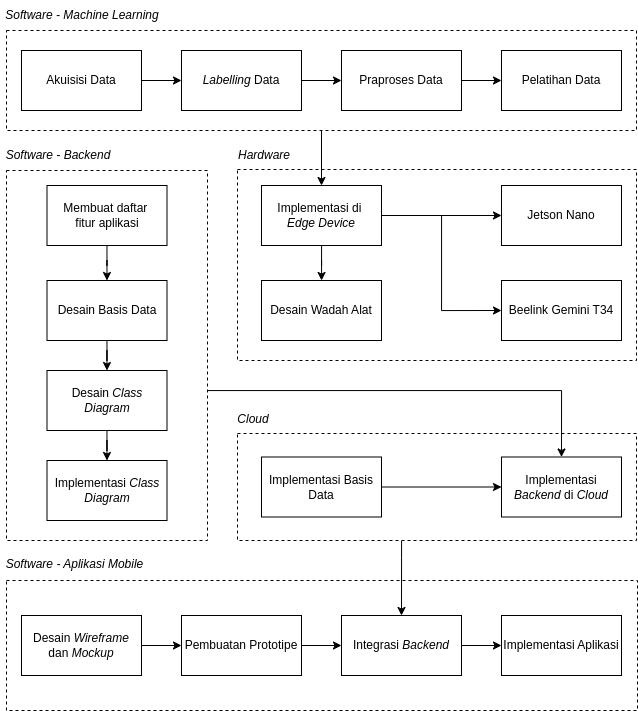
\includegraphics[scale=0.55]{gambar/bab3-block-diagram.png}

  \caption{Blok Diagram Sistem Deteksi Kendaraan Overdimension}
  \label{fig:blockdiagrammethod}
\end{figure}

Pada Gambar \ref{fig:blockdiagrammethod}, terdapat blok diagram yang menjelaskan bagian-bagian pengembangan sistem deteksi kendaraan \emph{overdimension} yang terbagi menjadi 3 bagian utama, yaitu \emph{software}, \emph{cloud}, \emph{hardware}. Lalu bagian \emph{software} sendiri terbagi menjadi 3 bagian, yaitu \emph{machine learning}, \emph{backend}, dan aplikasi \emph{mobile}. Berikut adalah penjelasan dari masing-masing bagian blok diagram:

\subsection{\emph{Software - Machine Learning}}
Pada bagian ini, dilakukan beberapa tahapan, yaitu:
\begin{enumerate}[nolistsep]
  \item Akuisisi data
  \item \emph{Labelling} data
  \item Praproses data
  \item Pelatihan data
\end{enumerate}

\textbf{Akuisisi data} dilakukan dengan mengambil data video dari kendaraan yang melintas. Akuisisi data dilakukan sebanyak 2 kali, yaitu di Jalan Tanjung Perak dan di Gerbang Tol Dupak 1 dan Dupak 2 setelah memperoleh izin ke Dinas Perhubungan selaku pihak yang menangani pelanggaran \emph{overdimension} dan PT. Jasa Marga selaku pengelola jalan tol. Data video yang diambil nantinya akan dipotong-potong menjadi beberapa frame. Frame-frame tersebut akan digunakan sebagai data latih untuk model \emph{machine learning} setelah melewati proses \emph{Labelling}. Gambar \ref{fig:acquisitiondata} menunjukkan proses akuisisi data yang telah dilakukan.

\begin{figure}[htbp]
  \centering

  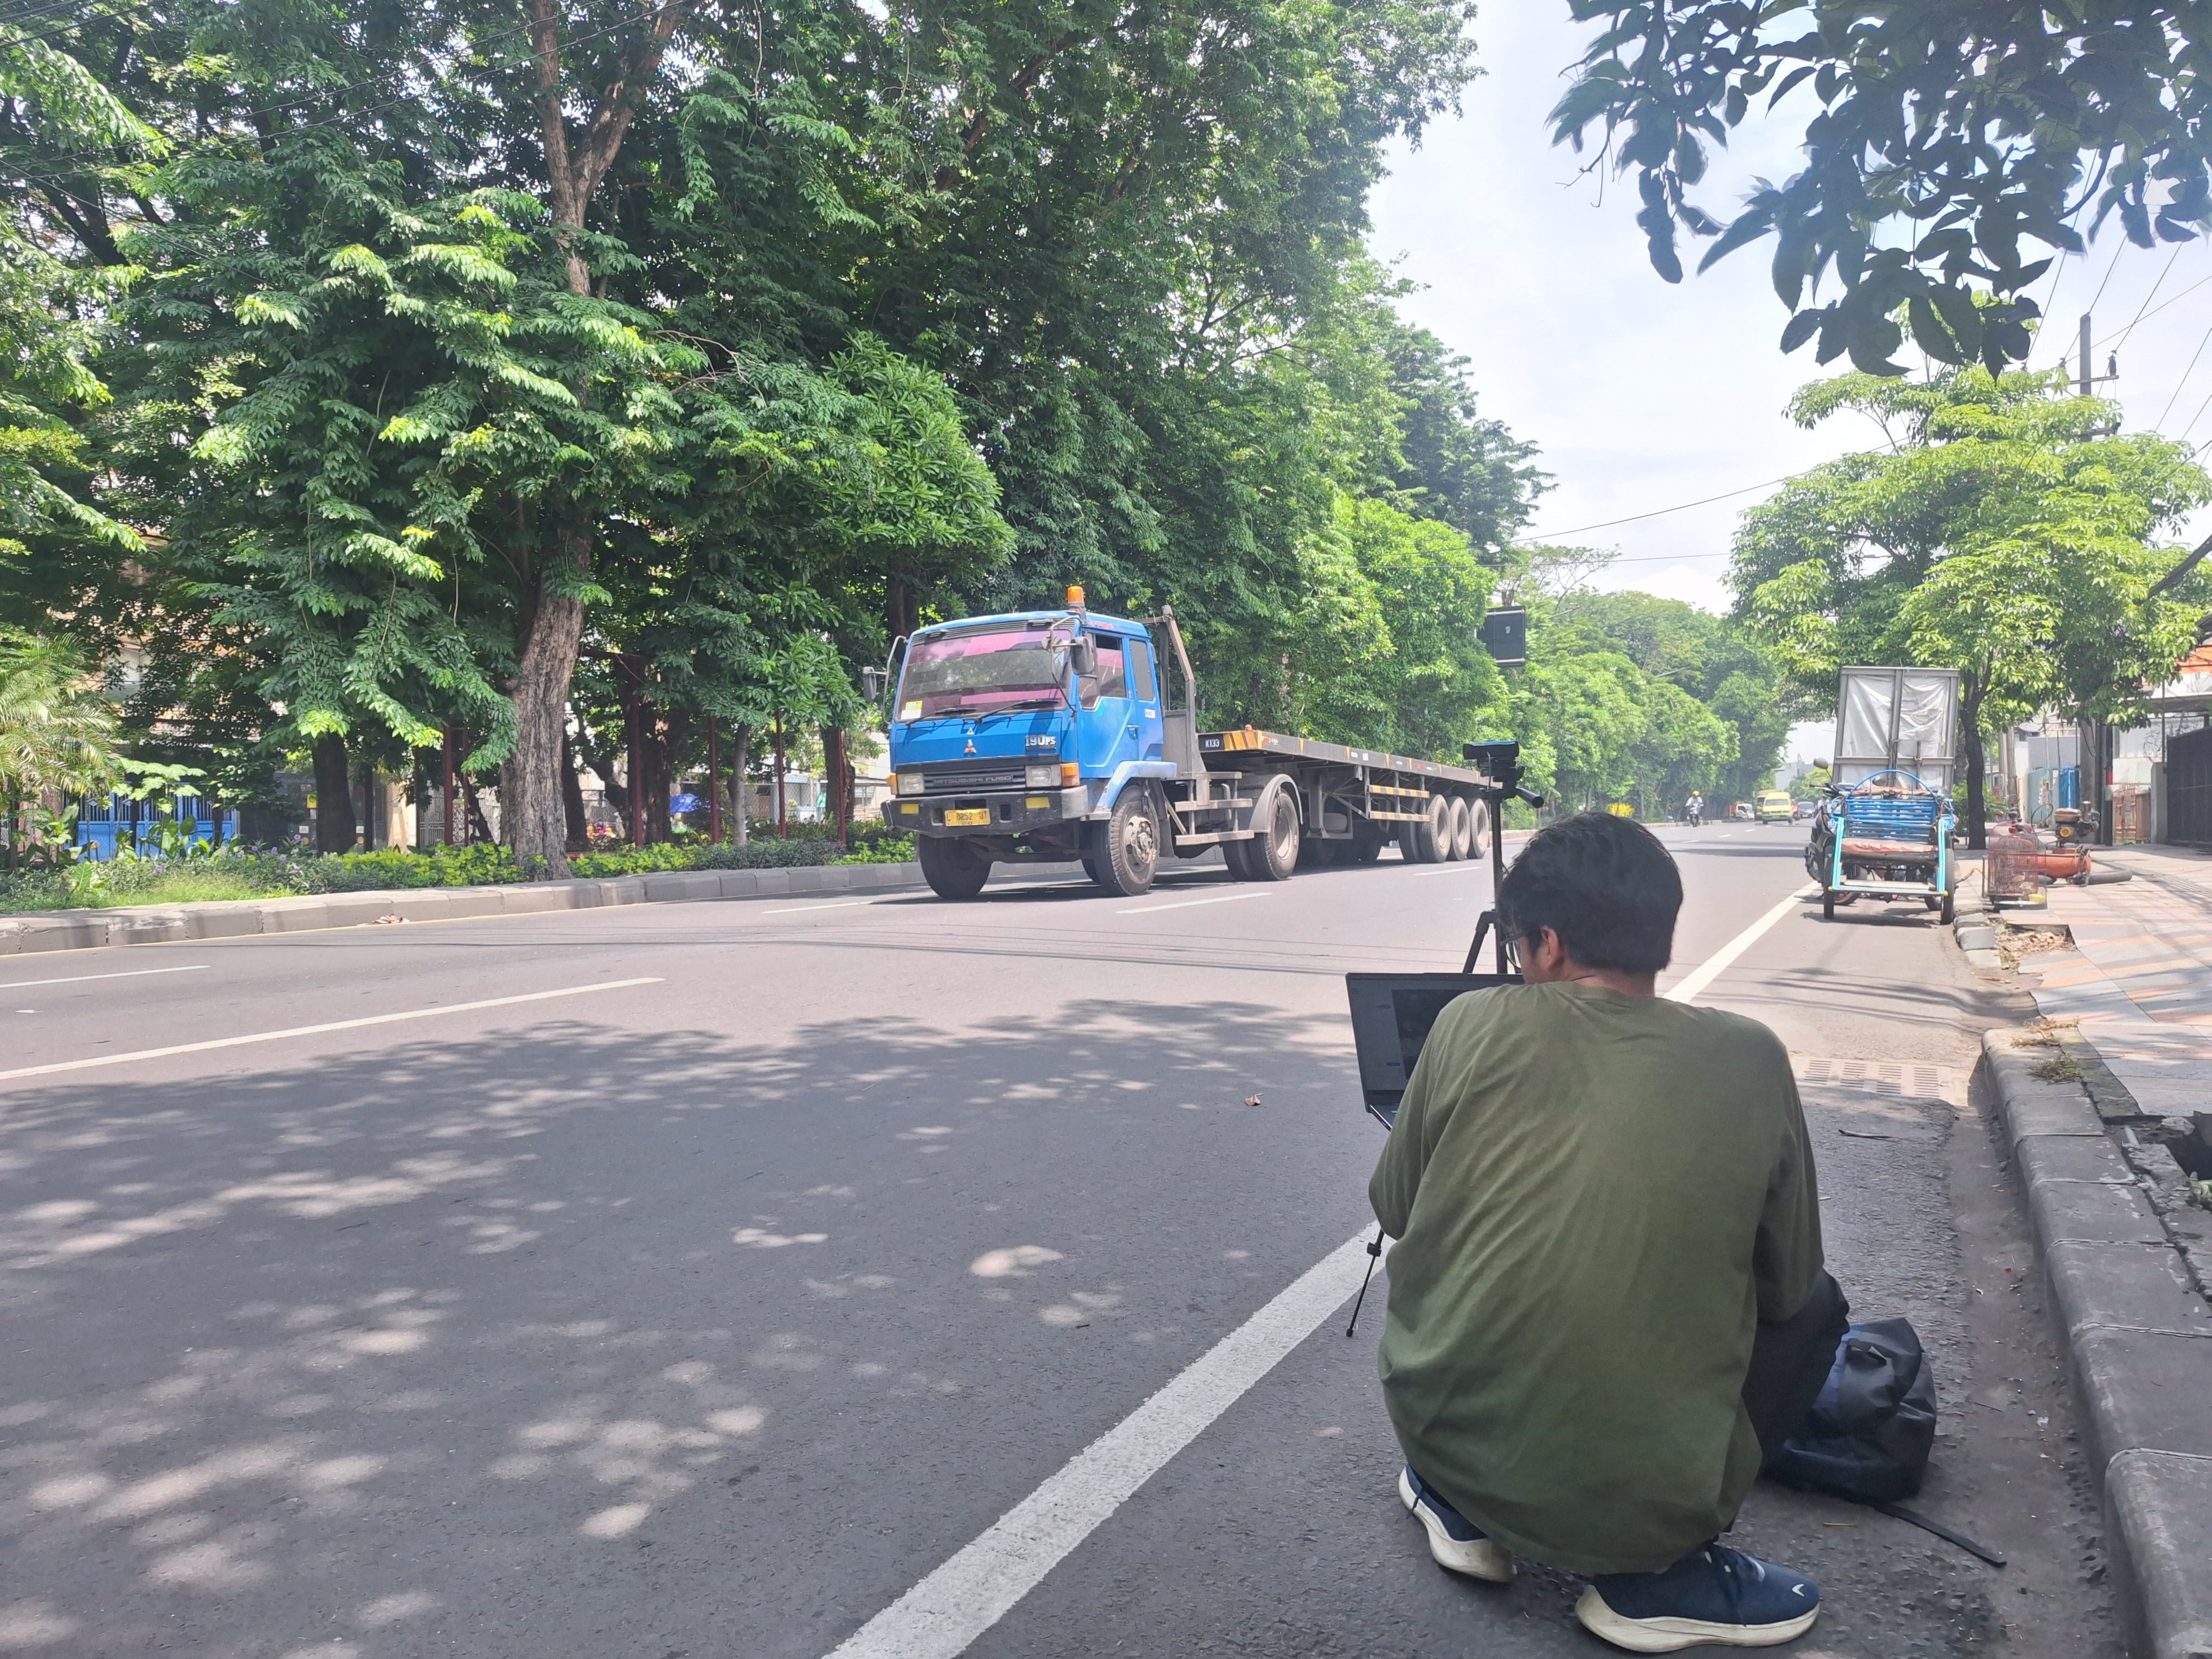
\includegraphics[scale=0.07]{gambar/bab3-acquisition-data.png}

  \caption{Proses Akuisisi Data di Jalan Tj. Perak Surabaya}
  \label{fig:acquisitiondata}
\end{figure}

Algoritma \emph{pseudocode} untuk pemotongan video menjadi frame dapat dilihat pada Algoritma \ref{alg:pemotonganvideomenjadiframe}.

\begin{algorithm}
  \caption{Pemotongan Video Menjadi Frame}
  \label{alg:pemotonganvideomenjadiframe}
  \begin{algorithmic}[1]
    \State \textbf{Input:} Video
    \State \textbf{Output:} Frame
    \State \textbf{Procedure:}
    \State \hspace{0.5cm} \textbf{while} \textit{video} \textbf{is playing}:
    \State \hspace{1cm} \textbf{if} \textit{space key pressed}:
    \State \hspace{1.5cm} \textit{frame} = \textit{video}.read
    \State \hspace{1.5cm} \textit{frame}.save(\textit{path})
    \State \hspace{0.5cm} \textbf{end while}
  \end{algorithmic}
\end{algorithm}

\textbf{\emph{Labelling} data} dilakukan dengan memberikan label pada data yang telah diakuisisi. Label yang diberikan adalah jenis kendaraan yang melintas dan apakah kendaraan tersebut termasuk \emph{overdimension} atau tidak. Proses \emph{labelling} ini dilakukan dengan menggunakan aplikasi \emph{Roboflow}. Gambar \ref{fig:labellingdata} menunjukkan proses \emph{labelling} data yang telah dilakukan.

\begin{figure}[h]
  \centering

  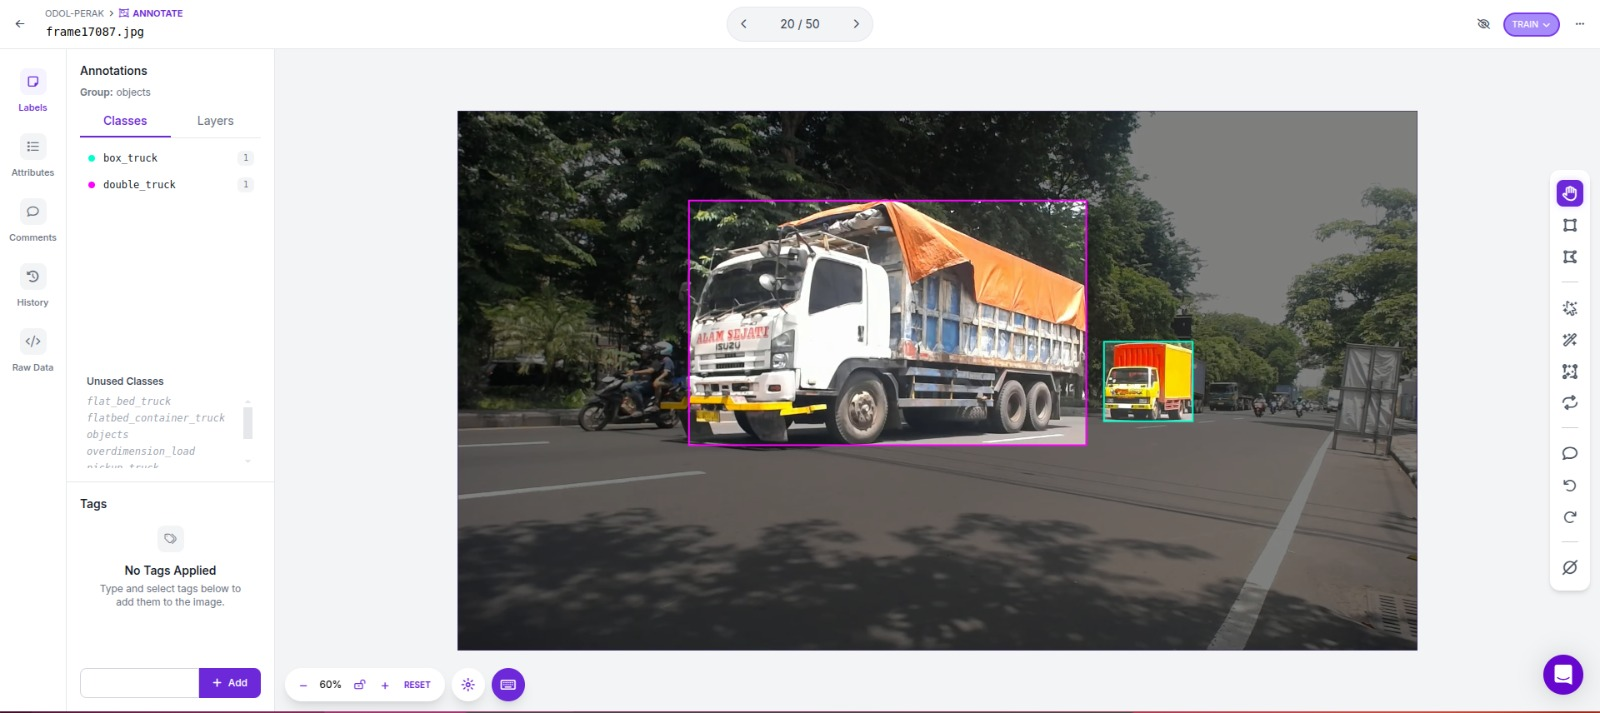
\includegraphics[scale=0.25]{gambar/bab3-labelling-data-nonoverdimension.jpeg}
  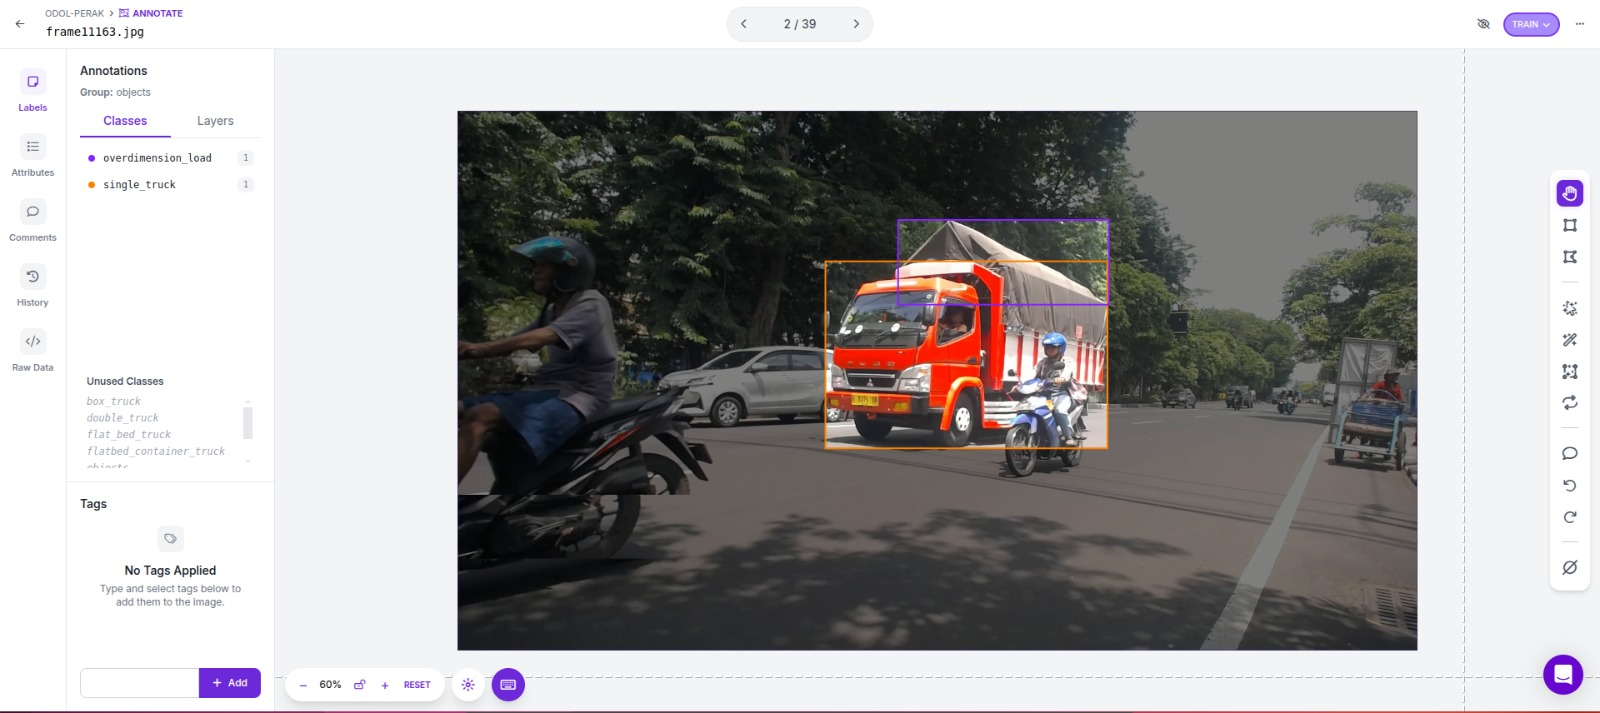
\includegraphics[scale=0.25]{gambar/bab3-labelling-data-overdimension.jpeg}

  \caption{\centering Proses \emph{Labelling} data menggunakan aplikasi \emph{Roboflow}, (atas) Kendaraan Non-\emph{Overdimension}, (bawah) Kendaraan \emph{Overdimension}}
  \label{fig:labellingdata}
\end{figure}

\textbf{Praproses data} dilakukan setelah data telah diberi label. Hal ini bertujuan untuk mempersiapkan data yang akan digunakan sebagai data latih pada model \emph{machine learning} dalam hal ini SSD-MobileNet-V2. Pada awalnya data yang telah diberi label akan disesuaikan orientasinya dan di-\emph{resize} ke ukuran 300x300 piksel. Kemudian dilakukan juga augmentasi data dengan cara memberikan \emph{brightness} (kecerahan) sebanyak -12\% hingga 12\% dan \emph{exposure} (paparan) sebanyak -10\% hingga 10\%.

Setelah itu, data akan dibagi menjadi data latih dan data validasi dengan perbandingan 80:20. Gambar \ref{fig:citraasli} menunjukkan citra asli yang akan dipraproses, sedangkan Gambar \ref{fig:preprocessingdata} menunjukkan proses praproses data yang telah dilakukan.

\begin{figure}[h]
  \centering

  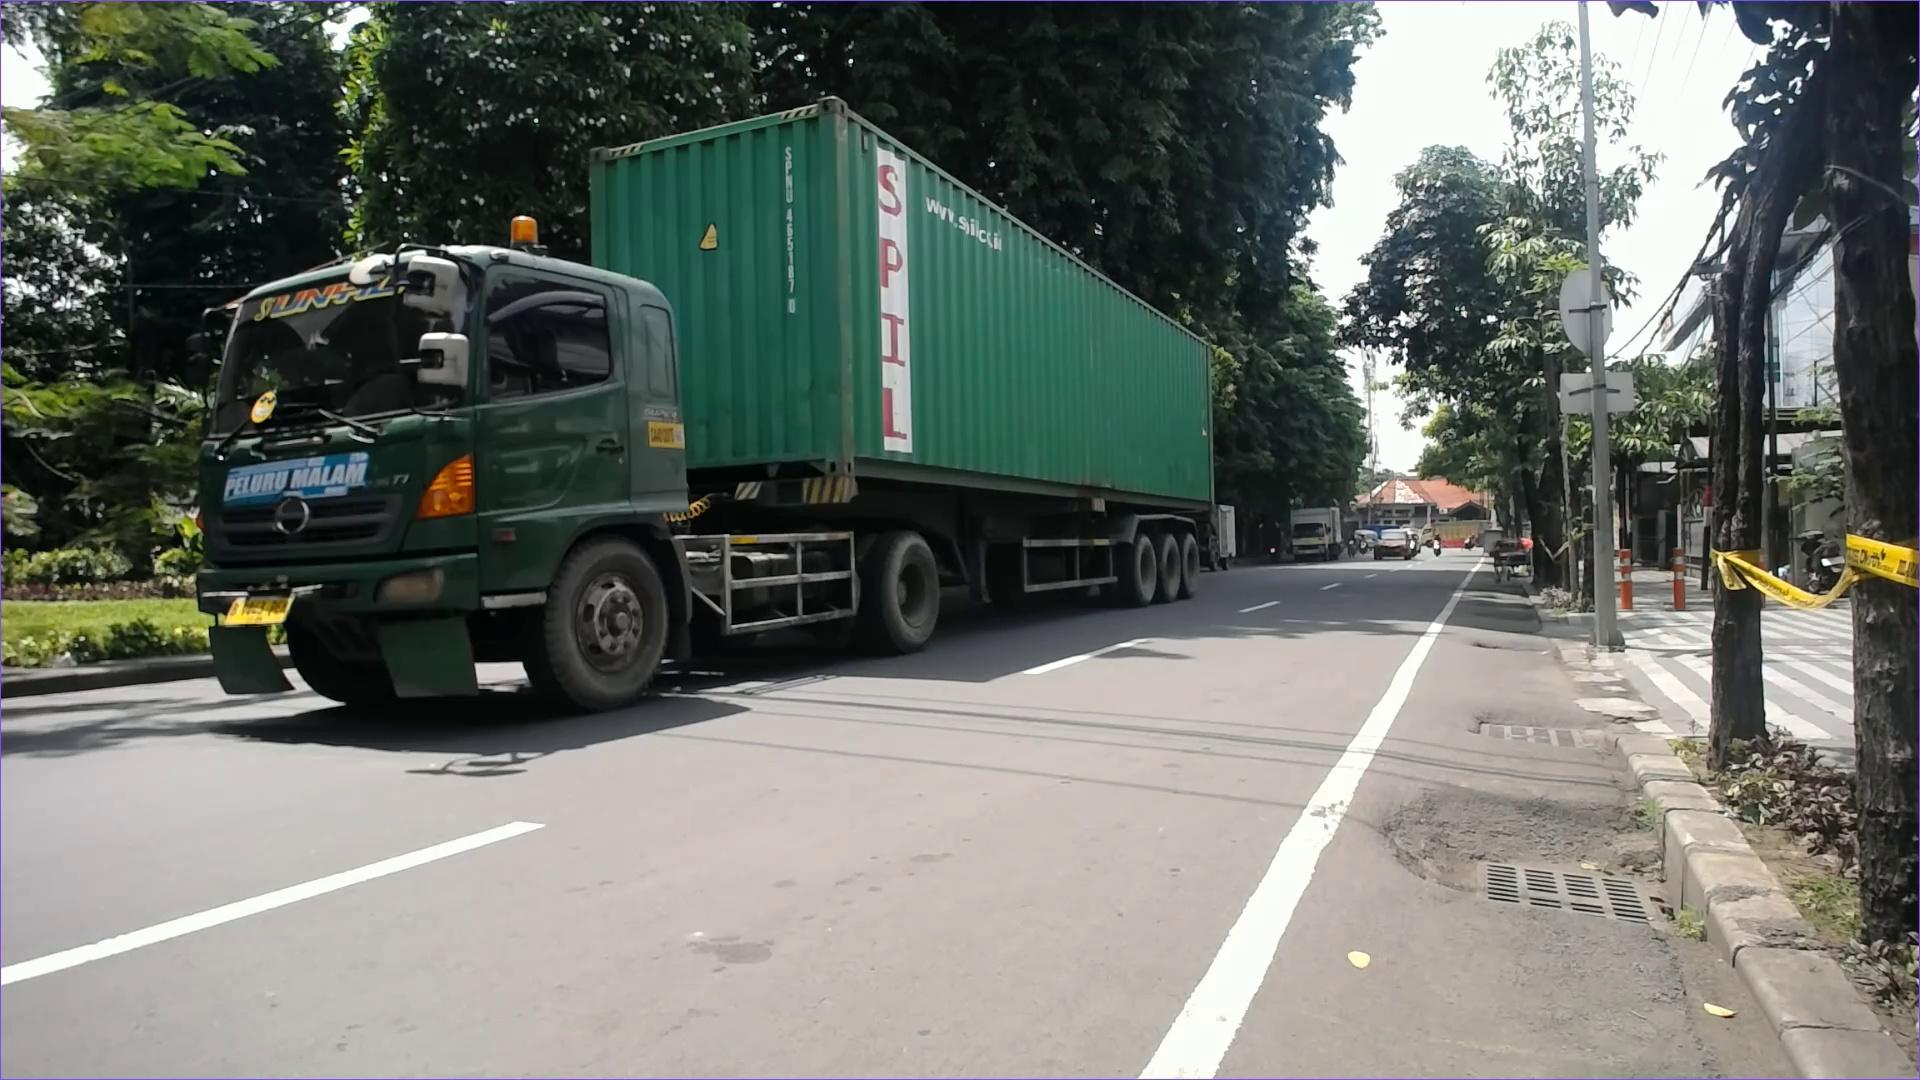
\includegraphics[scale=0.2]{gambar/bab3-citra-asli.jpg}
  \caption{Data citra sebelum dilakukan praproses}
  \label{fig:citraasli}
  
\end{figure}

\begin{figure}[htbp]
  \centering

  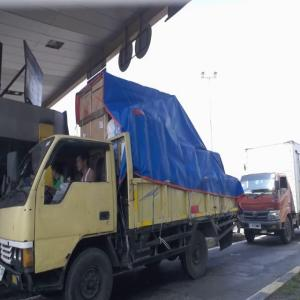
\includegraphics[scale=0.45]{gambar/bab3-citra-300x300.jpg}
  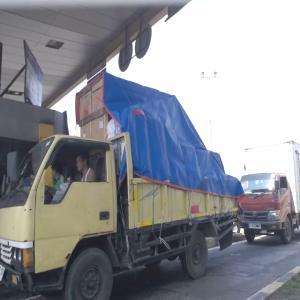
\includegraphics[scale=0.45]{gambar/bab3-citra-300x300-brightness-up.jpg}
  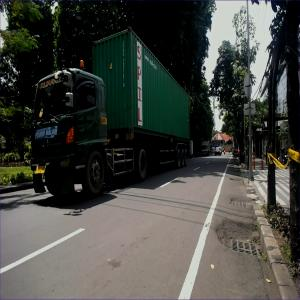
\includegraphics[scale=0.45]{gambar/bab3-citra-300x300-brightness-down.jpg}

  \caption{\centering Data citra setelah dilakukan praproses, (kiri) setelah di-\emph{resize} ke ukuran 300x300, (tengah) citra 300x300 dengan kecerahan dan paparan naik, (kanan) citra 300x300 dengan kecerahan dan paparan turun}
  \label{fig:preprocessingdata}
\end{figure}

\textbf{Pelatihan data} dilakukan setelah data telah dipersiapkan. Data latih yang telah disiapkan akan digunakan untuk melatih model \emph{machine learning} dengan menggunakan \emph{framework} PyTorch. Model yang digunakan adalah SSD-MobileNet-V2 yang telah dilatih sebelumnya (\emph{pre-trained model}) dengan menggunakan dataset COCO. Proses pelatihan ini akan menghasilkan model yang dapat digunakan untuk mendeteksi kendaraan \emph{overdimension}. Gambar \ref{fig:trainingdata} menunjukkan proses pelatihan data yang telah dilakukan.

\subsection{\emph{Hardware}}

Pada bagian ini, dilakukan beberapa tahapan, yaitu:
\begin{enumerate}[nolistsep]
  \item Implementasi hasil pelatihan di \emph{Edge Device} di:
  \begin{enumerate}[nolistsep]
    \item Jetson Nano, dan
    \item Beelink Gemini T34
  \end{enumerate} 
  \item Desain dan pencetakan wadah alat
\end{enumerate}

\textbf{Implementasi hasil pelatihan di \emph{Edge Device}} dilakukan setelah model \emph{machine learning} dilatih. Model yang telah dilatih akan diimplementasikan di \emph{Edge Device} yang telah disiapkan, yaitu Jetson Nano dan Beelink Gemini T34. Implementasi ini bertujuan untuk mendeteksi kendaraan \emph{overdimension} secara \emph{real-time} dan mengintegrasikan hasil deteksi dengan sistem yang ada. Gambar \ref{fig:implementationedgedevice} menunjukkan proses implementasi model \emph{machine learning} di \emph{Edge Device} yang telah dilakukan.

\begin{figure}
  \centering

  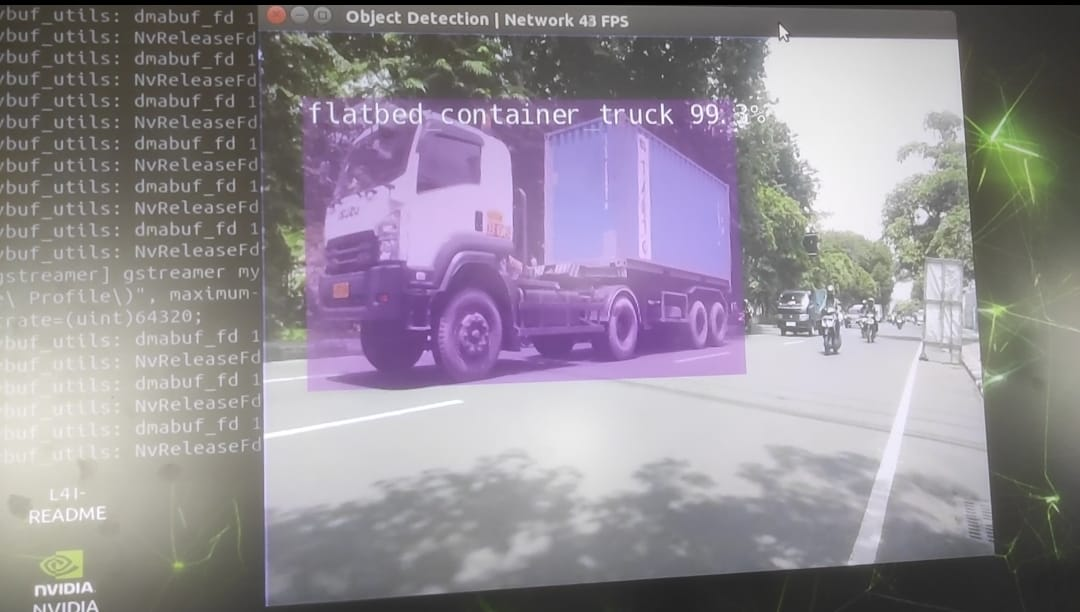
\includegraphics[scale=0.4]{gambar/bab3-implementasi-di-jetson.jpeg}

  \caption{\centering Implementasi Model \emph{Machine Learning} di \emph{Edge Device}, (atas) Jetson Nano, (bawah) Beelink Gemini T34}
  \label{fig:implementationedgedevice}
\end{figure}

\textbf{Desain dan pencetakan wadah alat} dilakukan setelah model \emph{machine learning} berhasil diimplementasikan di \emph{Edge Device}. Wadah alat ini berfungsi sebagai tempat untuk meletakkan \emph{Edge Device} dan kamera yang digunakan untuk mendeteksi kendaraan \emph{overdimension}. Gambar \ref{fig:designcontainercamera}, \ref{fig:designcontainerjetson}, dan \ref{fig:designcontainerbeelink} masing-masing menunjukkan desain wadah kamera, wadah Jetson Nano, dan wadah Beelink Gemini T34 yang telah dibuat.

\begin{figure}
  \centering

  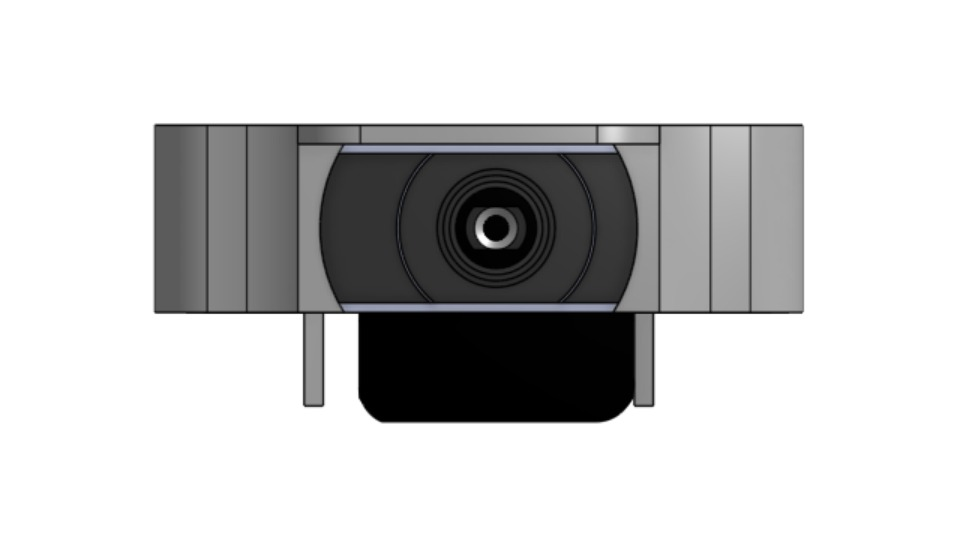
\includegraphics[scale=0.16]{gambar/bab3-tampak-depan-case-camera.jpeg}
  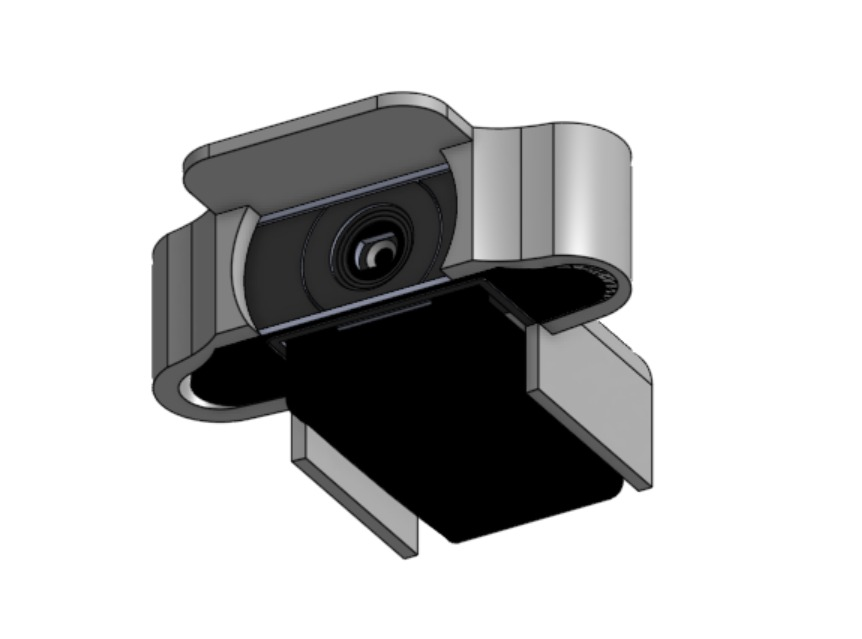
\includegraphics[scale=0.16]{gambar/bab3-tampak-samping-case-camera.jpeg}
  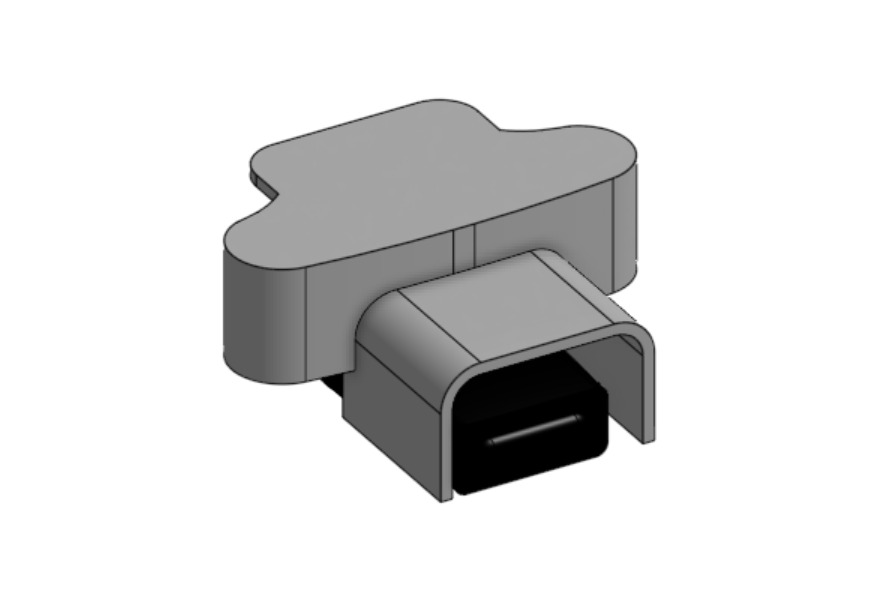
\includegraphics[scale=0.16]{gambar/bab3-tampak-belakang-case-camera.jpeg}

  \caption{\centering Desain Wadah Kamera, (kiri) Tampak Depan, (tengah) Tampak Samping, (kanan) Tampak Belakang}
  \label{fig:designcontainercamera}
\end{figure}

\begin{figure}
  \centering

  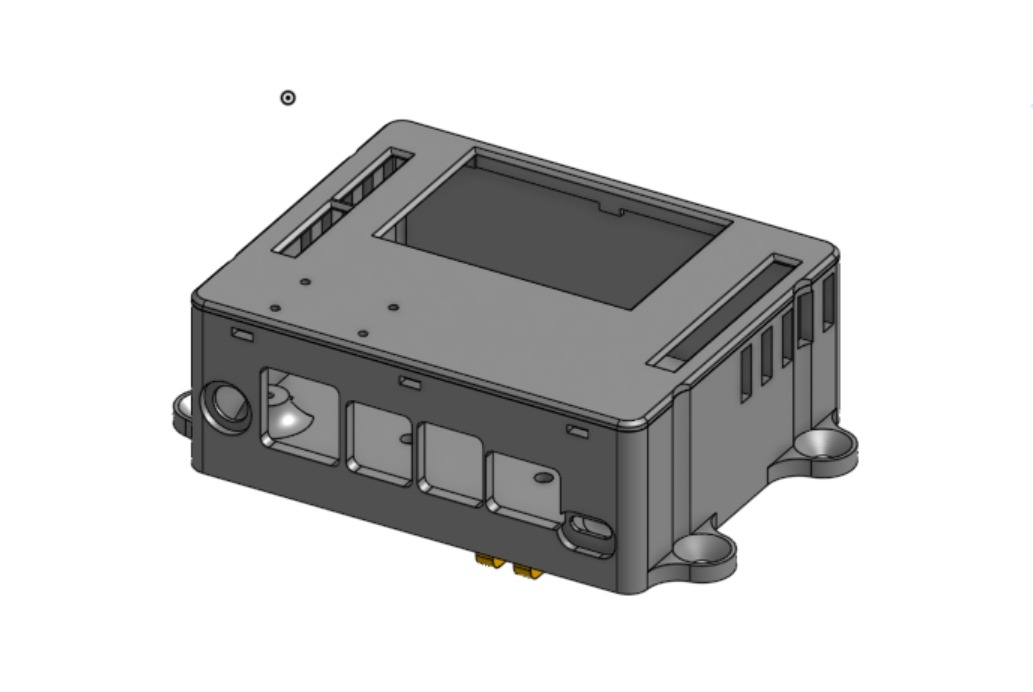
\includegraphics[scale=0.13]{gambar/bab3-tampak-depan-case-jnano.jpeg}
  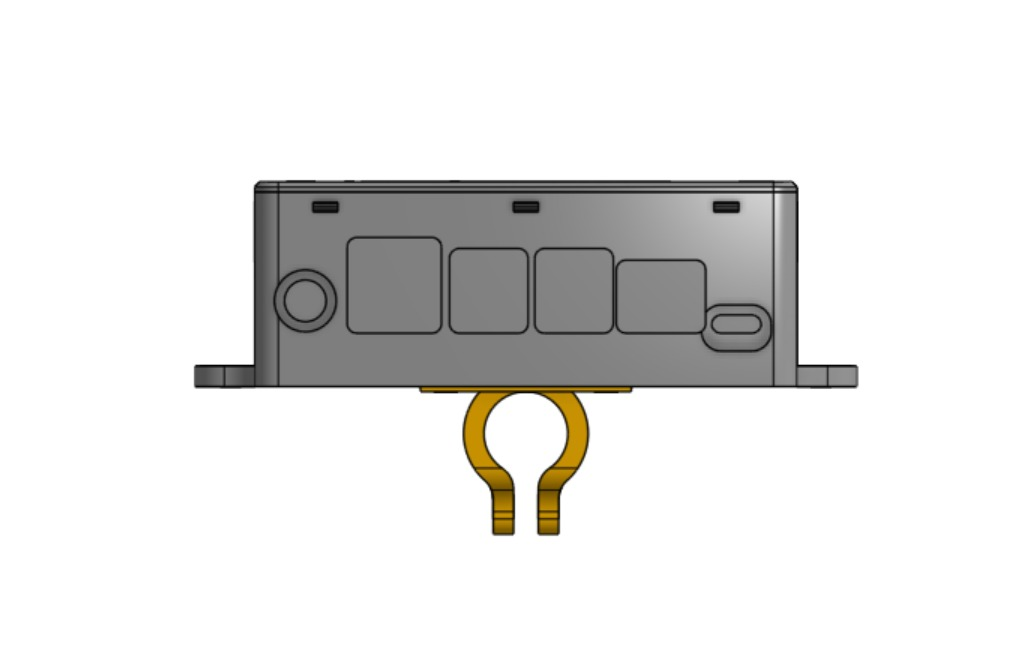
\includegraphics[scale=0.13]{gambar/bab3-tampak-samping-case-jnano.jpeg}
  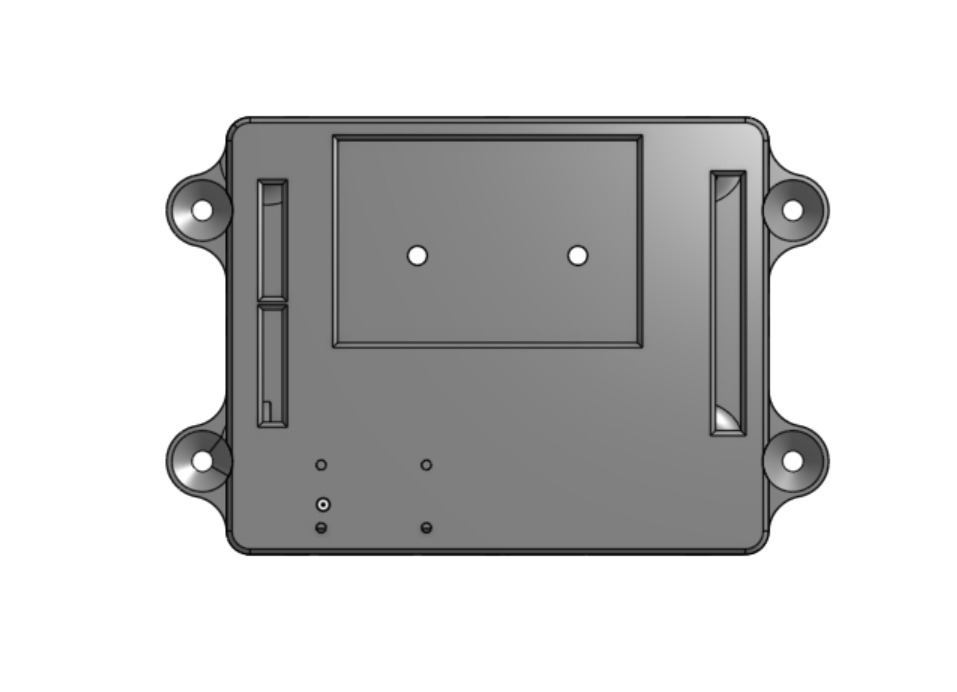
\includegraphics[scale=0.13]{gambar/bab3-tampak-bawah-case-jnano.jpeg}

  \caption{\centering Desain Wadah Jetson Nano, (kiri) Tampak Depan, (tengah) Tampak Samping, (kanan) Tampak Bawah}
  \label{fig:designcontainerjetson}
\end{figure}

Setelah didesain, wadah alat tersebut kemudian dicetak menggunakan printer 3D. Gambar \ref{fig:printcontainer} masing-masing menunjukkan proses pencetakan wadah kamera, wadah Jetson Nano, dan wadah Beelink Gemini T34 yang telah dicetak.

\begin{figure}
  \centering

  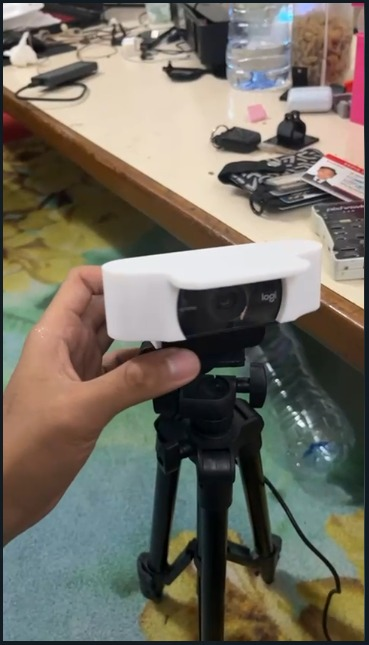
\includegraphics[scale=0.37]{gambar/bab3-case-camera-printed.jpeg}
  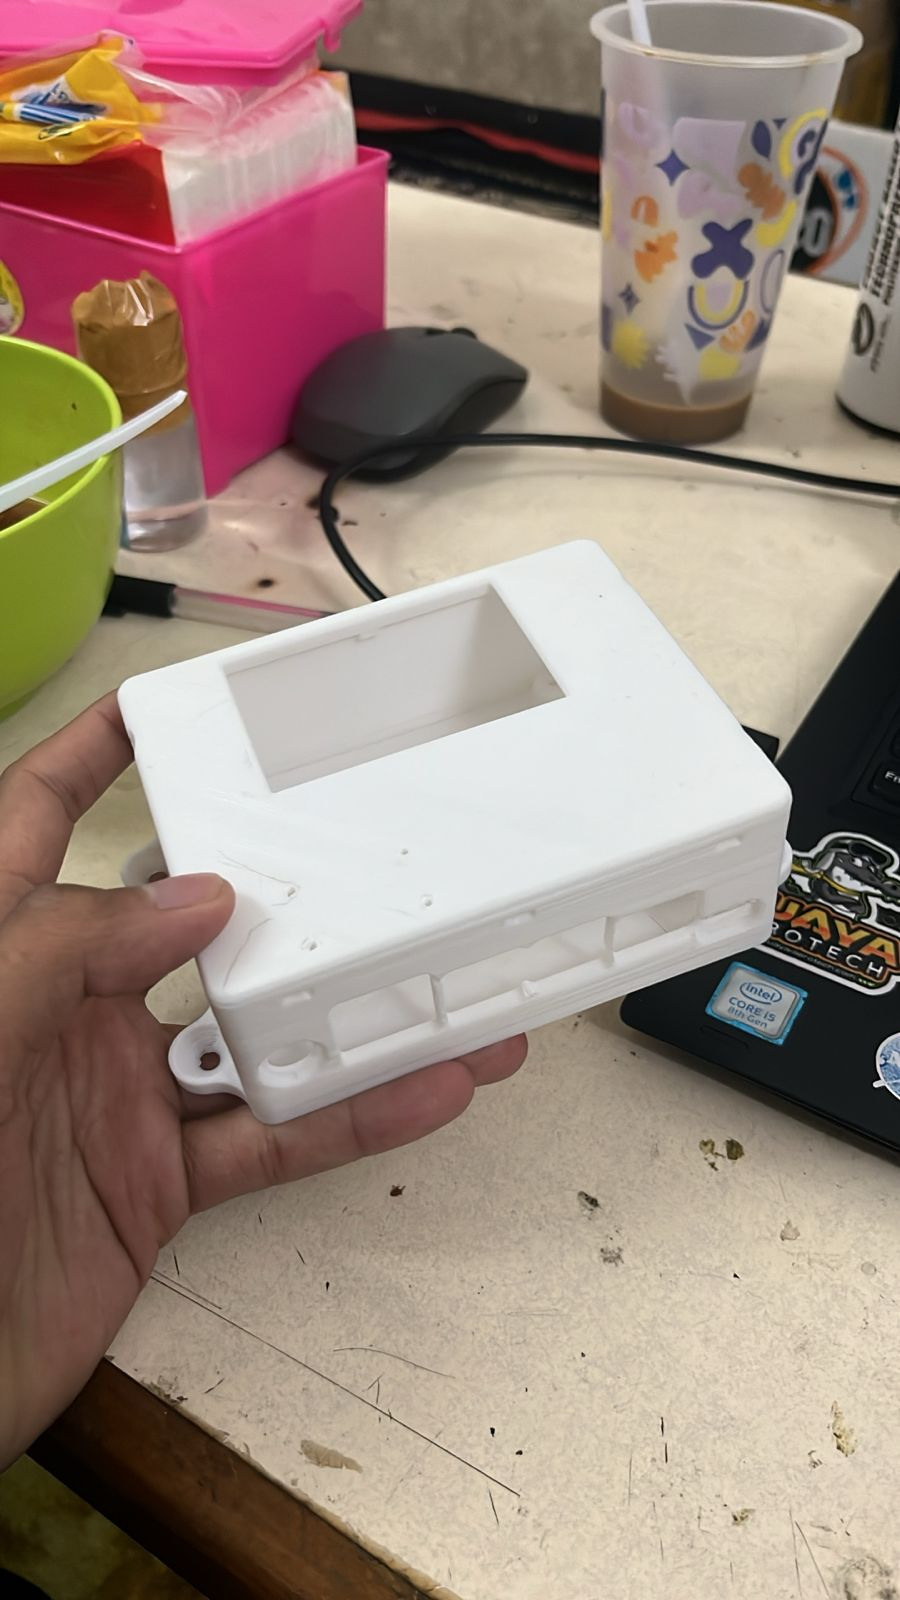
\includegraphics[scale=0.15]{gambar/bab3-case-jnano-printed.jpeg}

  \caption{\centering Hasil Pencetakan Wadah, (kiri) Wadah Kamera, (kanan) Wadah Jetson Nano}
  \label{fig:printcontainer}
\end{figure}

\subsection{\emph{Software - Backend}}

Pada bagian ini, dilakukan beberapa tahapan, yaitu:
\begin{enumerate}[nolistsep]
  \item Membuat daftar fitur aplikasi
  \item Desain basis data
  \item Desain class diagram
  \item Implementasi class diagram
\end{enumerate}

\textbf{Membuat daftar fitur aplikasi} dilakukan untuk menentukan fitur-fitur yang akan ada pada aplikasi, sehingga dapat mempermudah desain basis data dan desain class diagram. Fitur-fitur yang ada pada aplikasi ini adalah:
\begin{itemize}[nolistsep]
  \item Pendaftaran akun
  \item Login
  \item Dashboard berbeda untuk admin dan operator
  \item Analitik data
  \item Notifikasi
  \item Verifikasi pelanggaran
  \item Edit profil
  \item Ubah kata sandi
  \item Lupa kata sandi
\end{itemize}

Sehingga dapat disimpulkan bahwa aplikasi ini memiliki 2 jenis pengguna, yaitu admin dan operator. Admin memiliki akses penuh terhadap aplikasi, sedangkan operator hanya dapat mengakses fitur-fitur tertentu saja, contohnya operator tidak bisa mendapatkan semua user yang terdaftar di aplikasi sedangkan admin bisa.

\textbf{Desain basis data} dilakukan untuk menentukan struktur basis data yang akan digunakan pada aplikasi. Basis data yang digunakan adalah basis data \emph{relational} dengan menggunakan \emph{PostgreSQL}. Tabel-tabel yang ada pada basis data ini adalah:
\begin{itemize}[nolistsep]
  \item Tabel \emph{Users}
  \item Tabel \emph{TollGates}
  \item Tabel \emph{Notifications}
  \item Tabel \emph{VehicleDetections}
  \item Tabel \emph{Images}
\end{itemize}

Gambar \ref{fig:databasedesign} menunjukkan desain basis data yang telah dibuat menggunakan website \emph{dbdiagram.io}. Desain basis data ini menggambarkan relasi antar tabel yang ada pada basis data. Tabel-tabel tersebut memiliki relasi satu sama lain, sehingga dapat saling berhubungan dan mempermudah dalam pengolahan data.
\begin{figure}[htbp]
  \centering

  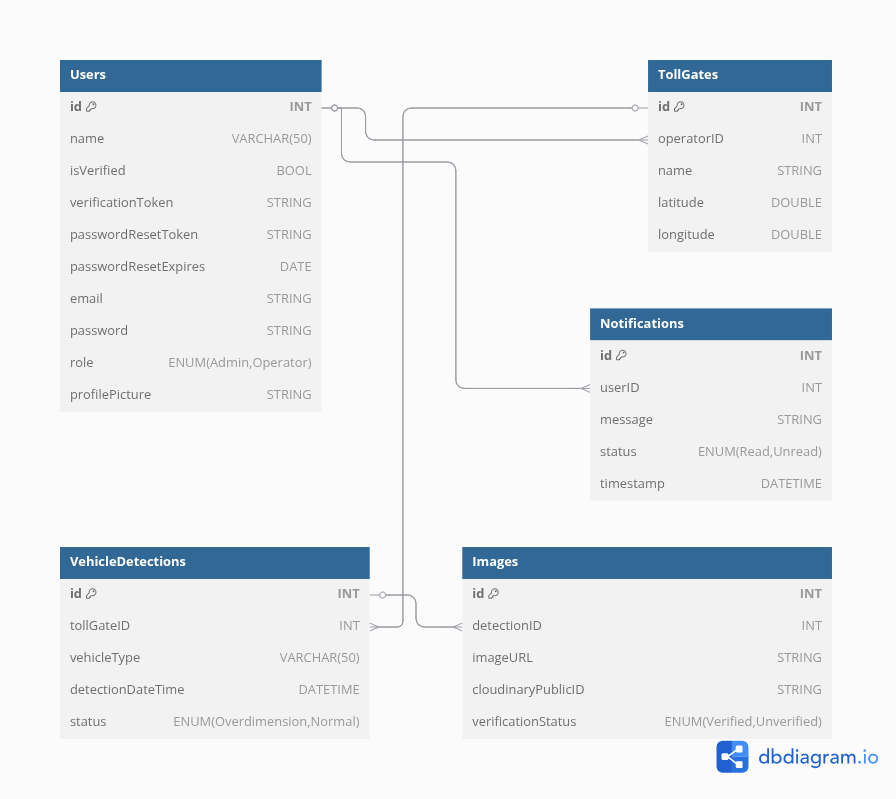
\includegraphics[scale=0.35]{gambar/bab3-desain-database.png}

  \caption{Desain Basis Data}
  \label{fig:databasedesign}
\end{figure}
Dari tabel-tabel yang ada pada basis data tersebut, dapat dilihat bahwa:

\begin{itemize}[nolistsep]
  \item Tabel \emph{Users} berisi data pengguna aplikasi, baik admin maupun operator. Tabel ini memiliki relasi \emph{one to many} dengan tabel \emph{VehicleDetections} dan \emph{Notifications}
  \item Tabel \emph{TollGates} berisi data gerbang tol yang ada. Tabel ini memiliki relasi \emph{one to many} dengan tabel \emph{VehicleDetections}
  \item Tabel \emph{Notifications} berisi data notifikasi yang ada pada aplikasi. Baik notifikasi yang dikirimkan oleh sistem maupun notifikasi yang dikirimkan oleh admin kepada operator.
  \item Tabel \emph{VehicleDetections} berisi data deteksi kendaraan yang ada pada aplikasi. Di tabel inilah dilakukan verifikasi status dari kendaraan, apakah kendaraan tersebut \emph{overdimension} atau tidak. Tabel ini memiliki relasi \emph{one to many} dengan tabel \emph{Images}
  \item Tabel \emph{Images} berisi data gambar kendaraan \emph{overdimension} yang terdeteksi. Gambar tidak disimpan dalam basis data, tetapi hanya menyimpan \emph{link} gambar yang ada pada \emph{cloud storage} Cloudinary.
\end{itemize}

\subsection{\emph{Cloud}}

\lipsum[1]

\subsection{\emph{Software} - Aplikasi \emph{Mobile}}

\lipsum[1]
\cleardoublepage

% Bab 4 pengujian dan analisis
\chapter{PENGUJIAN DAN ANALISIS}
\label{chap:pengujiananalisis}

\section{Alat dan Bahan}
\label{sec:alatdanbahan}

\subsection{Perangkat Pelatihan Model \emph{Machine Learning}}

Pelatihan model dilakukan pada perangkat komputer dengan spesifikasi sebagai berikut:

\begin{table}[htbp]
  \centering
  \begin{tabular}{|l|l|}
  \hline
  \textbf{Prosesor} & Intel® Core™ i5-1235U \\
  \hline
  \textbf{GPU} & NVIDIA Geforce MX550 GDDR6 (2GB VRAM) \\
  \hline
  \textbf{RAM} & 16GB DDR4 \\
  \hline
  \textbf{Penyimpanan} & 512GB SSD M.2 PCIe \\
  \hline
  \textbf{Sistem Operasi} & Linux Ubuntu 22.04 Jammy Jellyfish \\
  \hline
  \textbf{Framework} & Tensorflow 2.15 \& PyTorch 2.3.0 \\
  \hline
  \textbf{Lingkungan Pengembangan} & Python 3.10.12 \\
  \hline
  \end{tabular}
  \caption{Spesifikasi perangkat \emph{laptop} untuk pelatihan model}
  \label{tab:training_laptop_specs}
\end{table}
Model yang digunakan adalah SSD MobileNetV2 yang dilatih menggunakan dataset kendaraan hasil anotasi sendiri dan milik dari penelitian Prismadika Yuniar \parencite*{prismadika2023}. Proses pelatihan dilakukan selama 30 dan 50 \emph{epoch} dengan batch size 16, learning rate 0.01, dan \emph{scheduler} antara CosineAnnealingLR dan MultiStepLR. Dataset terdiri dari masing-masing 165 dan 200 gambar kendaraan sebelum augmentasi, yang dibagi menjadi data latih (80\%) dan data validasi (20\%).

\subsection{\emph{Edge Device} untuk \emph{Inference}}

Untuk menjalankan sistem deteksi secara real-time, model hasil pelatihan dikonversi dari format PyTorch Tensor (.pt) ke ONNX (.onnx) dengan tujuan untuk diimplementasikan pada perangkat edge. Pengujian dilakukan pada perangkat \emph{edge} yang memiliki spesifikasi sebagai berikut:

\subsubsection{Perangkat 1: NVIDIA Jetson Nano 4GB}

Perangkat pertama yang digunakan adalah NVIDIA Jetson Nano 4GB yang merupakan sistem berbasis ARM yang dirancang untuk aplikasi edge computing dengan kemampuan grafis yang optimal. Jetson Nano memiliki GPU Maxwell dengan 128 CUDA cores yang memungkinkan pemrosesan model deep learning secara efisien. Kamera yang digunakan pada pengujian ini adalah Logitech C920 HD Pro USB Webcam yang dapat memberikan kualitas video 1080p pada 30 FPS, cukup untuk pengolahan deteksi kendaraan secara real-time. Tabel \ref{tab:jetson_nano_specs} menunjukkan spesifikasi perangkat Jetson Nano yang digunakan dalam penelitian ini.

\begin{table}[htbp]
  \centering
  \begin{tabular}{|l|l|}
  \hline
  \textbf{Perangkat} & NVIDIA Jetson Nano 4GB \\
  \hline
  \textbf{CPU} & Quad-core ARM Cortex-A57 MPCore processor \\
  \hline
  \textbf{GPU} & NVIDIA Maxwell 128 NVIDIA CUDA® cores \\
  \hline
  \textbf{RAM} & 4 GB 64-bit LPDDR4, 1600MHz 25.6 GB/s \\
  \hline
  \textbf{Penyimpanan} & 16 GB eMMC 5.1 \\
  \hline
  \textbf{Sistem Operasi} & Linux Ubuntu 18.04 Bionic Beaver \\
  \hline
  \textbf{Kamera} & Logitech C920 HD Pro USB Webcam \\
  \hline
  \textbf{Lingkungan Pengembangan} & Python 3.6.9 \\
  \hline
  \end{tabular}
  \caption{Spesifikasi perangkat \emph{edge} pertama untuk \emph{inference}}
  \label{tab:jetson_nano_specs}
\end{table}

\subsubsection{Perangkat 2: Beelink Gemini T34}

Selain menggunakan Jetson Nano, perangkat kedua yang digunakan dalam pengujian adalah Beelink Gemini T34, sebuah mini PC dengan kemampuan komputasi yang cukup untuk aplikasi deteksi real-time. Beelink Gemini T34 dilengkapi dengan prosesor Intel Celeron dan GPU Intel HD Graphics 600, yang mendukung akselerasi inferensi untuk model deep learning. Perangkat ini cocok untuk pengolahan data video dan real-time inferencing, sehingga memudahkan implementasi model pada sistem gerbang tol. Tabel \ref{tab:beelink_t34_specs} menunjukkan spesifikasi perangkat Beelink Gemini T34 yang digunakan dalam penelitian ini.

\begin{table}[htbp]
  \centering
  \begin{tabular}{|l|l|}
  \hline
  \textbf{Perangkat} & Beelink Gemini T34 \\
  \hline
  \textbf{CPU} & Intel Celeron N3450 Quad-core \\
  \hline
  \textbf{GPU} & Intel HD Graphics 500 \\
  \hline
  \textbf{RAM} & 8 GB DDR3L \\
  \hline
  \textbf{Penyimpanan} & 256 GB SSD M.2 SATA \\
  \hline
  \textbf{Sistem Operasi} & Linux Ubuntu 20.04 Focal Fossa \\
  \hline
  \textbf{Kamera} & Logitech C920 HD Pro USB Webcam \\
  \hline
  \textbf{Lingkungan Pengembangan} & Python 3.8.10 \\
  \hline
  \end{tabular}
  \caption{Spesifikasi perangkat \emph{edge} kedua untuk \emph{inference}}
  \label{tab:beelink_t34_specs}
\end{table}

Dengan penggunaan dua perangkat ini, yaitu NVIDIA Jetson Nano yang lebih fokus pada aplikasi edge dengan akselerasi GPU untuk deep learning, serta Beelink Gemini T34 yang menawarkan solusi berbasis prosesor Intel untuk komputasi ringan, pengujian dilakukan untuk melihat perbandingan performa dan kecocokan setiap perangkat untuk aplikasi deteksi kendaraan overdimensi secara real-time.

\subsection{Spesifikasi \emph{Server Cloud}}

Untuk mendukung pengolahan backend dan pengelolaan data dari perangkat edge, sistem ini menggunakan \emph{Virtual Private Server} (VPS) yang dihosting di cloud. VPS ini digunakan untuk menjalankan layanan backend seperti manajemen database, penyimpanan data kendaraan yang terdeteksi, serta komunikasi antara perangkat edge dan server cloud. Berikut adalah spesifikasi VPS yang digunakan:

\begin{table}[htbp]
  \centering
  \begin{tabular}{|l|l|}
  \hline
  \textbf{Provider} & Biznet Gio \\
  \hline
  \textbf{Tipe VPS} & Neo Lite \\
  \hline
  \textbf{CPU} & 1 vCPU (Intel Xeon) \\
  \hline
  \textbf{RAM} & 2 GB \\
  \hline
  \textbf{Penyimpanan} & 60 GB SSD \\
  \hline
  \textbf{Sistem Operasi} & Ubuntu 22.04 LTS \\
  \hline
  \textbf{IP Address} & Static Public IP \\
  \hline
  \textbf{Lingkungan Pengembangan} & Node.js v20.19.1  \\
  \hline
  \end{tabular}
  \caption{Spesifikasi Server Cloud untuk Hosting Backend}
  \label{tab:cloud_server_specs}
  \end{table}

\subsection{Lingkungan Pengujian}

Lingkungan pengujian alat dilakukan di Gerbang Tol Dupak 2, Genting Kalianak, Asem Rowo, Surabaya, Jawa Timur. Pengujian dilakukan pada hari Senin, 28 April 2025, Kamis 1 Mei 2025, dan Jumat 2 Mei 2025. Masing-masing hari pengujian dilakukan pada pukul 08:00 - 12:00 WIB. 

Perangkat kamera ditempatkan pada ketinggian ... meter dari permukaan jalan dengan sudut kemiringan 45 derajat ke arah lajur kendaraan. Posisi ini dipilih untuk memastikan penangkapan gambar yang optimal dari bagian depan kendaraan yang melintasi gerbang tol. Jarak pengambilan gambar dari perangkat kamera ke objek kendaraan ... meter.

Lalu lintas kendaraan selama pengujian tercatat rata-rata 120-150 kendaraan per jam dengan variasi jenis kendaraan meliputi mobil penumpang (55\%), truk ringan (25\%), truk sedang (15\%), dan kendaraan berat (5\%). Perangkat edge ditempatkan di pinggir gerbang tol dengan koneksi internet berkecepatan 3-5 Mbps menggunakan hostpot dari handphone untuk transmisi data ke server cloud. Gambar \ref{fig:testing_environment} menunjukkan setup perangkat pada lokasi pengujian.

% Tambahkan gambar setup pengujian
\begin{figure}[htbp]
  \centering
  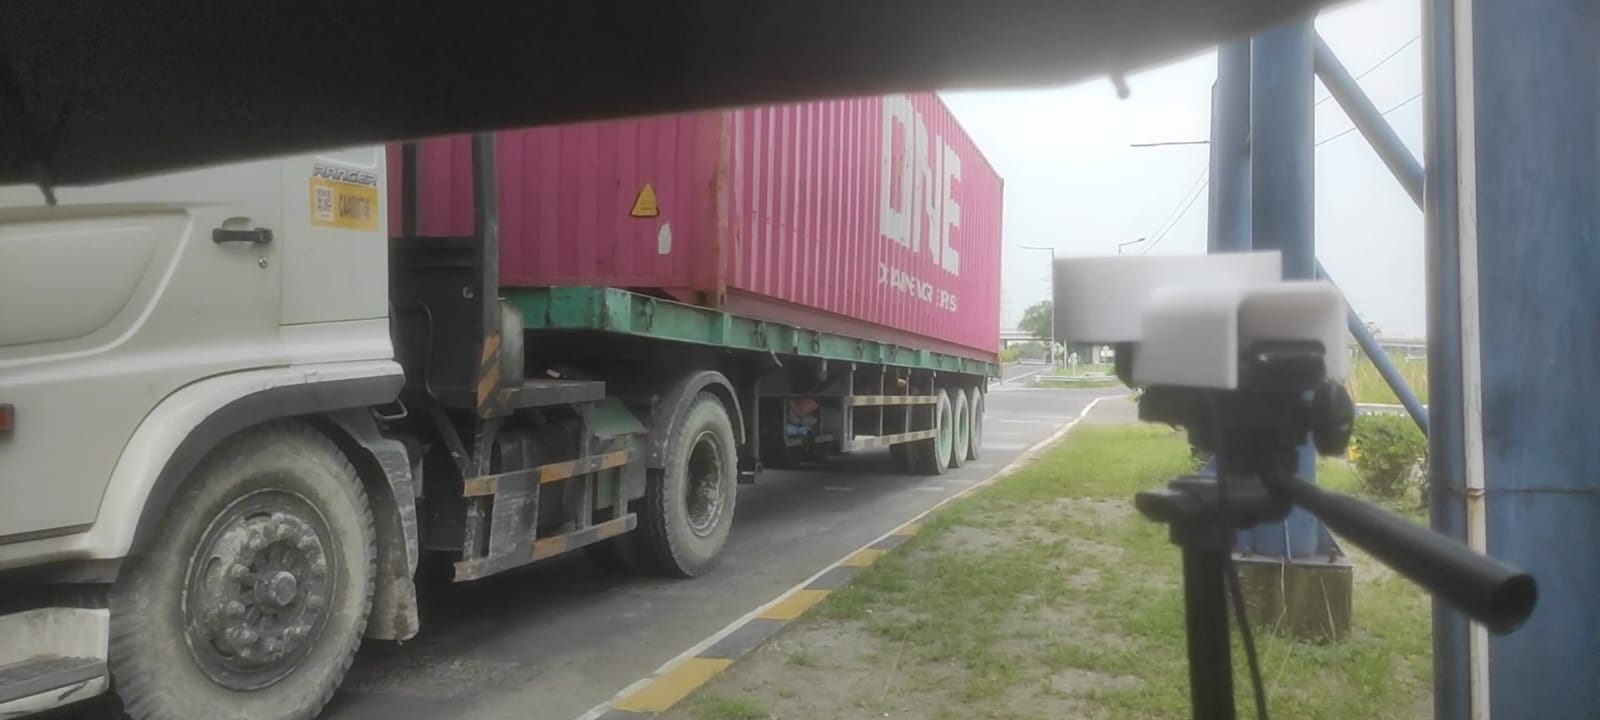
\includegraphics[width=0.8\textwidth]{gambar/bab4-test-dupak-kamera.jpeg}
  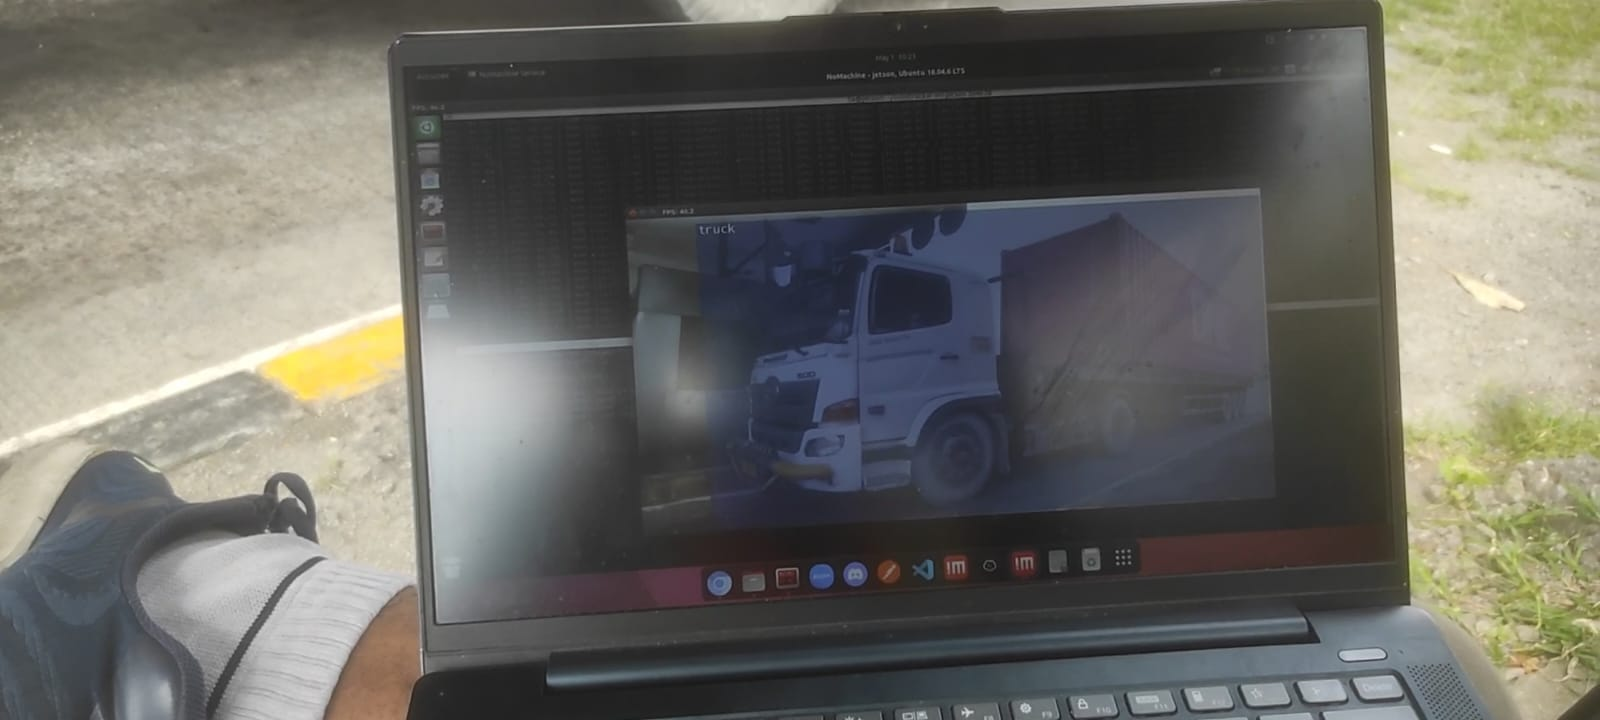
\includegraphics[width=0.8\textwidth]{gambar/bab4-test-dupak-monitor.jpeg}
  \caption{Setup perangkat pada lokasi pengujian di Gerbang Tol Dupak 2}
  \label{fig:testing_environment}
\end{figure}

\section{Model SSD-MobileNetV2}
\label{sec:model_ssd_mobilenetv2}

\subsection{Analisis Hasil Latih Model}

Hasil pelatihan model SSD-MobileNetV2 pada dataset kendaraan dianalisis berdasarkan beberapa metrik evaluasi yang umum digunakan dalam deteksi objek. Model dilatih dengan konfigurasi 16 batch size, learning rate 0.01, dan 4 konfigurasi berbeda, yaitu:

\begin{itemize}[nolistsep]
  \item 30 \emph{epoch} dan \emph{scheduler} CosineAnnealingLR
  \item 30 \emph{epoch} dan \emph{scheduler} MultiStepLR
  \item 50 \emph{epoch} dan \emph{scheduler} CosineAnnealingLR
  \item 50 \emph{epoch} dan \emph{scheduler} MultiStepLR
\end{itemize}\

Selama proses pelatihan, berbagai metrik dipantau untuk menganalisis konvergensi model, meliputi \emph{accuracy}, \emph{precision}, \emph{recall}, \emph{F1 score}, \emph{regression loss}, \emph{classification loss}, dan \emph{total loss}. Grafik di bawah ini menunjukkan hasil pelatihan untuk masing-masing konfigurasi.

\begin{figure}[htbp]
  \centering
  \begin{subfigure}{0.45\textwidth}
    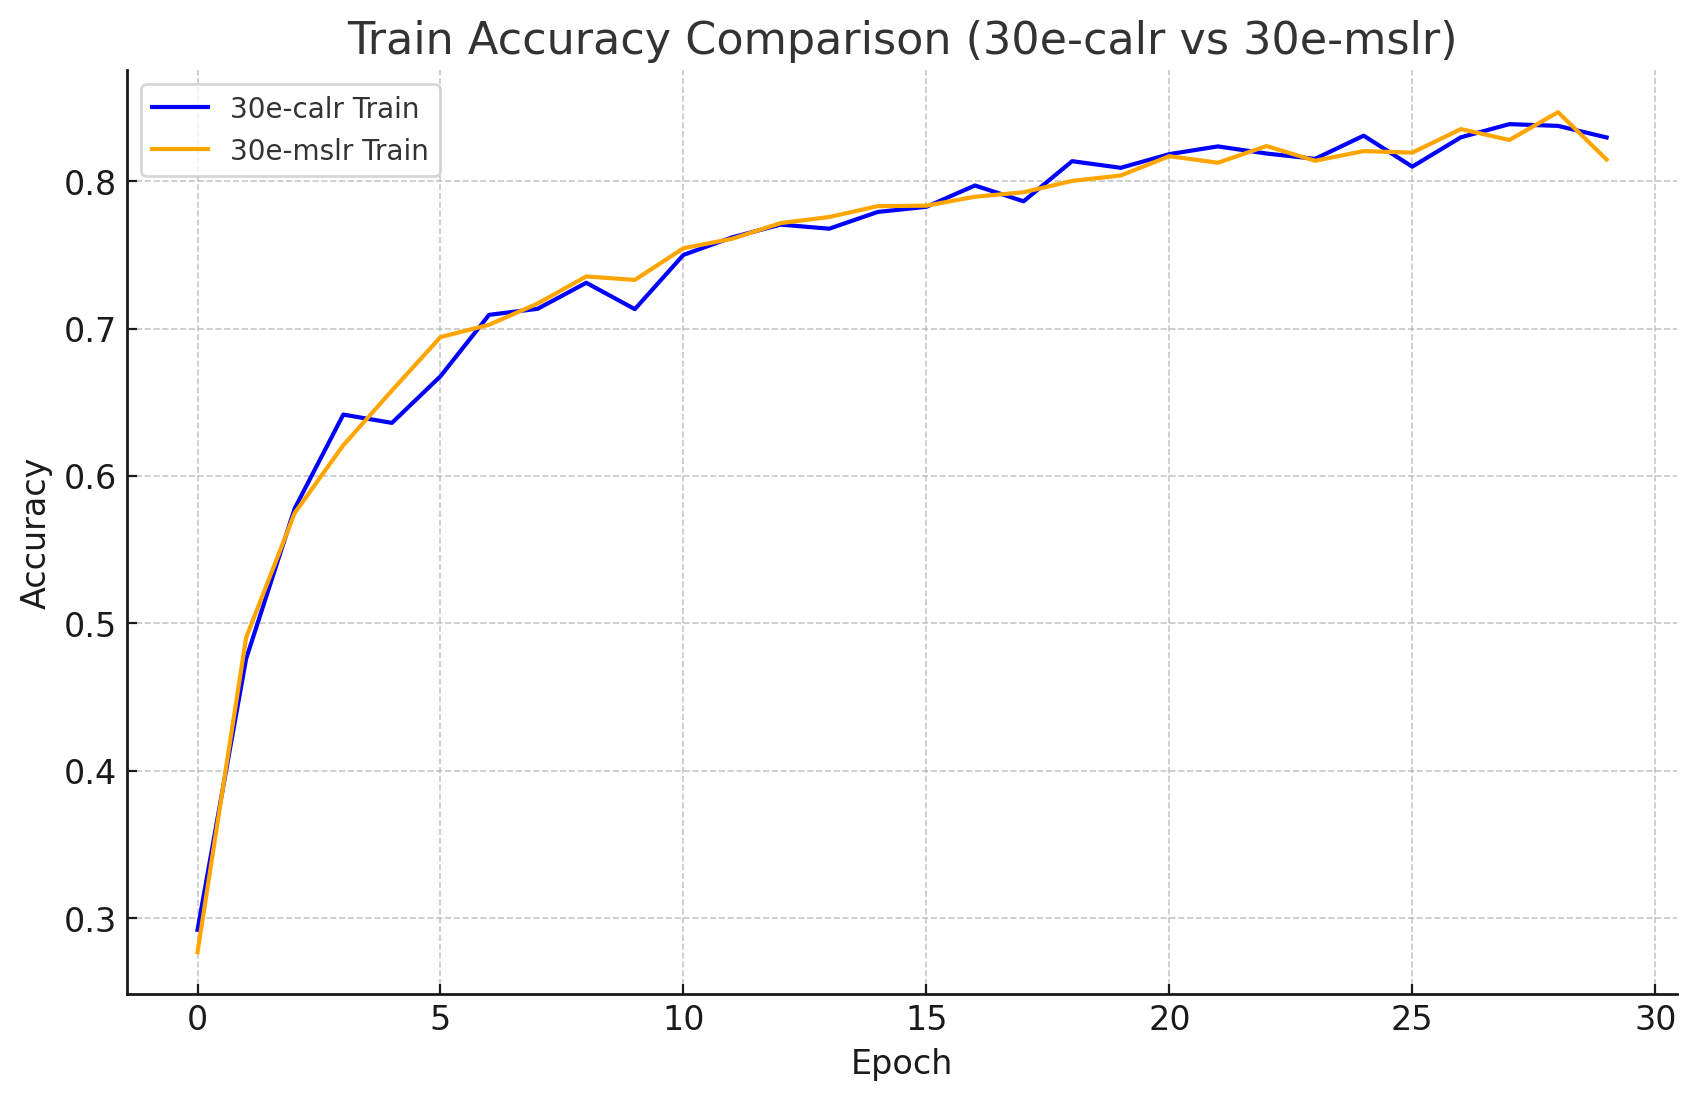
\includegraphics[width=\textwidth]{gambar/bab4-train-acc-30e.png}
    \caption{Accuracy (training) - 30 \emph{epoch}}
  \end{subfigure}
  \hfill
  \begin{subfigure}{0.45\textwidth}
    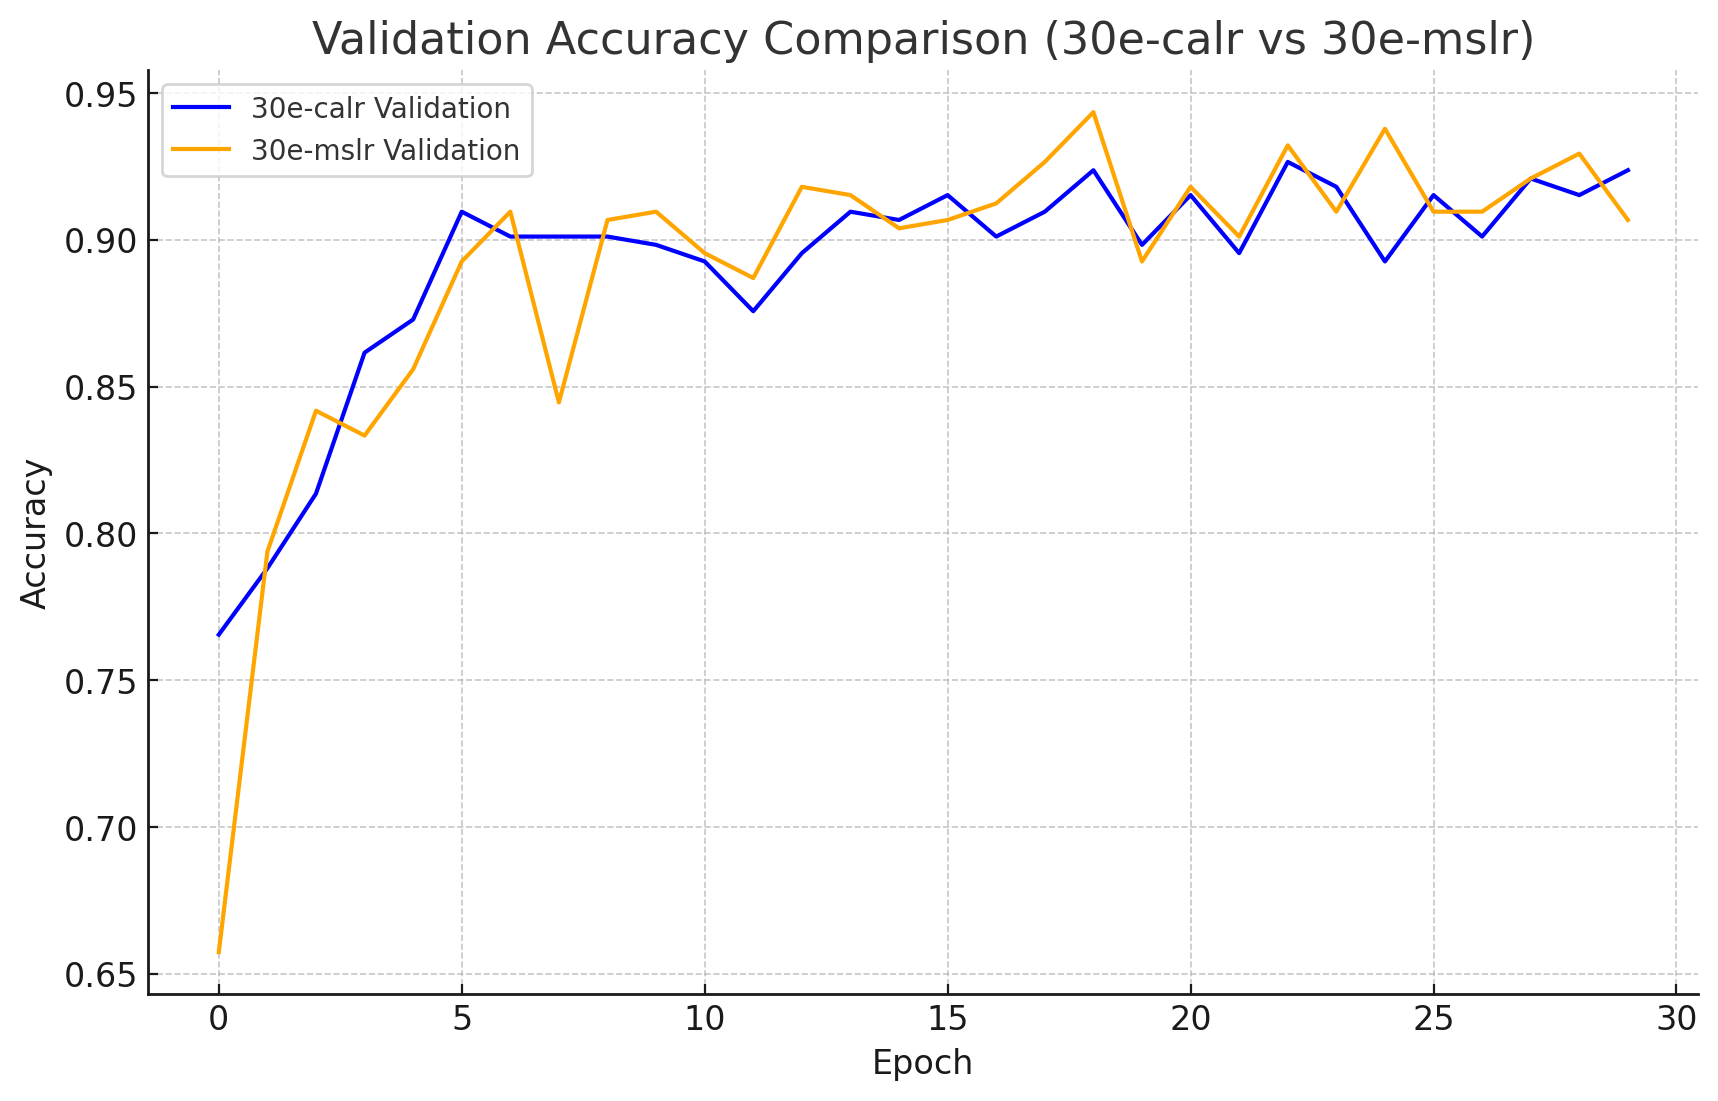
\includegraphics[width=\textwidth]{gambar/bab4-val-acc-30e.png}
    \caption{Accuracy (validation) - 30 \emph{epoch}}
  \end{subfigure}
  \begin{subfigure}{0.45\textwidth}
    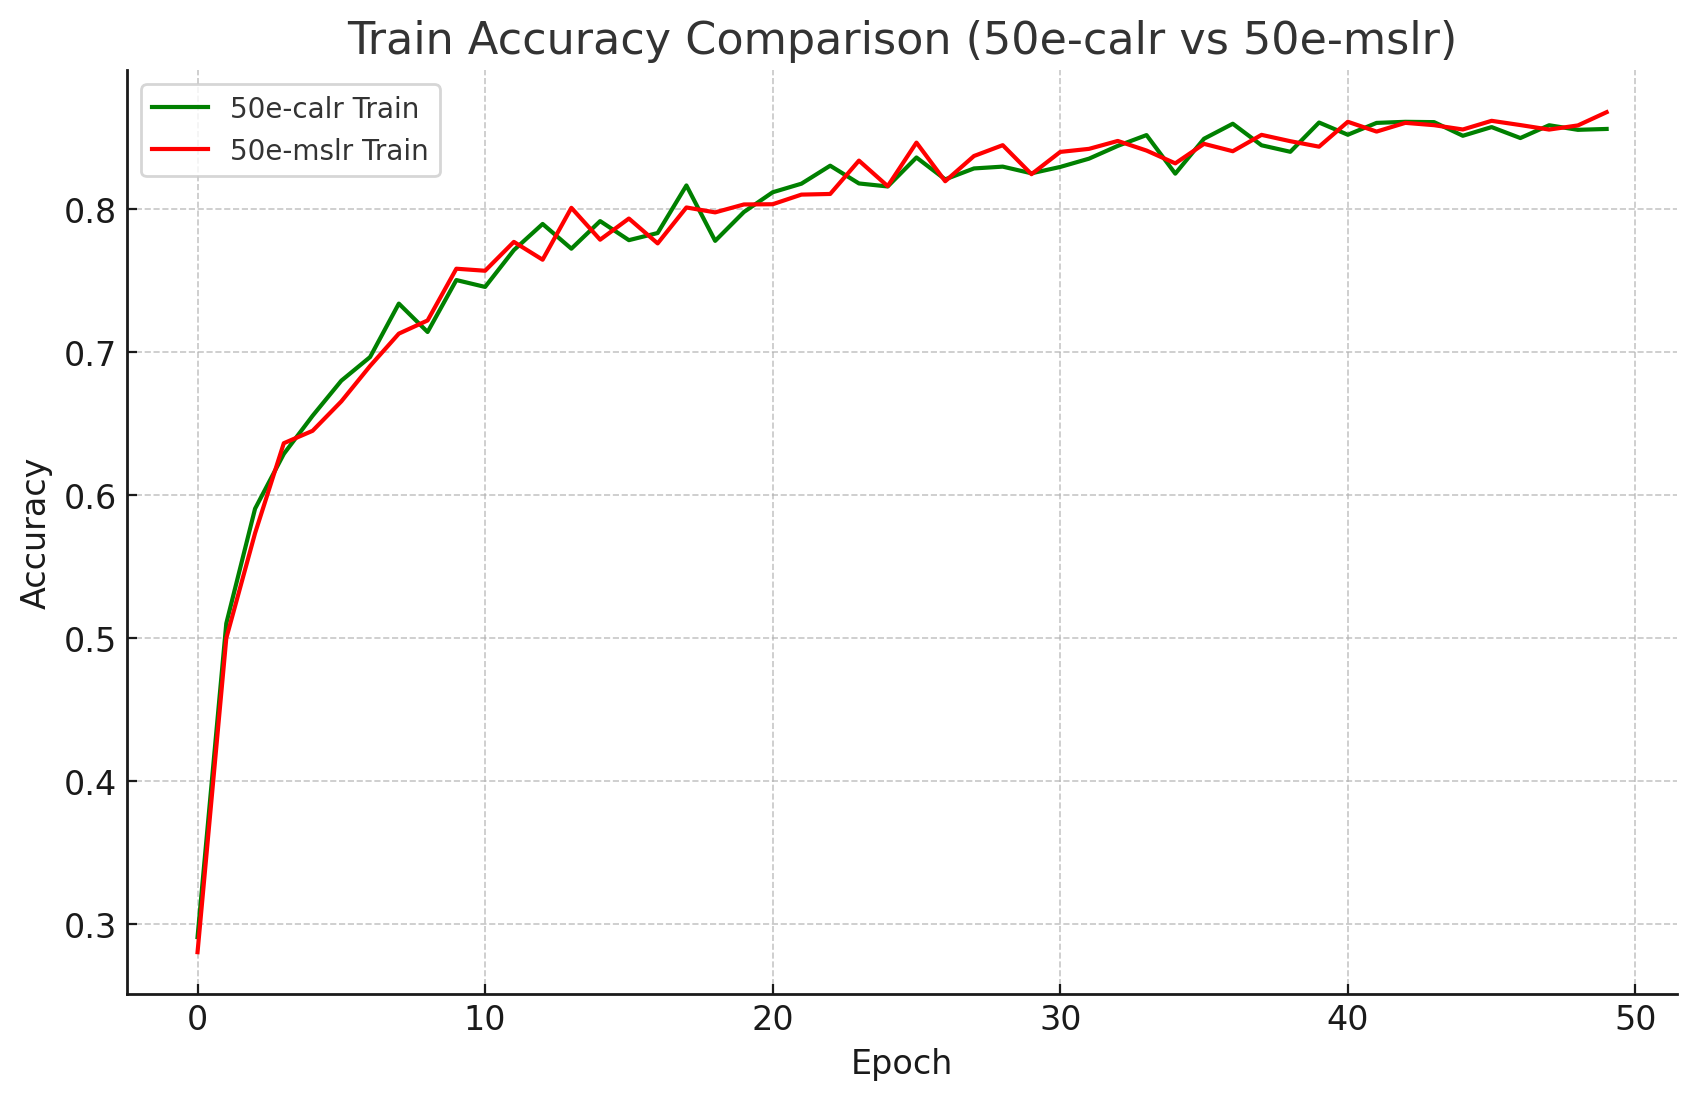
\includegraphics[width=\textwidth]{gambar/bab4-train-acc-50e.png}
    \caption{Accuracy (training) - 50 \emph{epoch}}
  \end{subfigure}
  \hfill
  \begin{subfigure}{0.45\textwidth}
    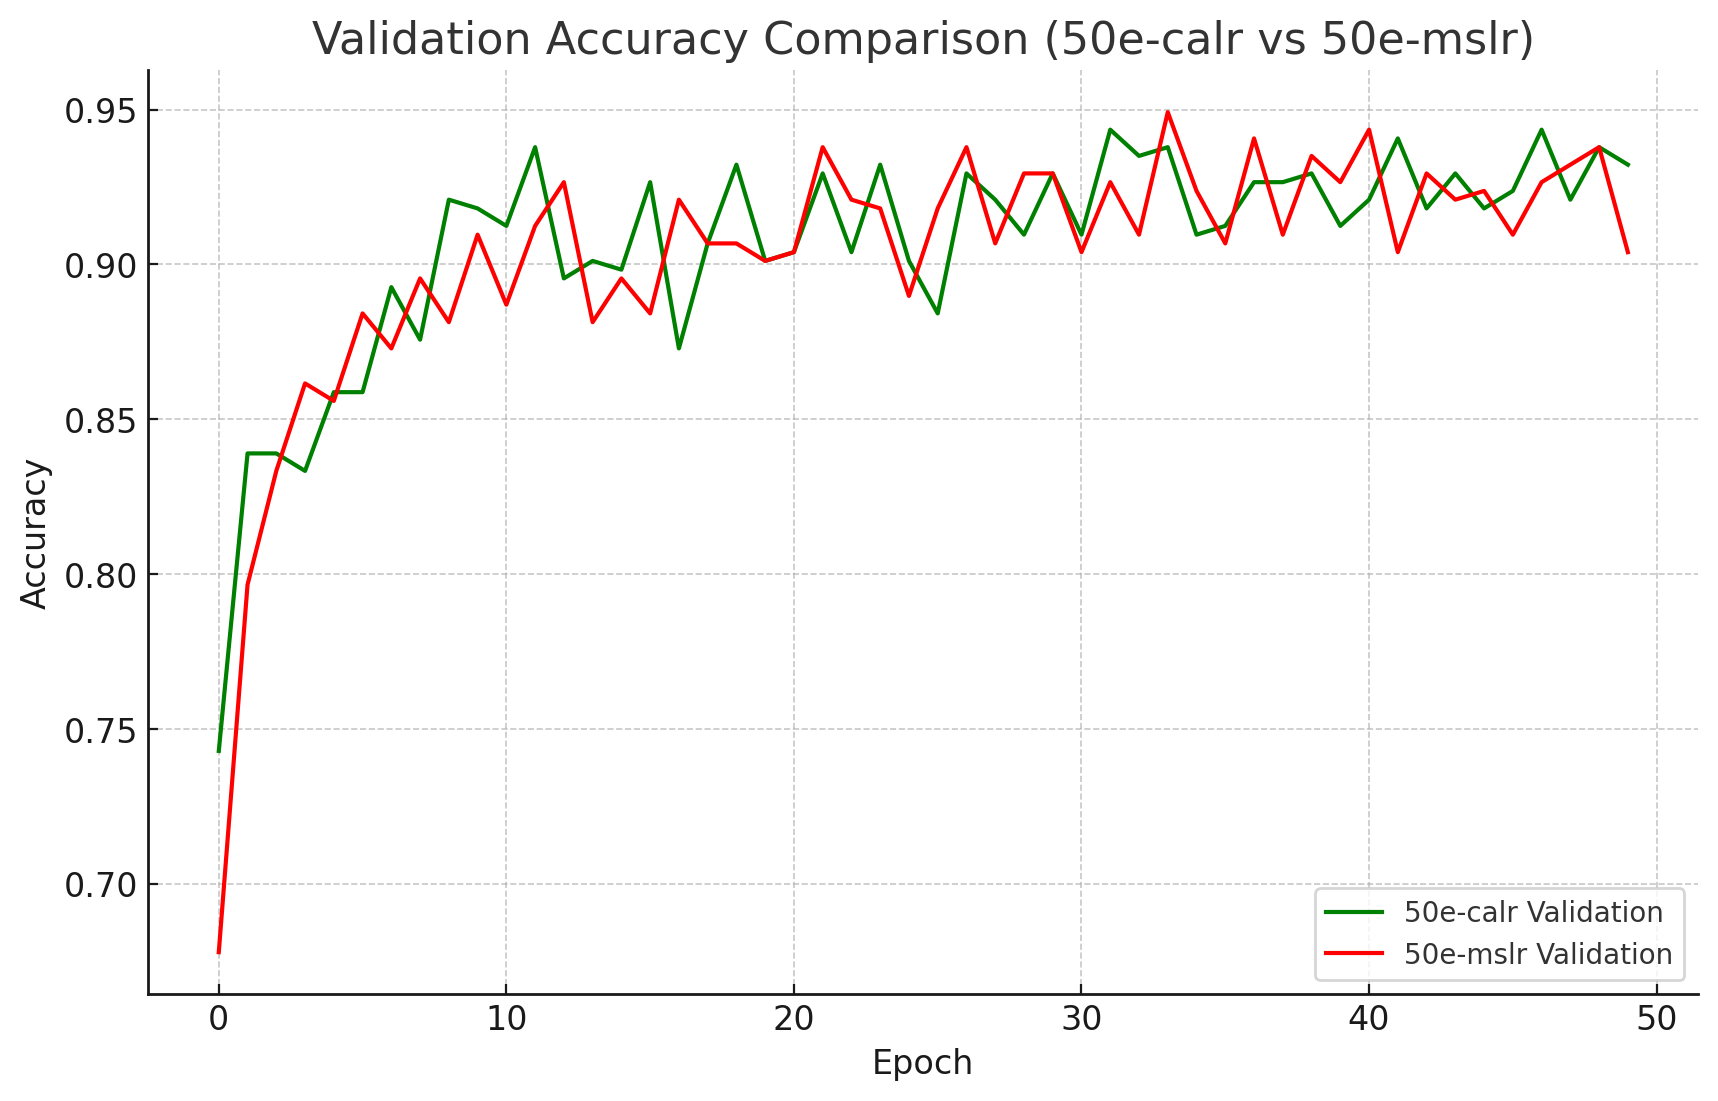
\includegraphics[width=\textwidth]{gambar/bab4-val-acc-50e.png}
    \caption{Accuracy (validation) - 50 \emph{epoch}}
  \end{subfigure}
  \caption{Kurva Accuracy selama proses pelatihan model SSD-MobileNetV2}
  \label{fig:accuracy_curves}
\end{figure}

\begin{figure}[htbp]
  \centering
  \begin{subfigure}{0.45\textwidth}
    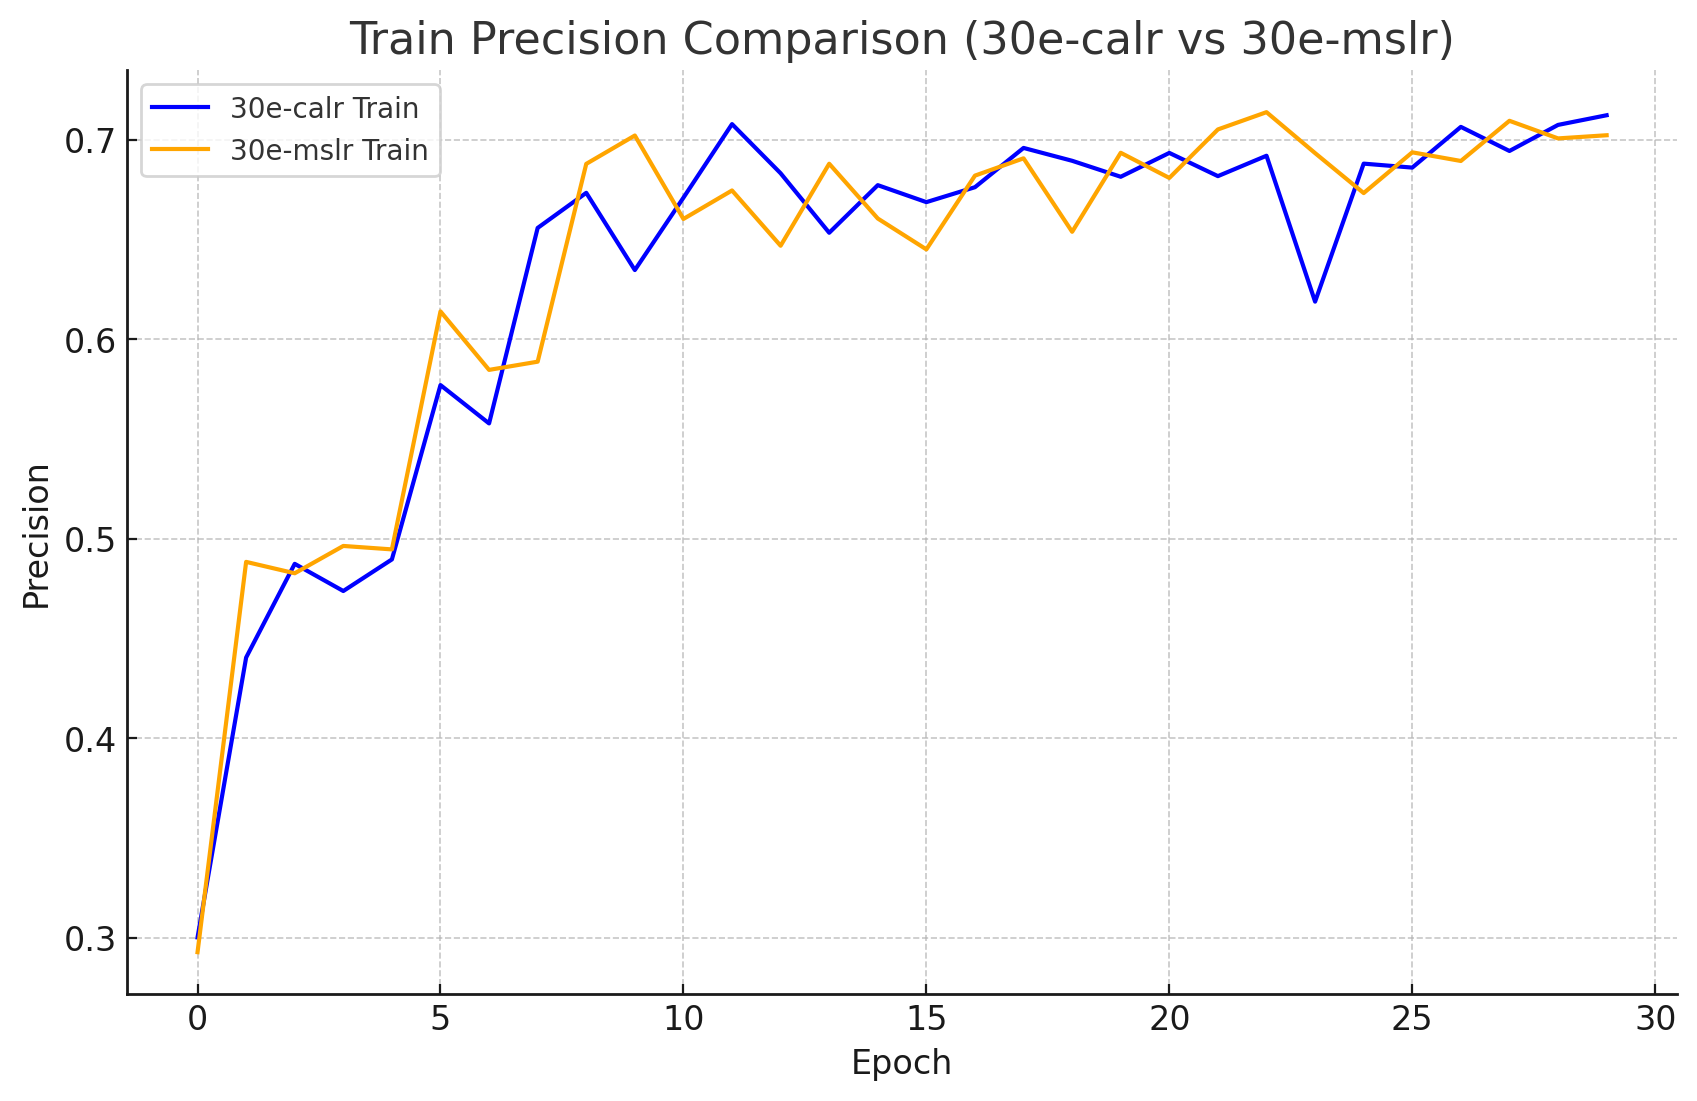
\includegraphics[width=\textwidth]{gambar/bab4-train-precision-30e.png}
    \caption{Precision (training) - 30 \emph{epoch}}
  \end{subfigure}
  \hfill
  \begin{subfigure}{0.45\textwidth}
    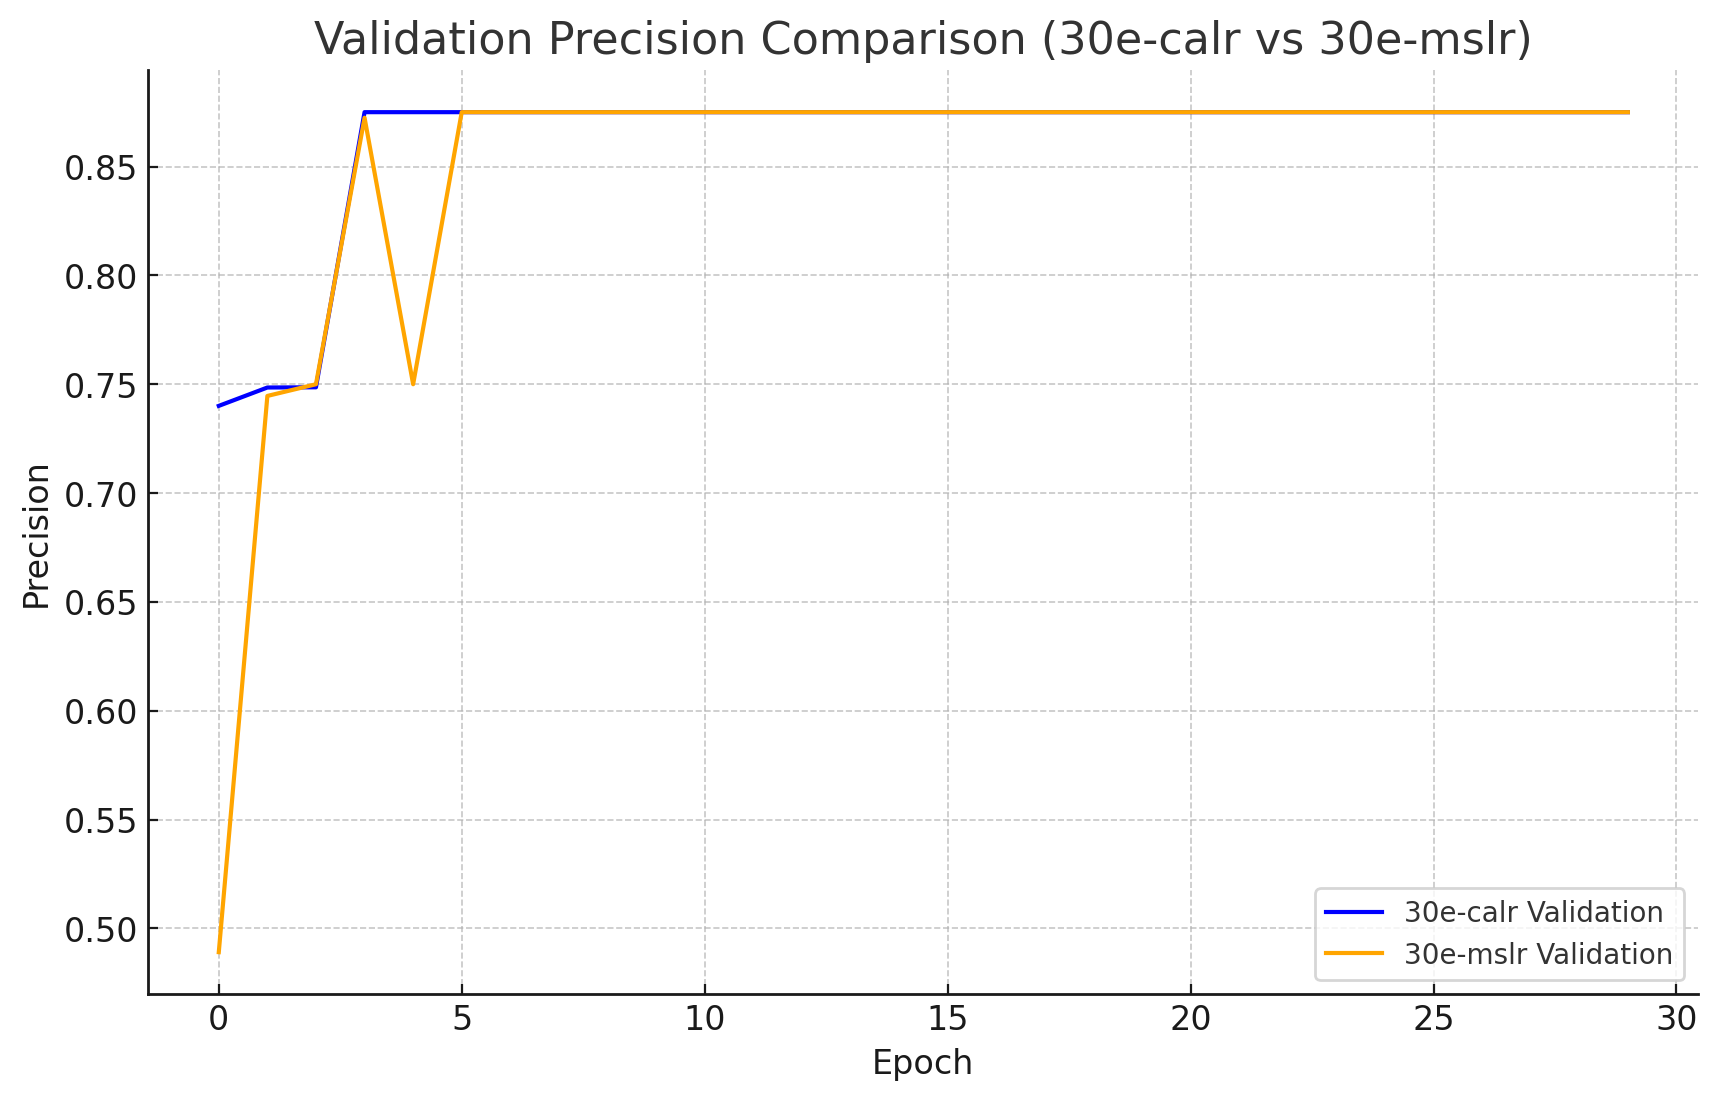
\includegraphics[width=\textwidth]{gambar/bab4-val-precision-30e.png}
    \caption{Precision (validation) - 30 \emph{epoch}}
  \end{subfigure}
  \hfill
  \begin{subfigure}{0.45\textwidth}
    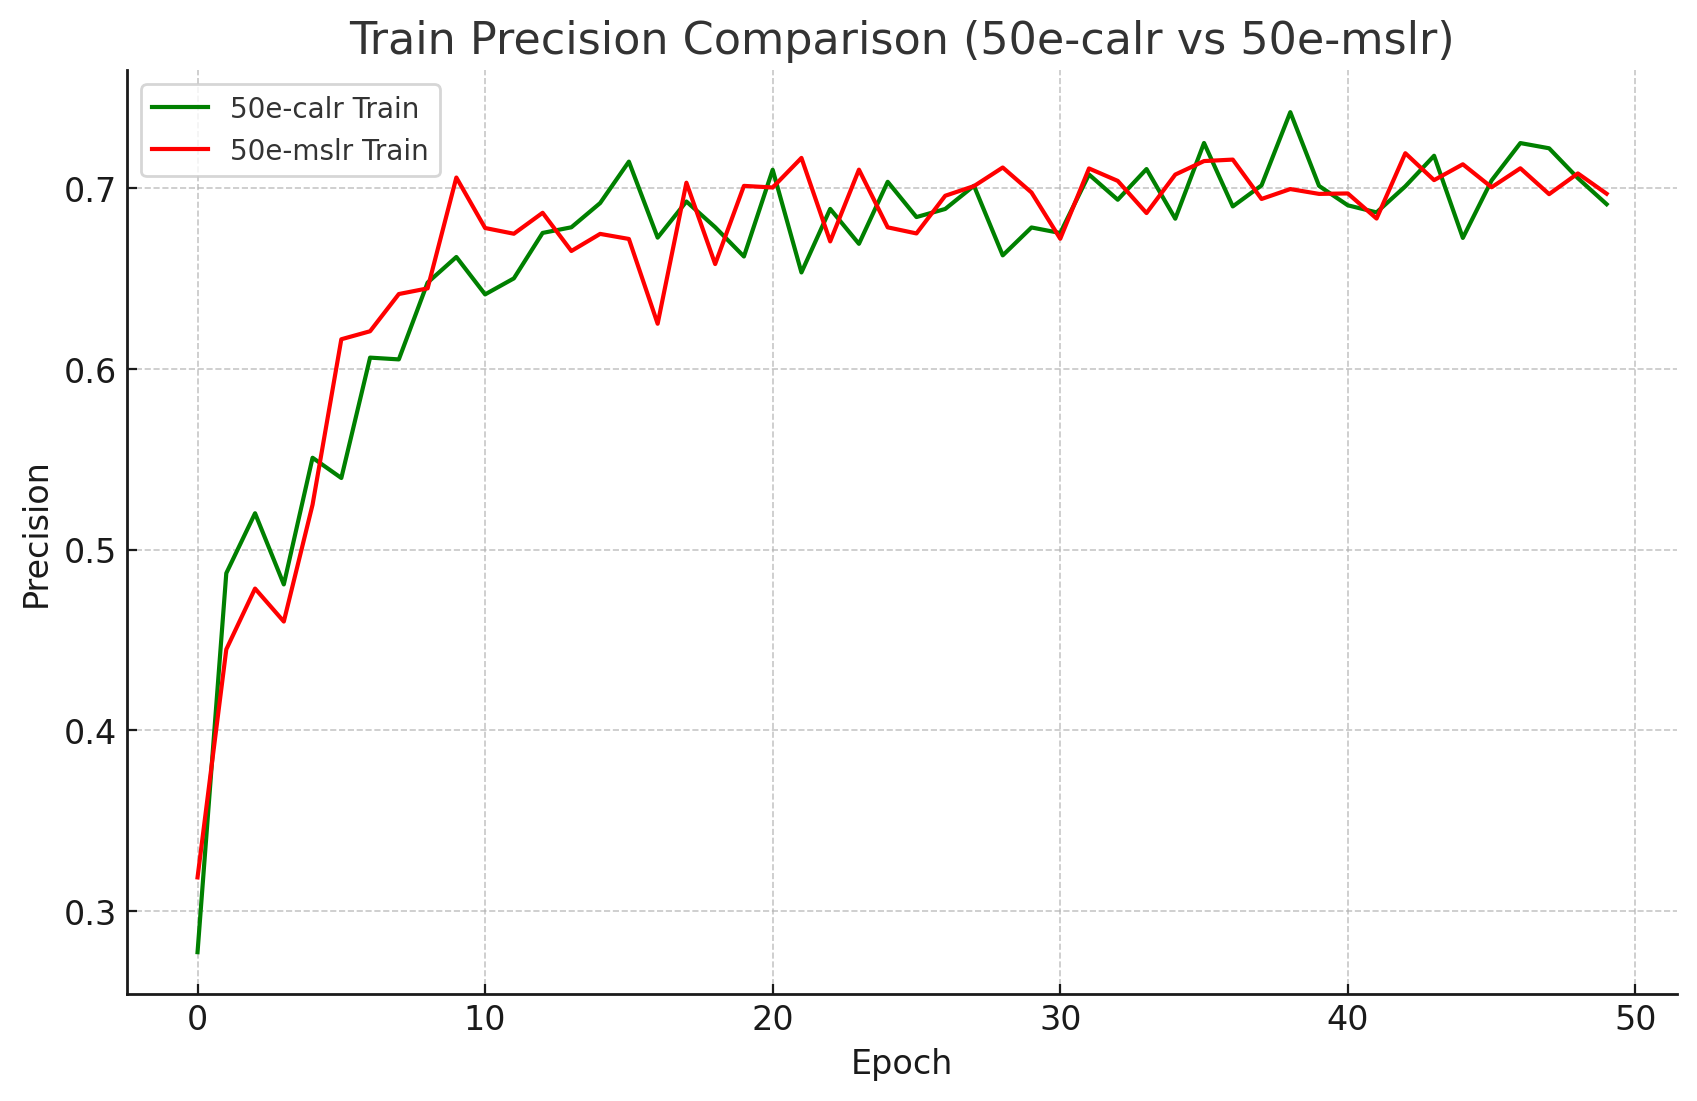
\includegraphics[width=\textwidth]{gambar/bab4-train-precision-50e.png}
    \caption{Precision (training) - 50 \emph{epoch}}
  \end{subfigure}
  \hfill
  \begin{subfigure}{0.45\textwidth}
    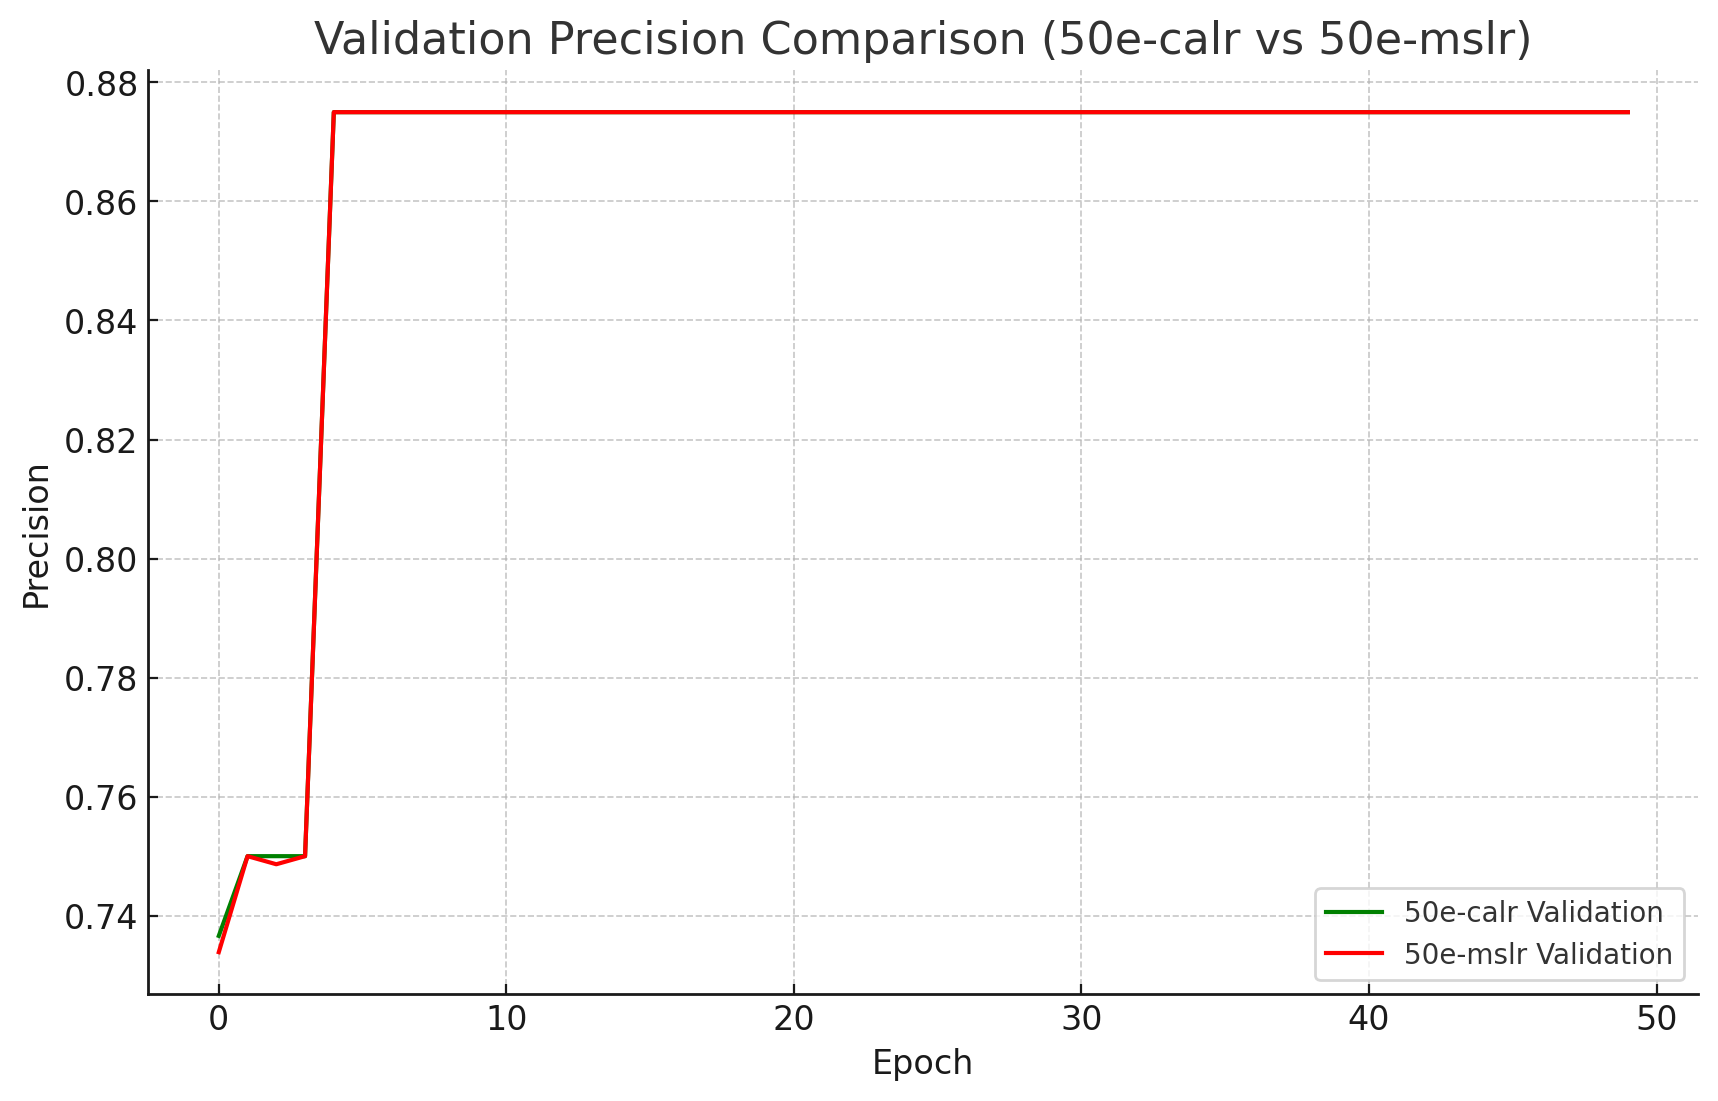
\includegraphics[width=\textwidth]{gambar/bab4-val-precision-50e.png}
    \caption{Precision (validation) - 50 \emph{epoch}}
  \end{subfigure}
  \caption{Kurva Precision selama proses pelatihan model SSD-MobileNetV2}
  \label{fig:precision_curves}
\end{figure}

\begin{figure}[htbp]
  \centering
  \begin{subfigure}{0.45\textwidth}
    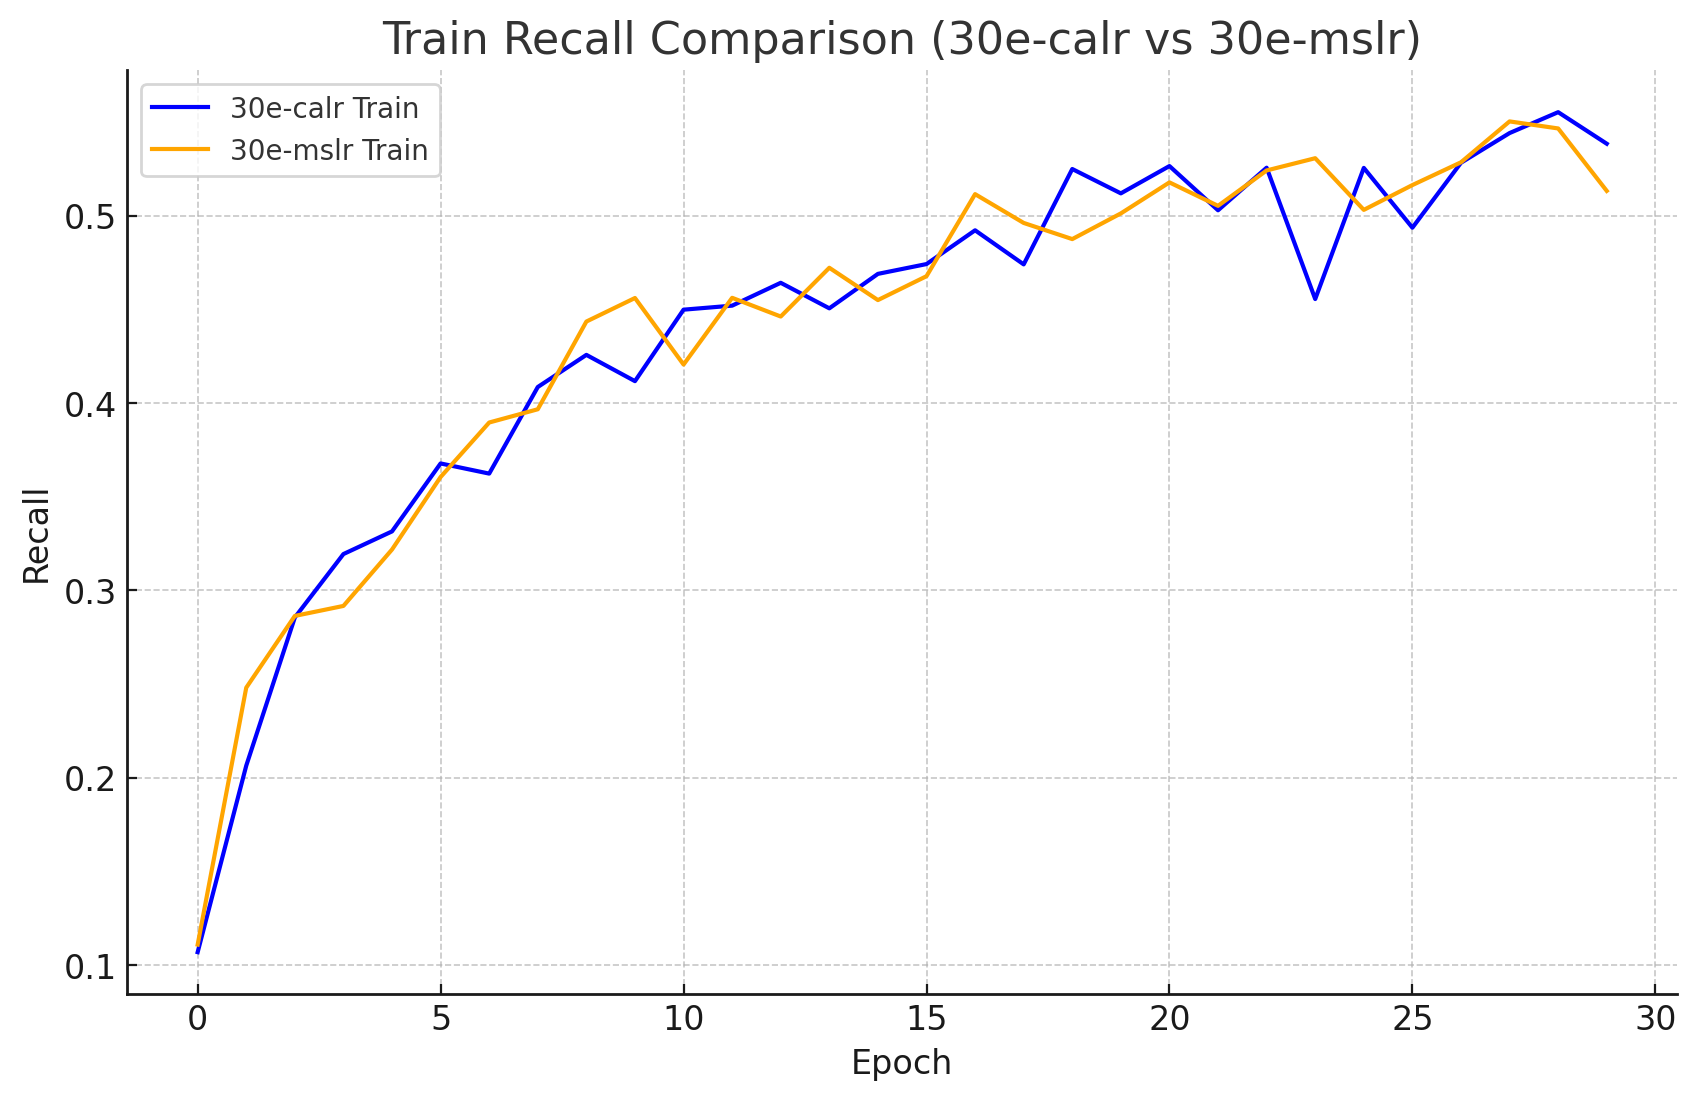
\includegraphics[width=\textwidth]{gambar/bab4-train-recall-30e.png}
    \caption{Recall (training) - 30 \emph{epoch}}
  \end{subfigure}
  \hfill
  \begin{subfigure}{0.45\textwidth}
    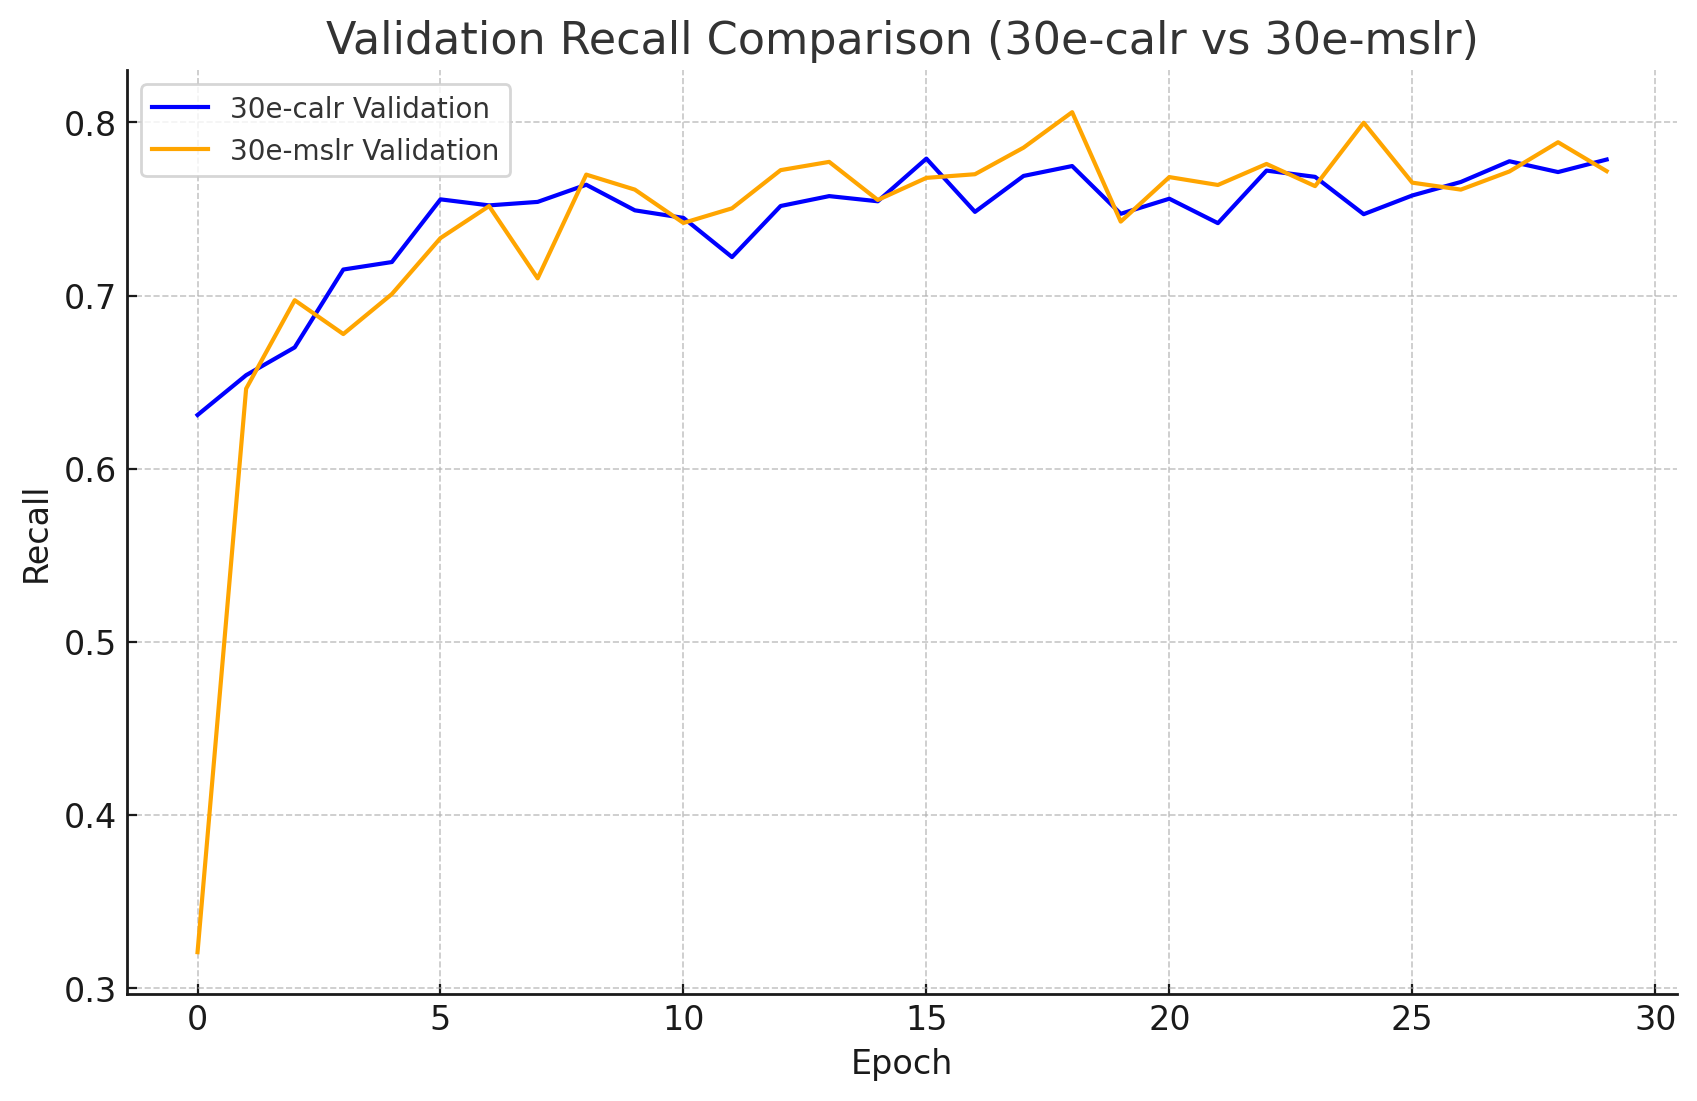
\includegraphics[width=\textwidth]{gambar/bab4-val-recall-30e.png}
    \caption{Recall (validation) - 30 \emph{epoch}}
  \end{subfigure}
  \hfill
  \begin{subfigure}{0.45\textwidth}
    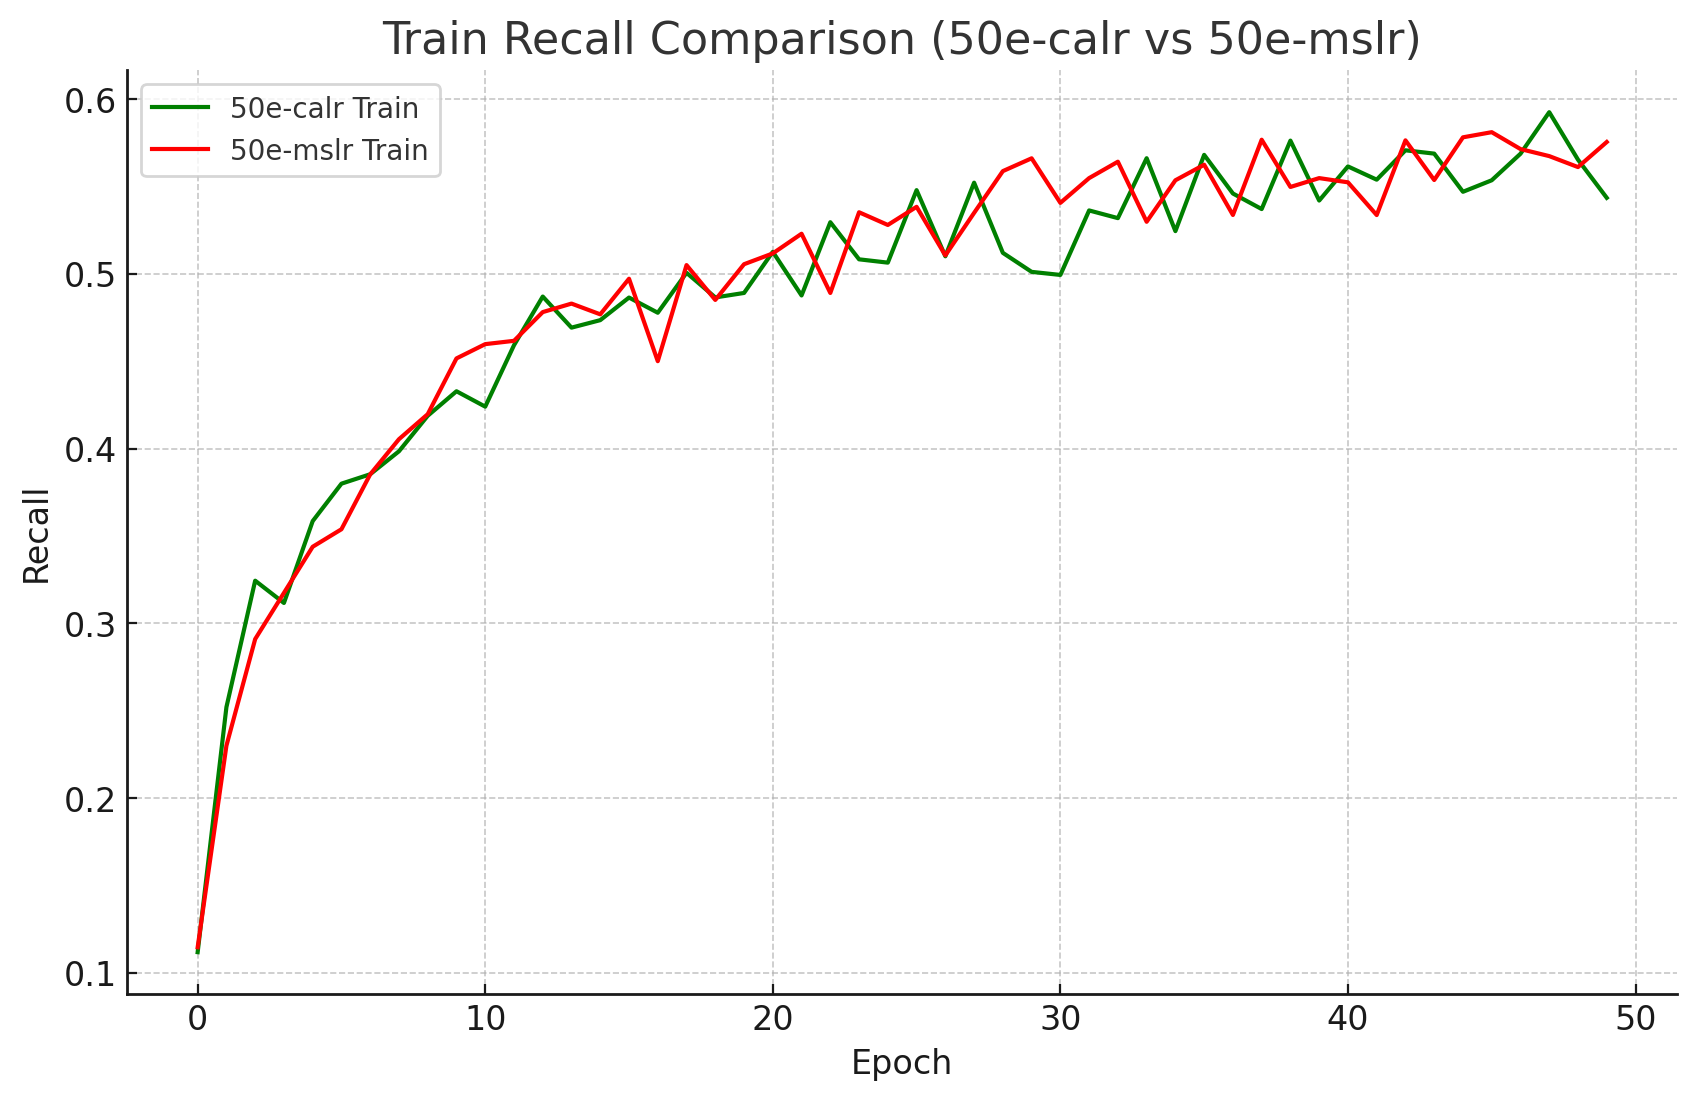
\includegraphics[width=\textwidth]{gambar/bab4-train-recall-50e.png}
    \caption{Recall (training) - 50 \emph{epoch}}
  \end{subfigure}
  \hfill
  \begin{subfigure}{0.45\textwidth}
    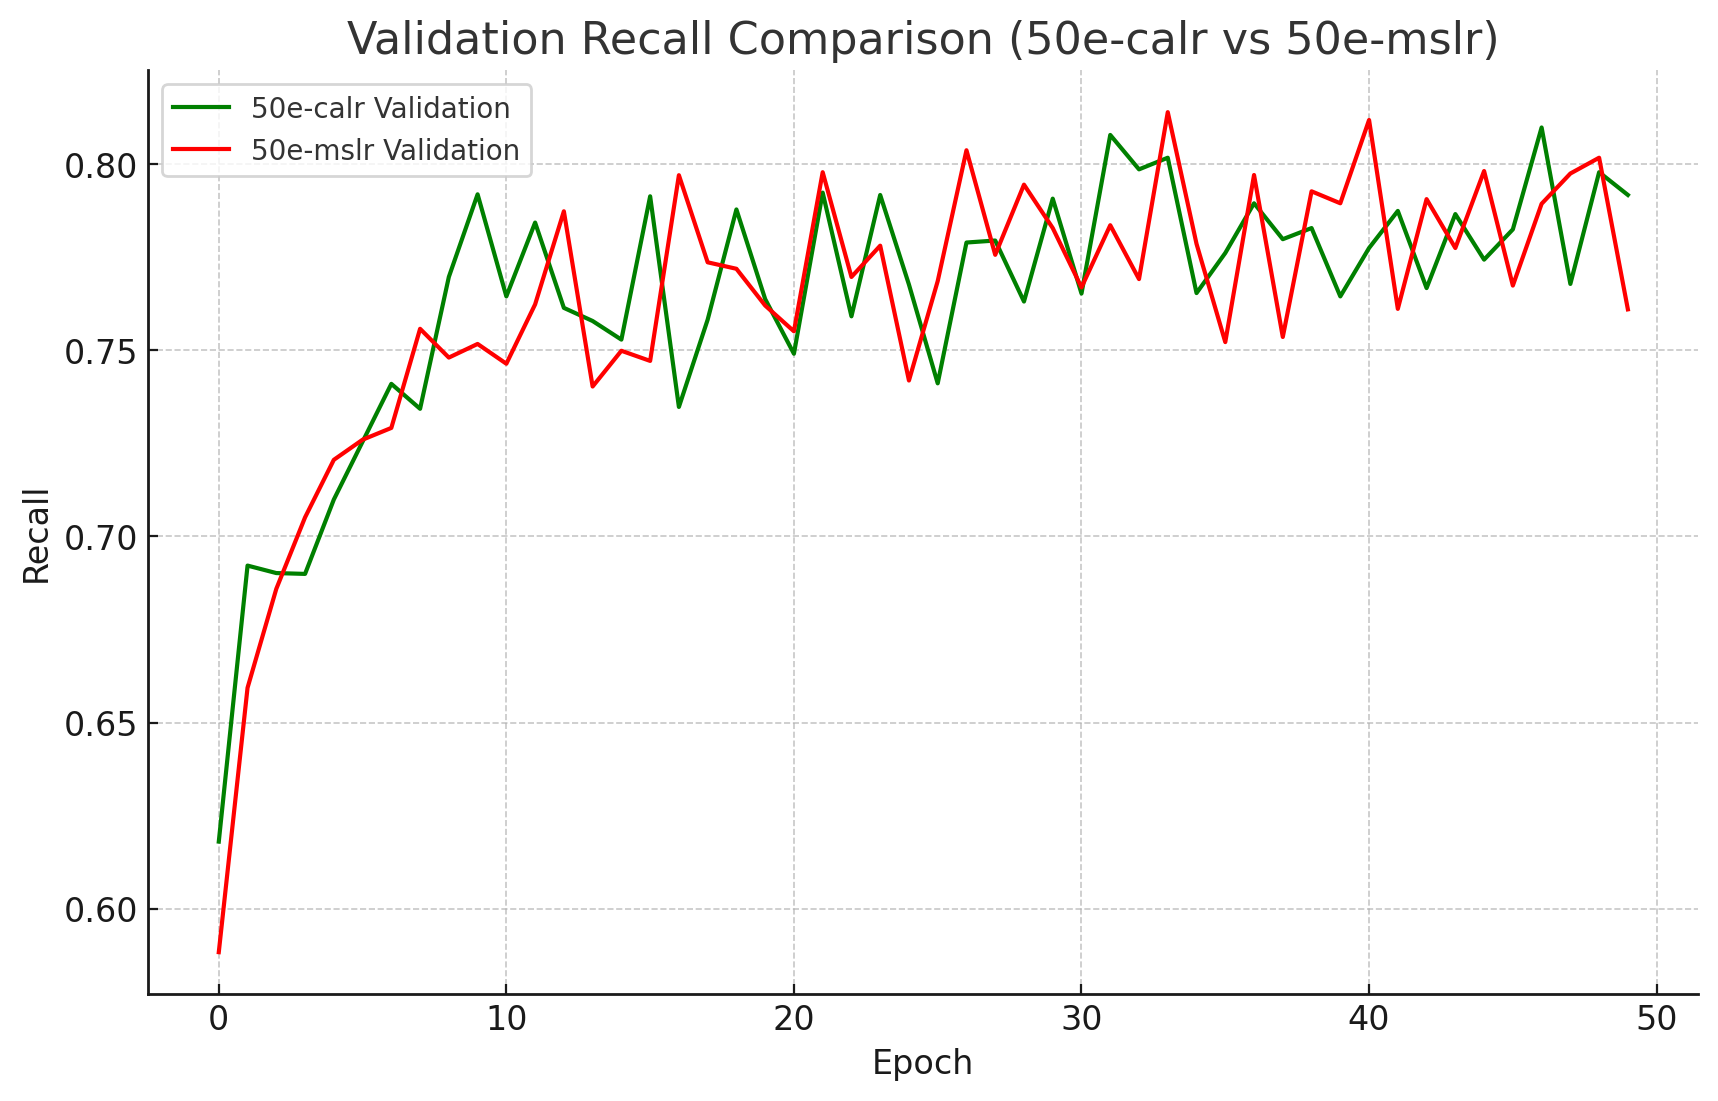
\includegraphics[width=\textwidth]{gambar/bab4-val-recall-50e.png}
    \caption{Recall (validation) - 50 \emph{epoch}}
  \end{subfigure}
  \caption{Kurva Recall selama proses pelatihan model SSD-MobileNetV2}
  \label{fig:recall_curves}
\end{figure}

\begin{figure}[htbp]
  \centering
  \begin{subfigure}{0.45\textwidth}
    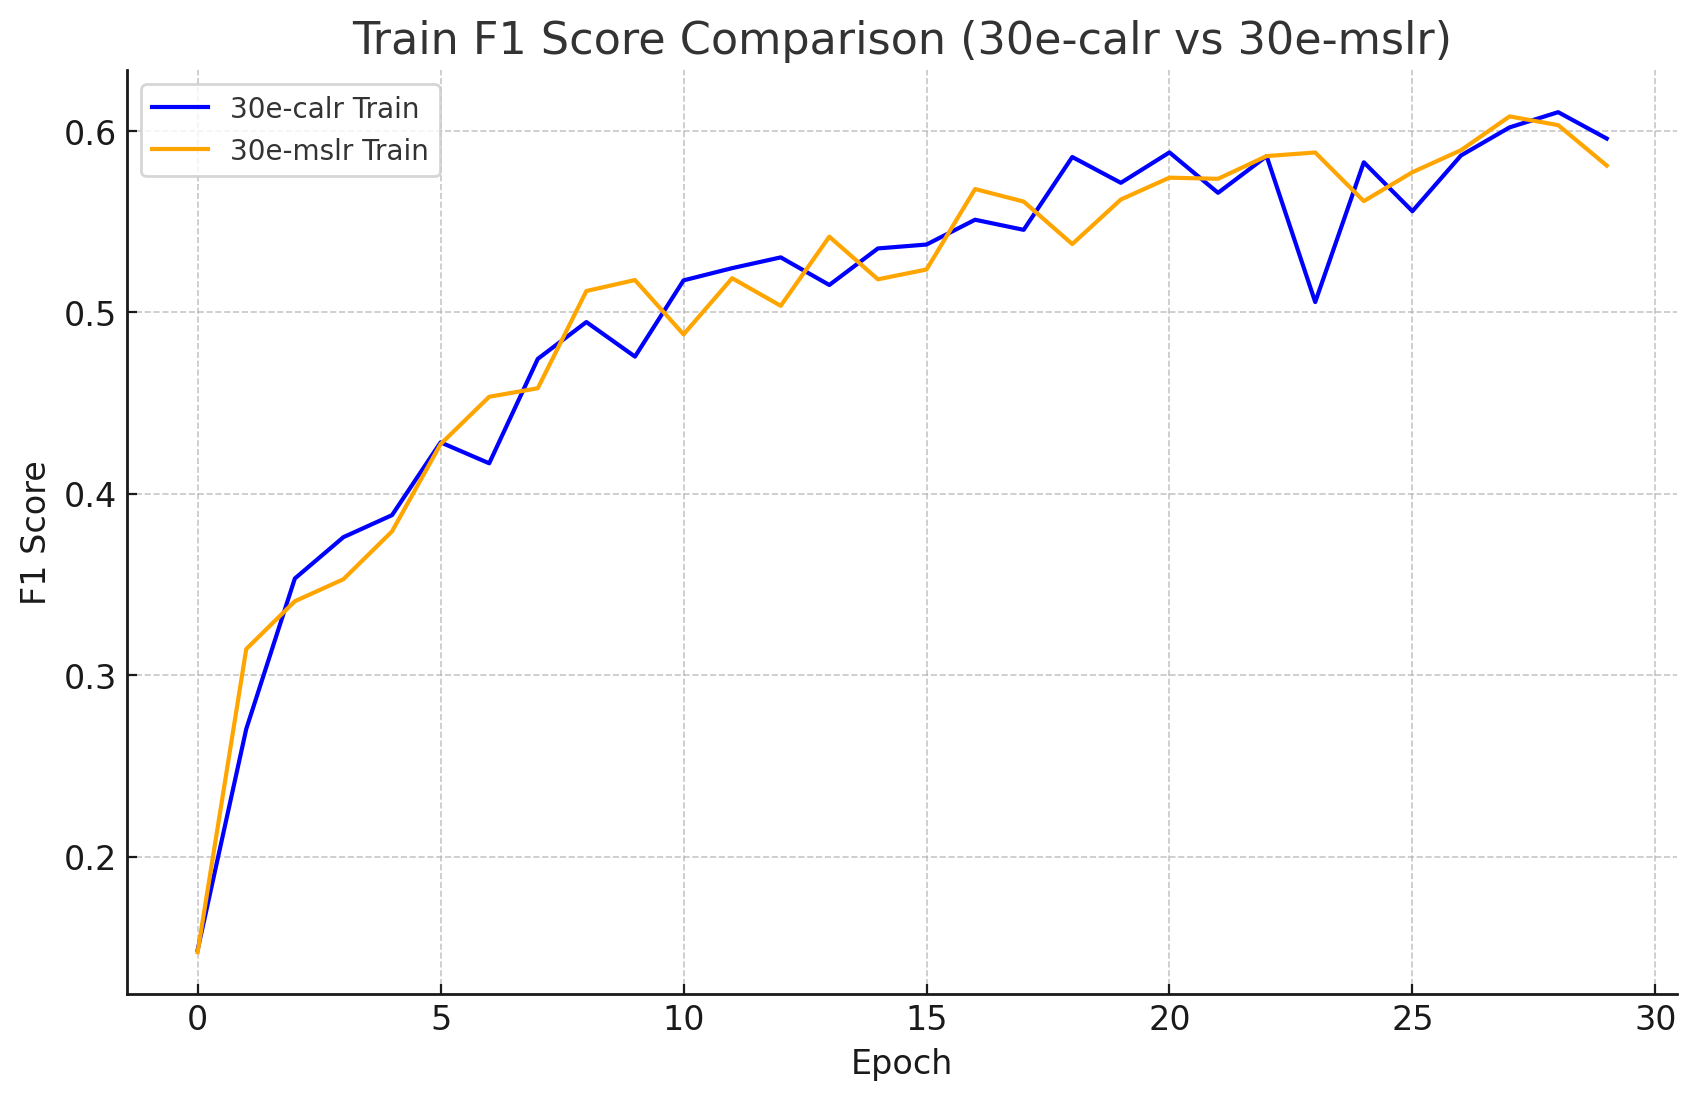
\includegraphics[width=\textwidth]{gambar/bab4-train-f1-score-30e.png}
    \caption{F1 Score (training) - 30 \emph{epoch}}
  \end{subfigure}
  \hfill
  \begin{subfigure}{0.45\textwidth}
    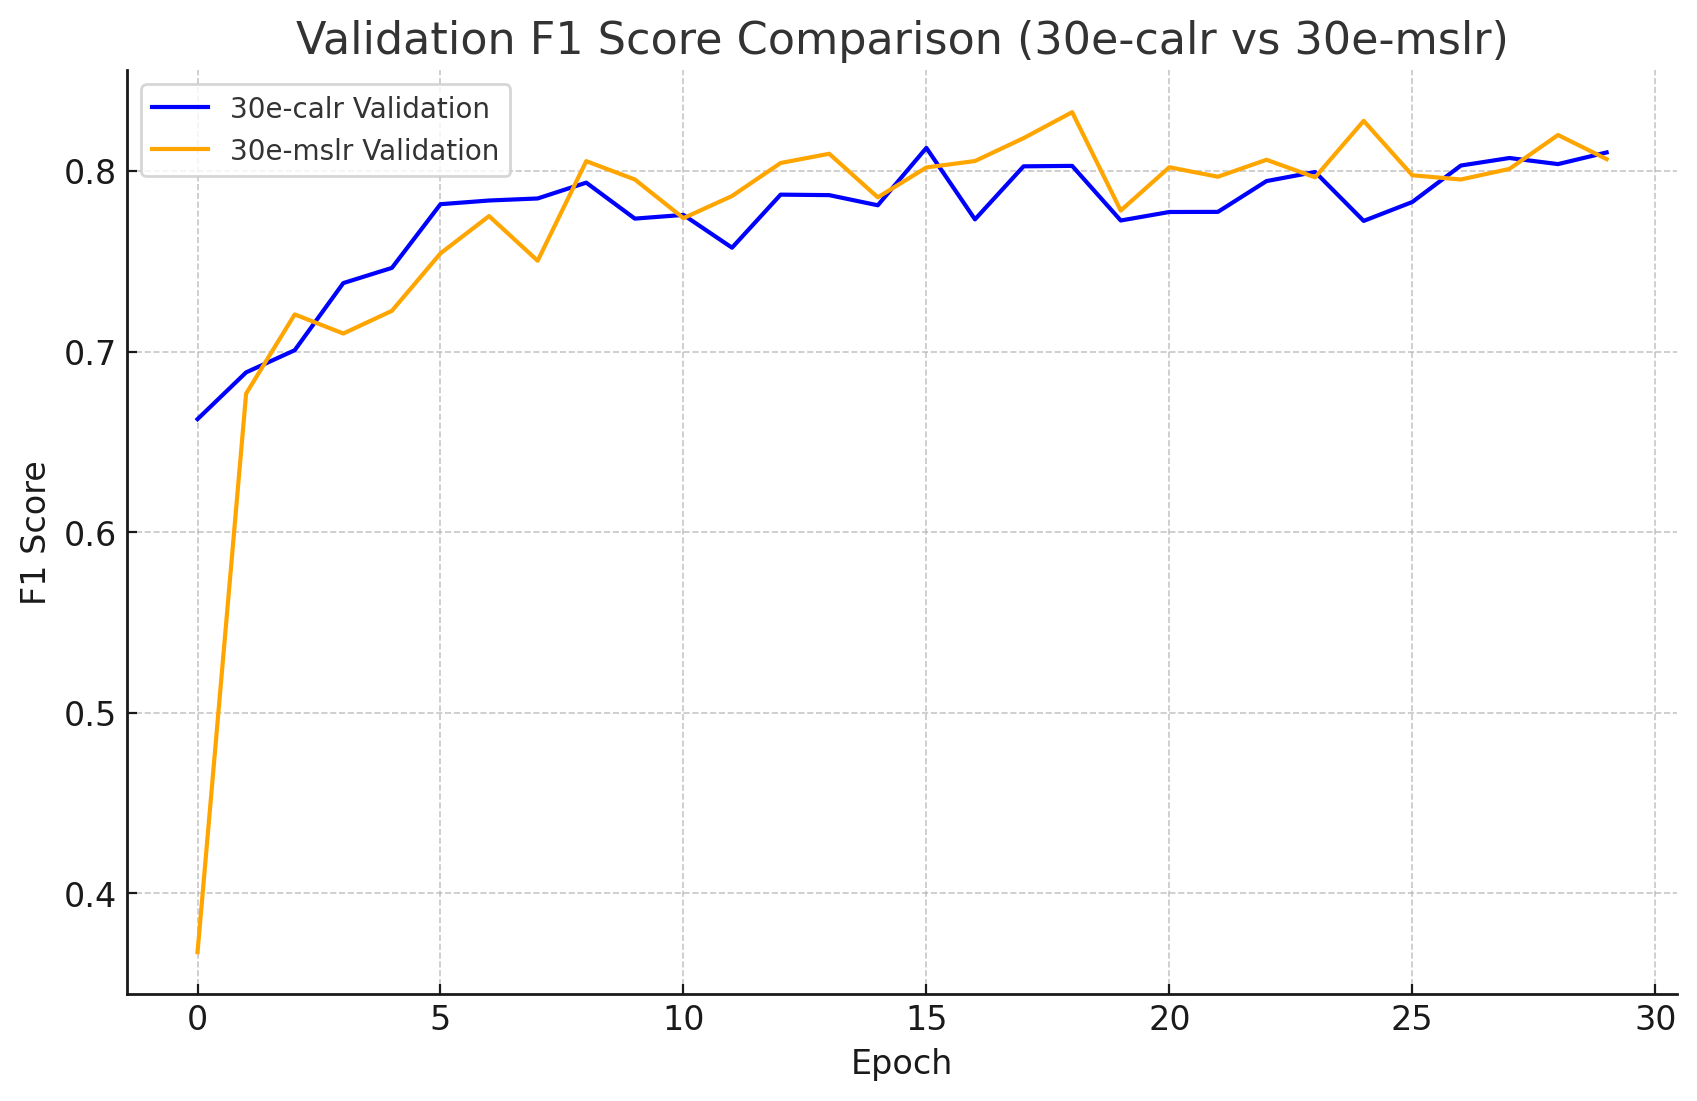
\includegraphics[width=\textwidth]{gambar/bab4-val-f1-score-30e.png}
    \caption{F1 Score (validation) - 30 \emph{epoch}}
  \end{subfigure}
  \hfill
  \begin{subfigure}{0.45\textwidth}
    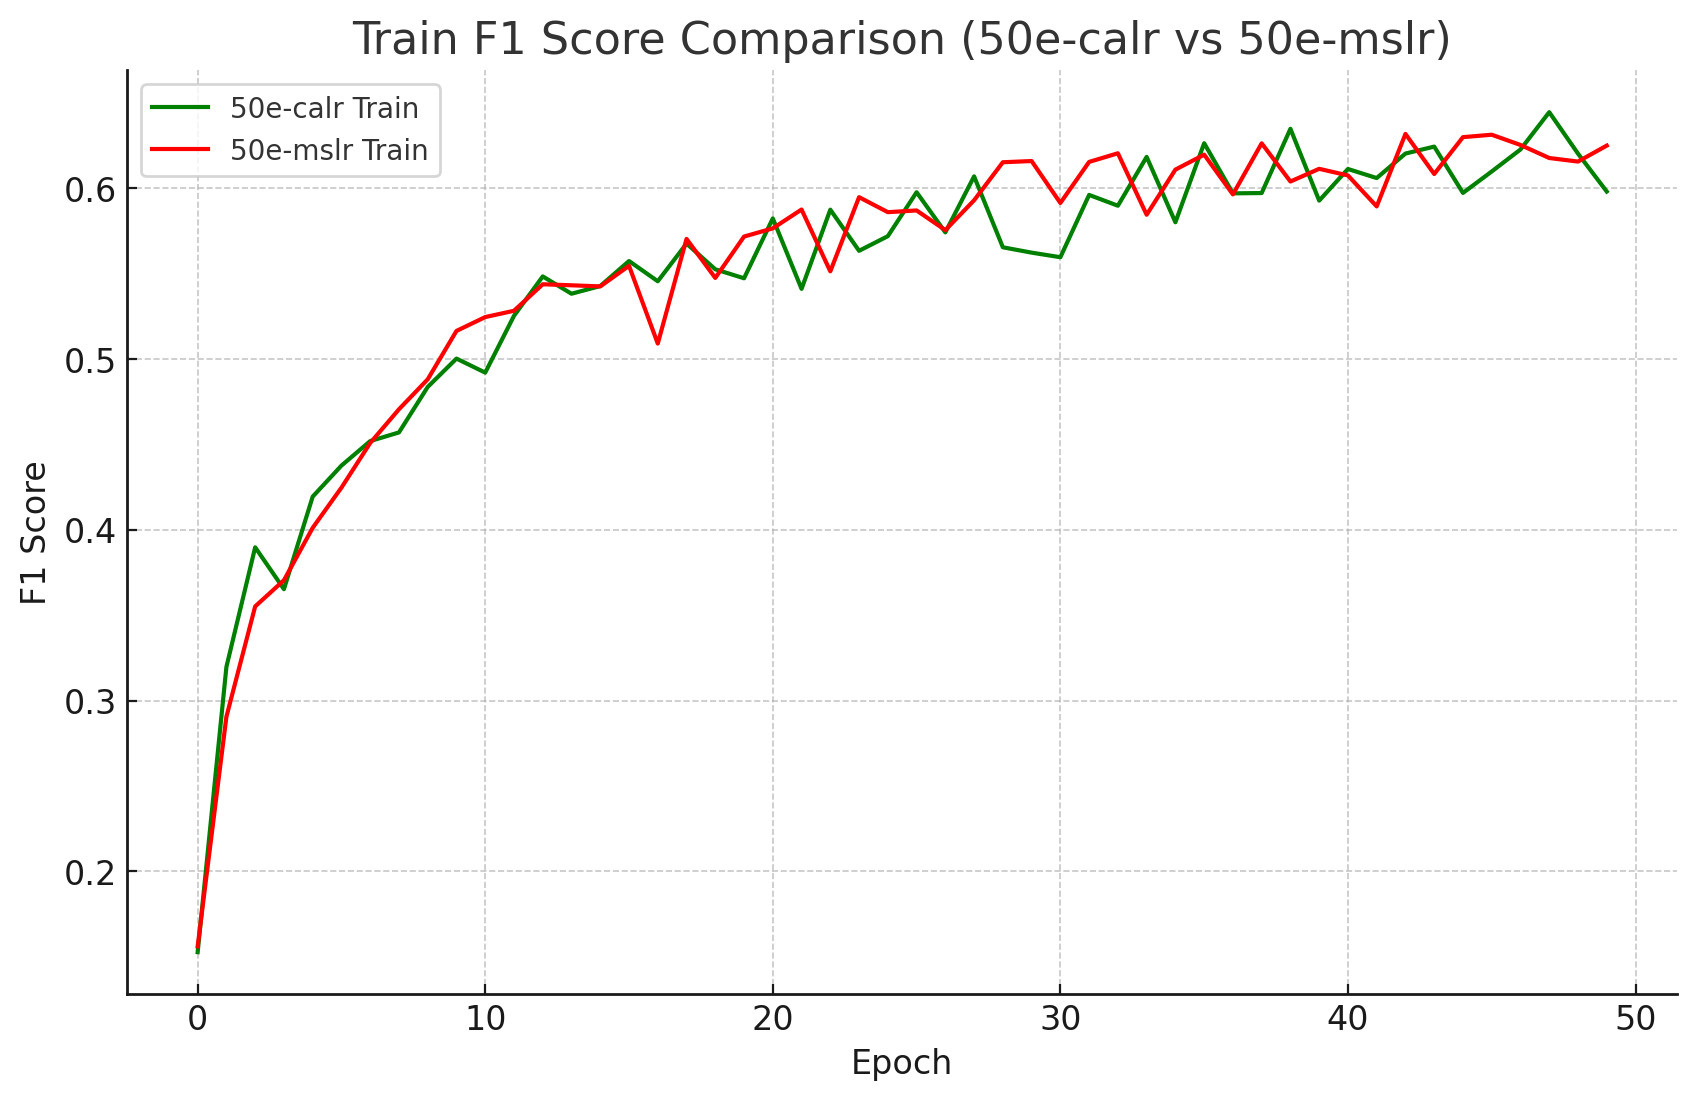
\includegraphics[width=\textwidth]{gambar/bab4-train-f1-score-50e.png}
    \caption{F1 Score (training) - 50 \emph{epoch}}
  \end{subfigure}
  \hfill
  \begin{subfigure}{0.45\textwidth}
    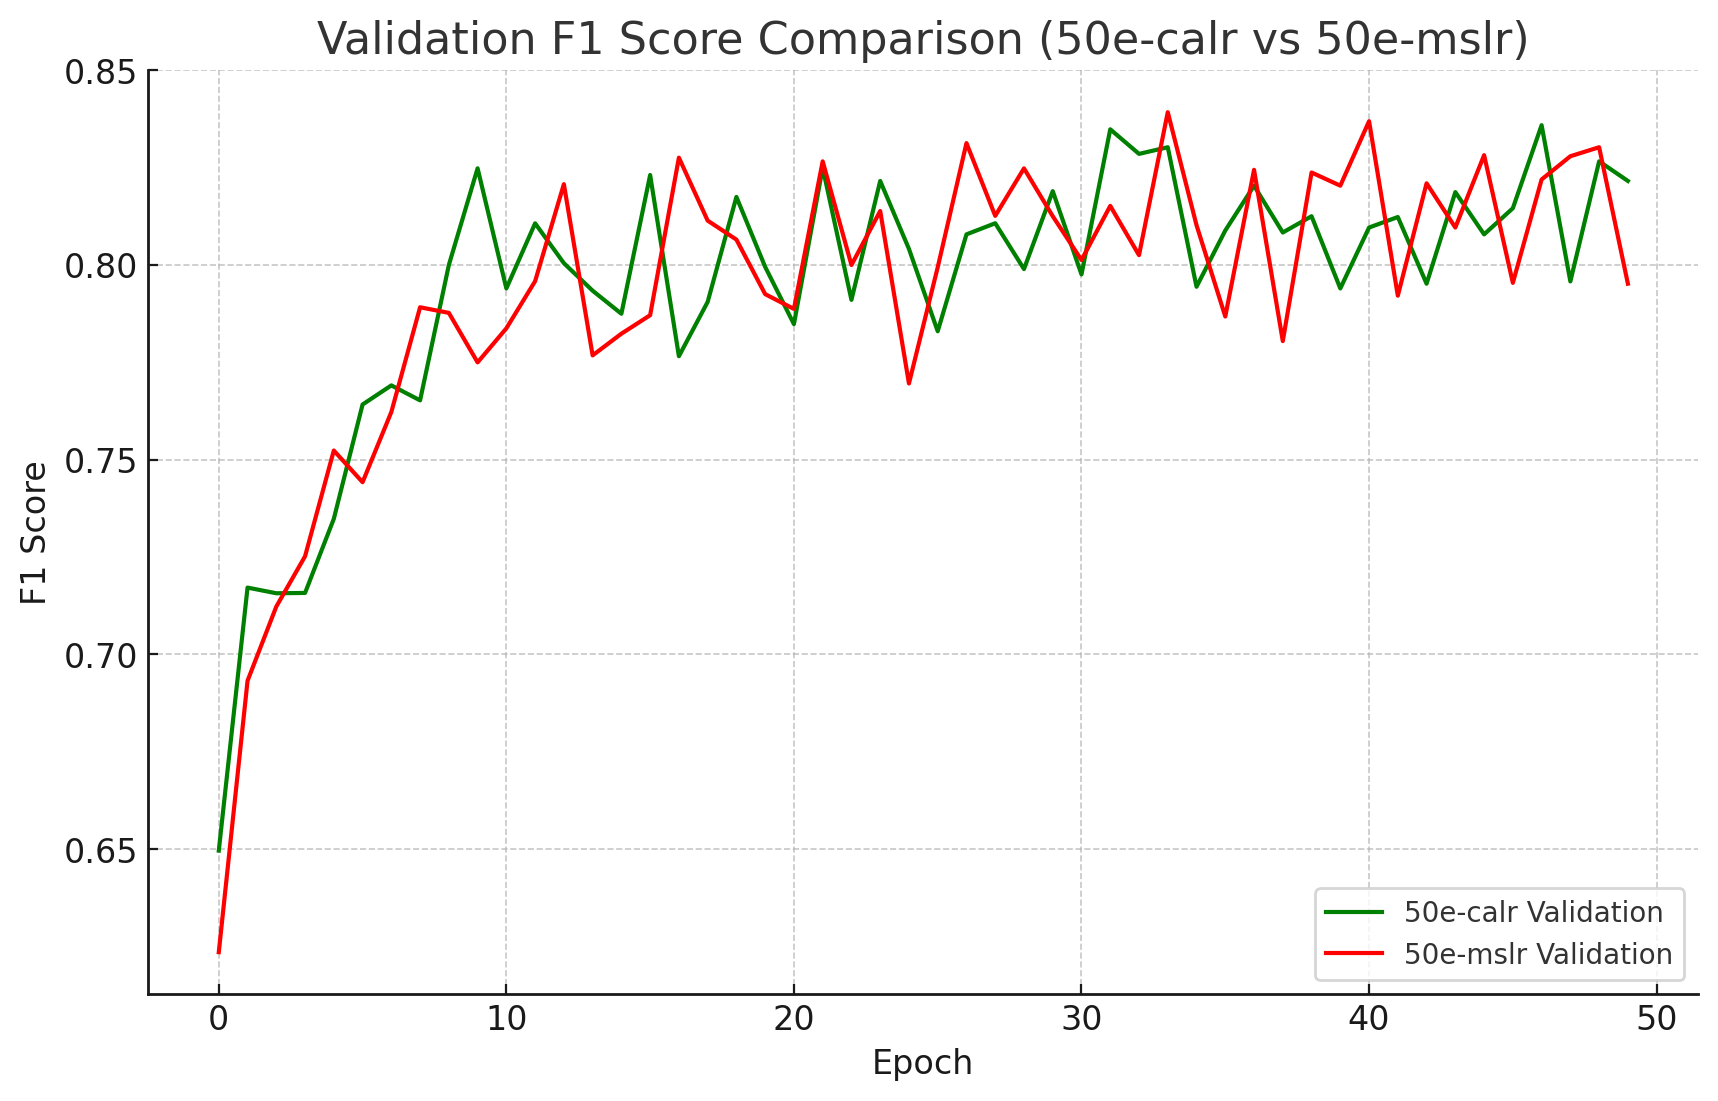
\includegraphics[width=\textwidth]{gambar/bab4-val-f1-score-50e.png}
    \caption{F1 Score (validation) - 50 \emph{epoch}}
  \end{subfigure}
  \caption{Kurva F1 Score selama proses pelatihan model SSD-MobileNetV2}
  \label{fig:f1_score_curves}
\end{figure}

\begin{figure}[htbp]
  \centering
  \begin{subfigure}{0.45\textwidth}
    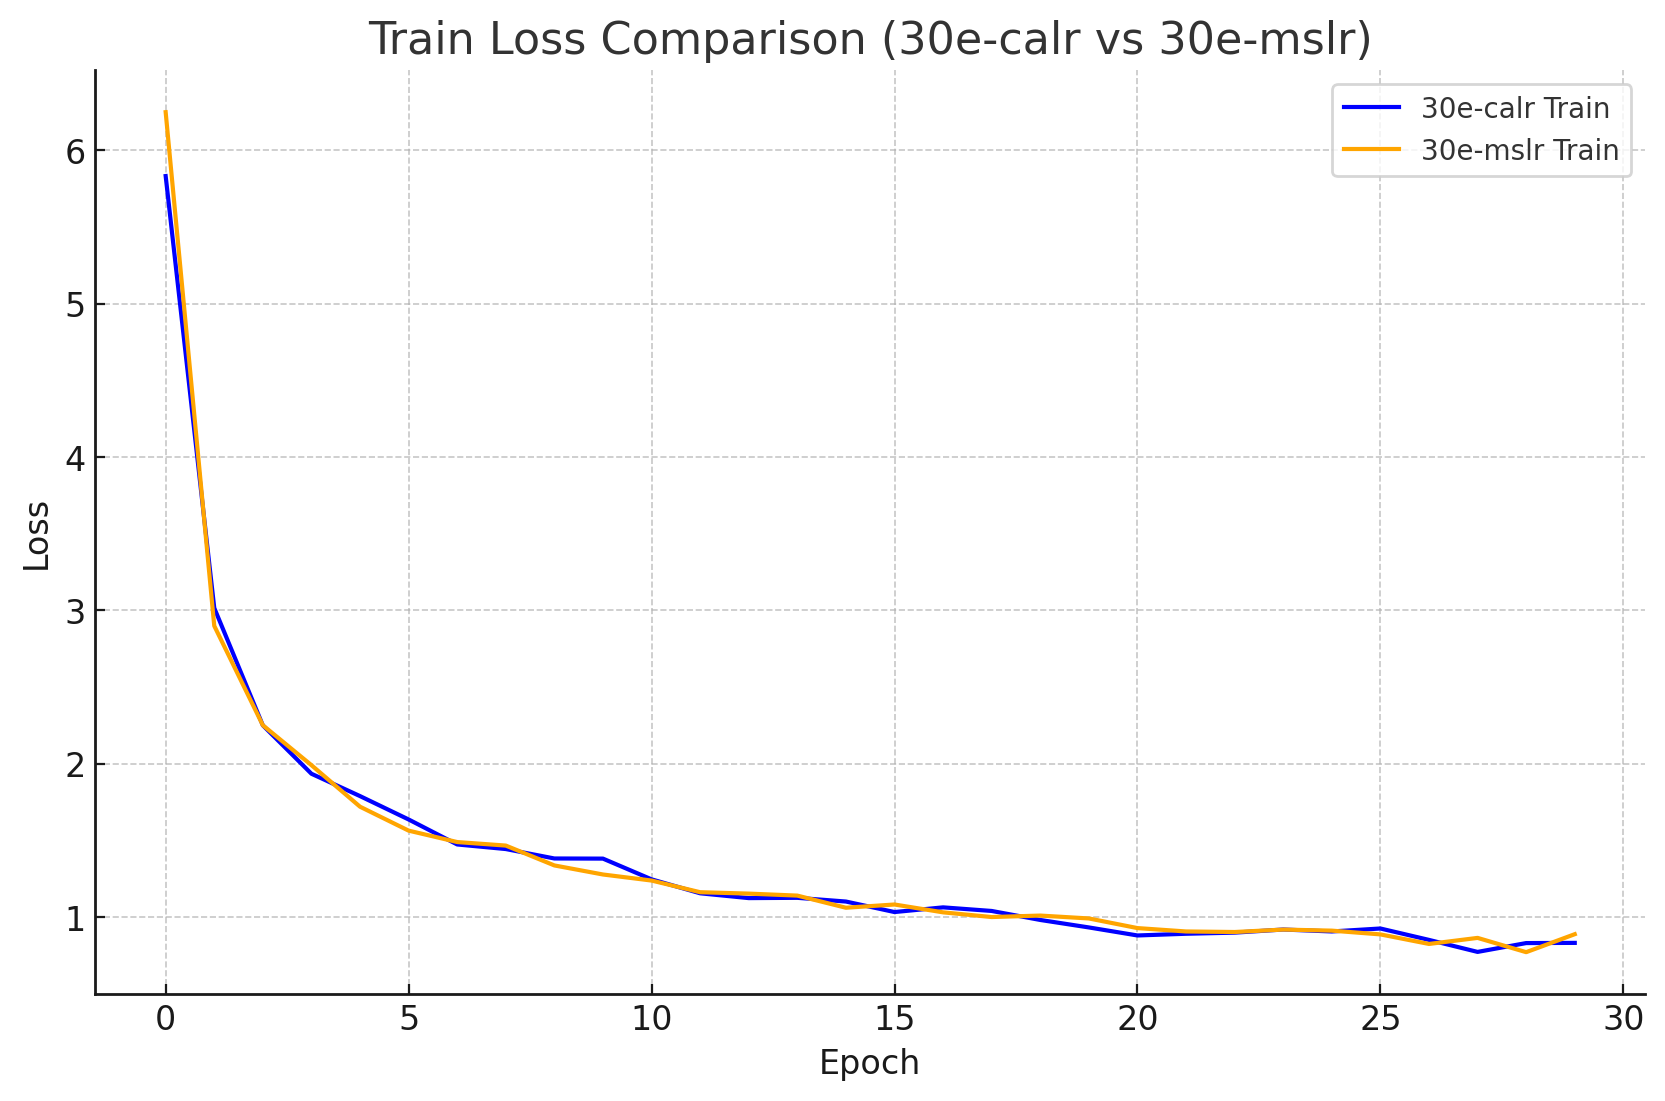
\includegraphics[width=\textwidth]{gambar/bab4-train-loss-30e.png}
    \caption{Loss (training) - 30 \emph{epoch}}
  \end{subfigure}
  \hfill
  \begin{subfigure}{0.45\textwidth}
    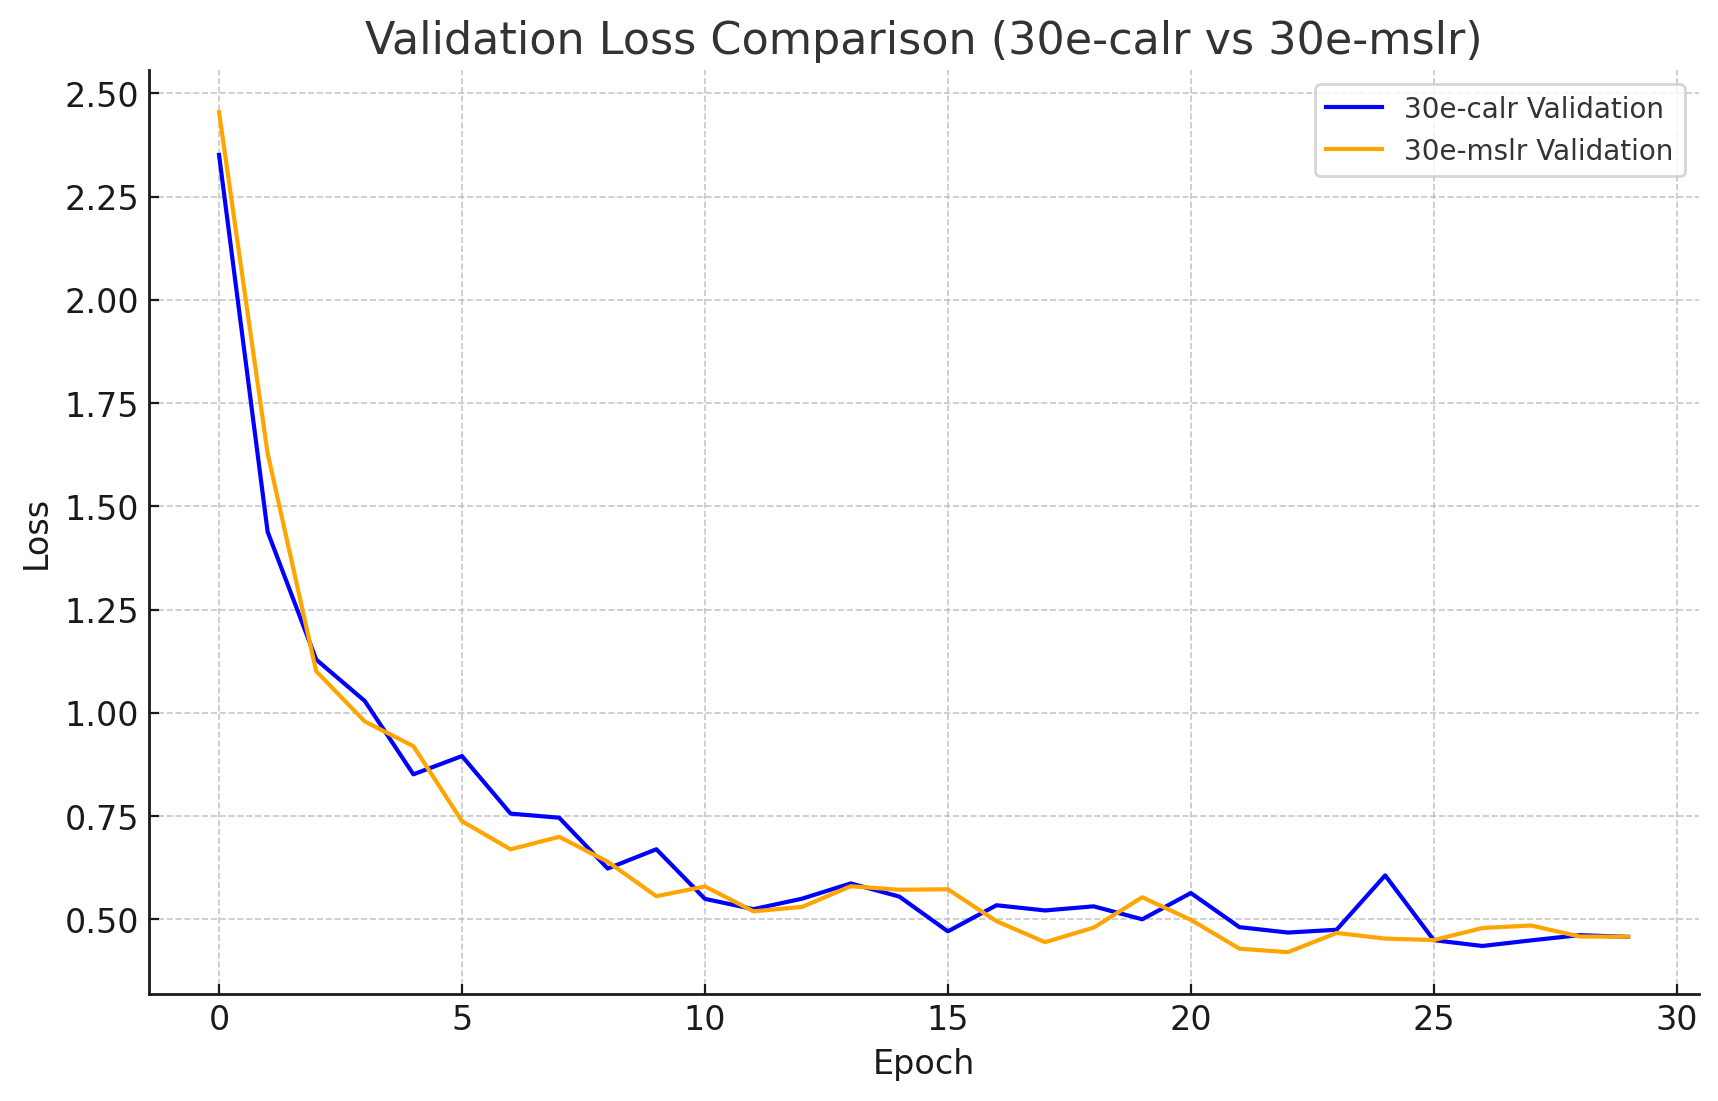
\includegraphics[width=\textwidth]{gambar/bab4-val-loss-30e.png}
    \caption{Loss (validation) - 30 \emph{epoch}}
  \end{subfigure}
  \hfill
  \begin{subfigure}{0.45\textwidth}
    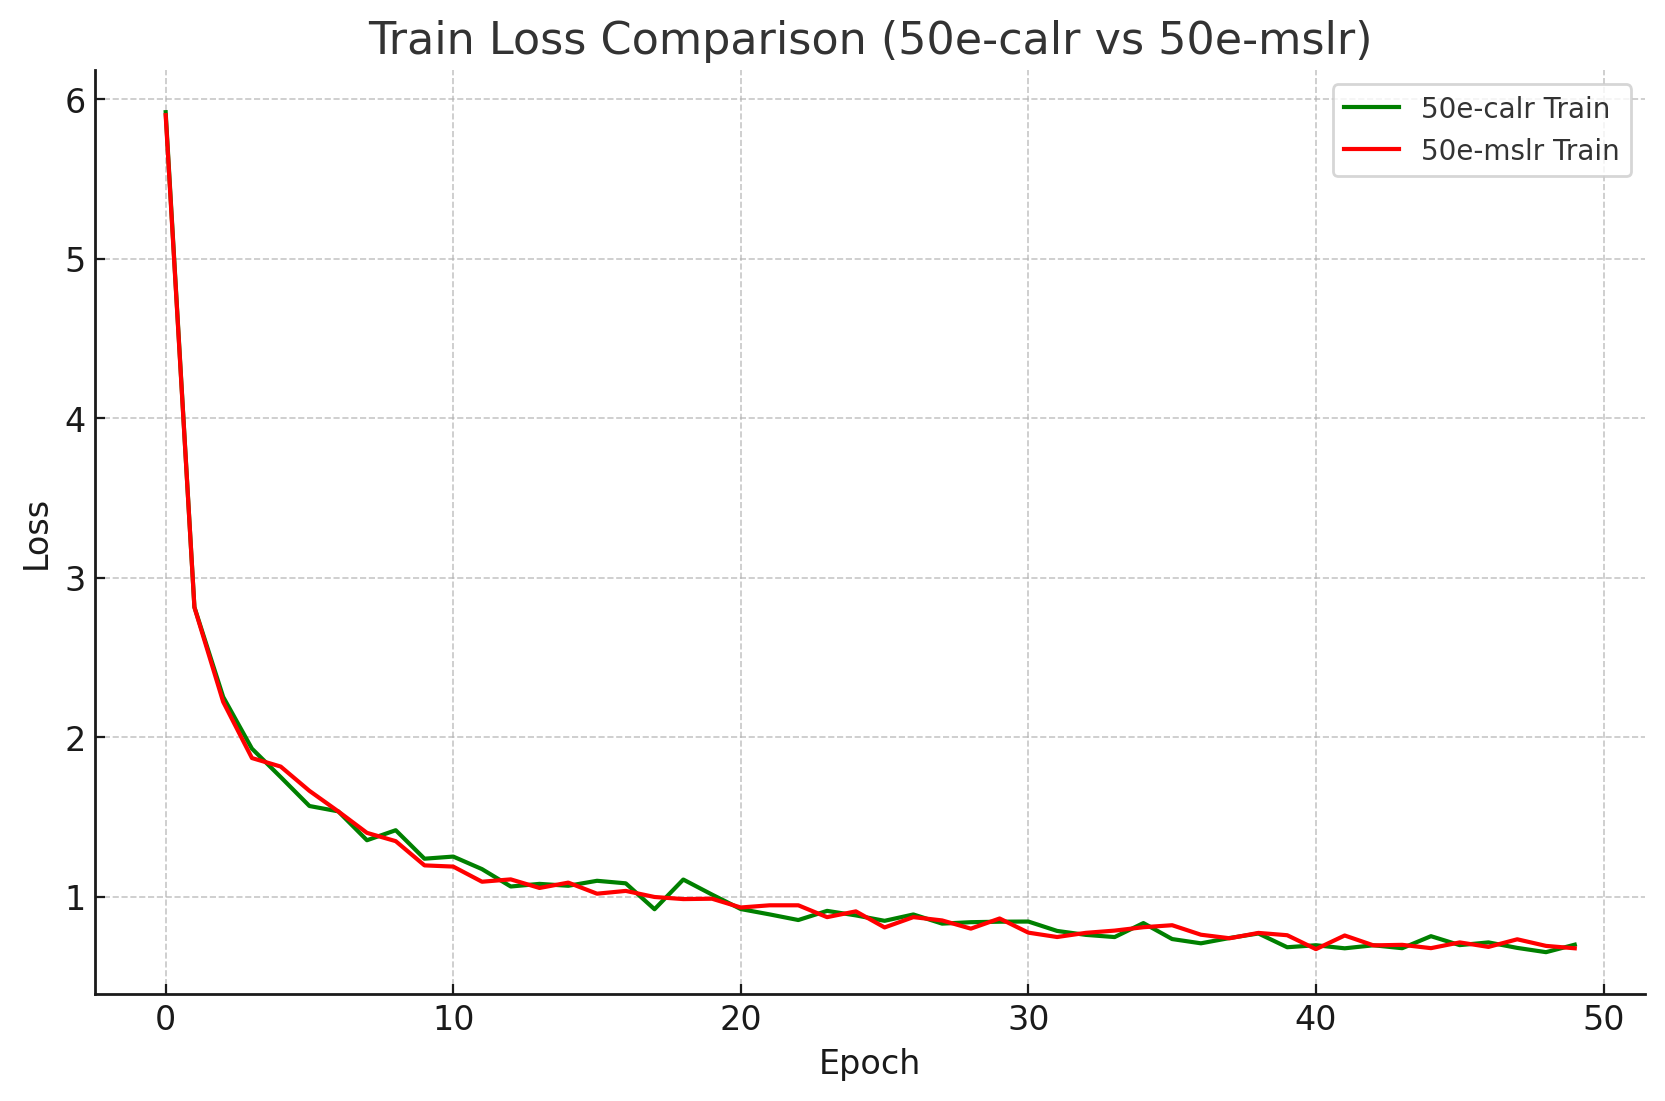
\includegraphics[width=\textwidth]{gambar/bab4-train-loss-50e.png}
    \caption{Loss (training) - 50 \emph{epoch}}
  \end{subfigure}
  \hfill
  \begin{subfigure}{0.45\textwidth}
    \includegraphics[width=\textwidth]{gambar/bab4-val-loss-50e.png}
    \caption{Loss (validation) - 50 \emph{epoch}}
  \end{subfigure}
  \caption{Kurva Loss selama proses pelatihan model SSD-MobileNetV2}
  \label{fig:loss_curves}
\end{figure}

\begin{figure}[htbp]
  \centering
  \begin{subfigure}{0.45\textwidth}
    \includegraphics[width=\textwidth]{gambar/bab4-train-clsloss-30e.png}
    \caption{Classification Loss (training) - 30 \emph{epoch}}
  \end{subfigure}
  \hfill
  \begin{subfigure}{0.45\textwidth}
    \includegraphics[width=\textwidth]{gambar/bab4-val-clsloss-30e.png}
    \caption{Classification Loss (validation) - 30 \emph{epoch}}
  \end{subfigure}
  \hfill
  \begin{subfigure}{0.45\textwidth}
    \includegraphics[width=\textwidth]{gambar/bab4-train-clsloss-50e.png}
    \caption{Classification Loss (training) - 50 \emph{epoch}}
  \end{subfigure}
  \hfill
  \begin{subfigure}{0.45\textwidth}
    \includegraphics[width=\textwidth]{gambar/bab4-val-clsloss-50e.png}
    \caption{Classification Loss (validation) - 50 \emph{epoch}}
  \end{subfigure}
  \caption{Kurva Classification Loss selama proses pelatihan model SSD-MobileNetV2}
  \label{fig:classification_loss_curves}
\end{figure}

\begin{figure}[htbp]
  \centering
  \begin{subfigure}{0.45\textwidth}
    \includegraphics[width=\textwidth]{gambar/bab4-train-regloss-30e.png}
    \caption{Regression Loss (training) - 30 \emph{epoch}}
  \end{subfigure}
  \hfill
  \begin{subfigure}{0.45\textwidth}
    \includegraphics[width=\textwidth]{gambar/bab4-val-regloss-30e.png}
    \caption{Regression Loss (validation) - 30 \emph{epoch}}
  \end{subfigure}
  \hfill
  \begin{subfigure}{0.45\textwidth}
    \includegraphics[width=\textwidth]{gambar/bab4-train-regloss-50e.png}
    \caption{Regression Loss (training) - 50 \emph{epoch}}
  \end{subfigure}
  \hfill
  \begin{subfigure}{0.45\textwidth}
    \includegraphics[width=\textwidth]{gambar/bab4-val-regloss-50e.png}
    \caption{Regression Loss (validation) - 50 \emph{epoch}}
  \end{subfigure}
  \caption{Kurva Regression Loss selama proses pelatihan model SSD-MobileNetV2}
  \label{fig:regression_loss_curves}
\end{figure}      

Berdasarkan grafik yang ditampilkan pada gambar \ref{fig:accuracy_curves}, \ref{fig:precision_curves}, \ref{fig:recall_curves}, \ref{fig:f1_score_curves}, \ref{fig:loss_curves}, \ref{fig:classification_loss_curves}, dan \ref{fig:regression_loss_curves}, dapat dianalisis hasil pelatihan dari empat konfigurasi model yang berbeda, yaitu 30 \emph{epoch} dengan \emph{scheduler} \emph{CosineAnnealingLR}, 30 \emph{epoch} dengan \emph{scheduler} \emph{MultiStepLR}, 50 \emph{epoch} dengan \emph{scheduler} \emph{CosineAnnealingLR}, dan 50 \emph{epoch} dengan \emph{scheduler} \emph{MultiStepLR}.

Secara umum, tren yang terlihat pada grafik adalah penurunan loss yang stabil dan akurasi yang meningkat seiring dengan penambahan \emph{epoch}. Namun, terdapat beberapa perbedaan yang mencolok antara konfigurasi yang satu dengan yang lainnya.

\subsubsection{30 \emph{epoch} dengan \emph{CosineAnnealingLR} vs \emph{MultiStepLR}}

Pada grafik \ref{fig:accuracy_curves}, terlihat bahwa konfigurasi 30 \emph{epoch} dengan \emph{CosineAnnealingLR} (\emph{30e-calr}) menunjukkan peningkatan akurasi yang lebih cepat dibandingkan dengan konfigurasi 30 \emph{epoch} dengan \emph{MultiStepLR} (\emph{30e-mslr}) pada awal pelatihan. Namun, setelah mencapai titik tertentu, kedua konfigurasi tersebut mulai mendekati hasil yang serupa pada \emph{epoch} akhir. 

Pada grafik \ref{fig:loss_curves}, kita juga dapat melihat bahwa \emph{30e-calr} cenderung memiliki penurunan loss yang lebih stabil, sementara \emph{30e-mslr} menunjukkan fluktuasi yang lebih besar terutama pada \emph{epoch} awal. Meskipun demikian, kedua konfigurasi mengalami penurunan loss yang cukup signifikan sepanjang pelatihan.

\subsubsection{50 \emph{epoch} dengan \emph{CosineAnnealingLR} vs \emph{MultiStepLR}}

Untuk konfigurasi 50 \emph{epoch}, pada grafik \ref{fig:accuracy_curves} dan \ref{fig:loss_curves}, terlihat bahwa konfigurasi 50 \emph{epoch} dengan \emph{CosineAnnealingLR} (\emph{50e-calr}) dan \emph{50e-mslr} menunjukkan tren yang lebih stabil dibandingkan dengan konfigurasi 30 \emph{epoch}. Pada grafik \ref{fig:classification_loss_curves}, dapat dilihat bahwa kedua konfigurasi ini menunjukkan penurunan yang lebih konsisten pada loss klasifikasi. Meskipun pada awalnya \emph{50e-mslr} sedikit lebih tinggi, namun seiring berjalannya waktu, keduanya menunjukkan hasil yang hampir serupa.

Namun, \emph{50e-calr} menunjukkan keuntungan dalam hal peningkatan akurasi yang lebih cepat pada \emph{epoch} awal dibandingkan \emph{50e-mslr}, seperti yang terlihat pada grafik \ref{fig:accuracy_curves}.

\subsubsection{Perbandingan antara 30 \emph{epoch} dan 50 \emph{epoch}}

Ketika membandingkan antara konfigurasi 30 \emph{epoch} dan 50 \emph{epoch}, dapat dilihat bahwa secara umum, 50 \emph{epoch} memberikan hasil yang lebih stabil pada berbagai metrik, termasuk akurasi, loss, dan F1 score. Hal ini dikarenakan lebih banyak \emph{epoch} memberikan kesempatan bagi model untuk lebih menyempurnakan hasilnya.

Namun, untuk beberapa konfigurasi, seperti \emph{30e-calr}, meskipun hasilnya lebih cepat tercapai pada \emph{epoch} yang lebih sedikit, model dengan 50 \emph{epoch} masih memberikan hasil yang lebih baik dalam hal generalisasi, sebagaimana tercermin dari grafik \ref{fig:recall_curves} dan \ref{fig:f1_score_curves}.

\subsubsection{Kesimpulan}

Berdasarkan analisis dari grafik-grafik yang ada, dapat disimpulkan bahwa secara keseluruhan, konfigurasi dengan \emph{epoch} lebih banyak (50 \emph{epoch}) cenderung memberikan hasil yang lebih stabil dan lebih baik dalam hal akurasi, loss, F1 score, precision, recall, dan regression loss. Namun, konfigurasi 30 \emph{epoch} dengan \emph{scheduler} \emph{CosineAnnealingLR} (\emph{30e-calr}) menunjukkan hasil yang cukup cepat pada \emph{epoch} awal, namun tidak sebaik \emph{50e-calr} dalam jangka panjang. Meskipun demikian, pemilihan antara konfigurasi 30 atau 50 \emph{epoch} bergantung pada kebutuhan spesifik dan waktu pelatihan yang tersedia.

\subsection{Evaluasi Model}

Evaluasi model dilakukan pada dataset validasi untuk menilai kemampuan generalisasi model dalam mendeteksi objek yang belum pernah dilihat sebelumnya. Metrik utama yang digunakan adalah Mean Average Precision (mAP), yang merupakan rata-rata dari Average Precision (AP) untuk setiap kelas. mAP dapat dihitung dengan persamaan \ref{eq:mAP}.

\begin{equation}
\text{mAP} = \frac{1}{N} \sum_{i=1}^{N} \text{AP}_i
\label{eq:mAP}
\end{equation}

Dimana $N$ adalah jumlah kelas dan $\text{AP}_i$ adalah Average Precision untuk kelas ke-$i$. Average Precision sendiri dihitung berdasarkan area di bawah kurva Precision-Recall, yang dapat dirumuskan sebagai:

\begin{equation}
\text{AP} = \sum_{k=1}^{n} P(k) \Delta r(k)
\label{eq:AP}
\end{equation}

Dimana $P(k)$ adalah precision pada threshold ke-$k$, dan $\Delta r(k)$ adalah perubahan recall dari threshold ke-$(k-1)$ ke threshold ke-$k$. Precision dan recall dihitung dengan persamaan berikut:

\begin{equation}
\text{Precision} = \frac{\text{TP}}{\text{TP} + \text{FP}}
\label{eq:precision}
\end{equation}

\begin{equation}
\text{Recall} = \frac{\text{TP}}{\text{TP} + \text{FN}}
\label{eq:recall}
\end{equation}

Dimana TP (True Positive) adalah jumlah deteksi yang benar, FP (False Positive) adalah jumlah deteksi yang salah, dan FN (False Negative) adalah jumlah objek yang tidak terdeteksi.

Perhitungan mAP untuk model terbaik (50 \emph{epoch} dengan \emph{CosineAnnealingLR}) dilakukan sebagai berikut:

\begin{itemize}
  \item Kelas Car: $\text{AP}_{\text{car}} = 1.000$
  \item Kelas Truck: $\text{AP}_{\text{truck}} = 1.000$
  \item Kelas Overdimension: $\text{AP}_{\text{overdimension}} = 0.636$
\end{itemize}

Dengan menggunakan persamaan \ref{eq:mAP}, nilai mAP dapat dihitung sebagai berikut:

\begin{align}
\text{mAP} &= \frac{1}{N} \sum_{i=1}^{N} \text{AP}_i \\
&= \frac{1}{3} (\text{AP}_{\text{car}} + \text{AP}_{\text{truck}} + \text{AP}_{\text{overdimension}}) \\
&= \frac{1}{3} (1.000 + 1.000 + 0.636) \\
&= \frac{1}{3} \times 2.636 \\
&= 0.879
\end{align}

Dari hasil evaluasi untuk model dengan konfigurasi terbaik, diperoleh nilai mAP sebesar 0,879, dengan rincian AP untuk setiap kelas sebagai berikut:

\begin{table}[htbp]
  \centering
  \begin{tabular}{|l|c|}
    \hline
    \rowcolor[HTML]{C0C0C0}
    \textbf{Kelas} & \textbf{Average Precision (AP)} \\
    \hline
    Car & 1.000 \\
    \hline
    Truck & 1.000 \\
    \hline
    Overdimension & 0.636 \\
    \hline
    \textbf{Mean Average Precision (mAP)} & \textbf{0.879} \\
    \hline
  \end{tabular}
  \caption{Hasil evaluasi model SSD-MobileNetV2 berdasarkan Average Precision per kelas}
  \label{tab:ap_results}
\end{table}

Dari tabel \ref{tab:ap_results}, dapat diamati bahwa model menunjukkan performa yang sangat baik dalam mendeteksi kelas 'car' dan 'truck' dengan AP mencapai nilai ideal 1,000. Namun, untuk kelas 'overdimension', model memiliki performa yang lebih rendah dengan AP 0,636. Hal ini menunjukkan bahwa model masih mengalami kesulitan dalam mendeteksi kendaraan overdimensi dibandingkan dengan kelas lainnya, kemungkinan karena jumlah sampel yang lebih sedikit atau variasi yang lebih besar dalam kelas tersebut.

Perbandingan hasil pelatihan untuk berbagai konfigurasi menunjukkan bahwa model dengan 50 \emph{epoch} dan \emph{scheduler} \emph{CosineAnnealingLR} memberikan performa terbaik. \emph{CosineAnnealingLR} memungkinkan model untuk melakukan eksplorasi learning rate secara adaptif, sehingga membantu model mencapai konvergensi yang lebih baik dan menghindari jebakan lokal minimum.

\begin{table}[htbp]
  \centering
  \begin{tabular}{|l|c|}
    \hline
    \rowcolor[HTML]{C0C0C0}
    \textbf{Konfigurasi} & \textbf{mAP} \\
    \hline
    30 epoch dengan CosineAnnealingLR & 0.845 \\
    \hline
    30 epoch dengan MultiStepLR & 0.832 \\
    \hline
    50 epoch dengan CosineAnnealingLR & 0.879 \\
    \hline
    50 epoch dengan MultiStepLR & 0.861 \\
    \hline
  \end{tabular}
  \caption{Perbandingan mAP untuk berbagai konfigurasi pelatihan}
  \label{fig:map_comparison}
\end{table}

Hasil evaluasi ini menunjukkan bahwa model SSD-MobileNetV2 yang dilatih memiliki kemampuan yang baik dalam mendeteksi dan mengklasifikasikan kendaraan, terutama untuk kelas 'car' dan 'truck'. Untuk meningkatkan performa deteksi kendaraan overdimensi, beberapa strategi yang dapat diterapkan antara lain menambah jumlah sampel untuk kelas tersebut, melakukan augmentasi data yang lebih intensif, atau menggunakan teknik transfer learning yang lebih optimal.

\section{Pembahasan Hasil Eksperimen}
\label{sec:pembahasanhasileksperimen}

Berdasarkan hasil pengujian yang telah dilakukan pada perangkat edge dan transfer data ke cloud, beberapa temuan penting dapat disajikan untuk mengevaluasi performa sistem deteksi kendaraan overdimensi secara keseluruhan.

\subsection{Eksperimen 1: Pengujian Model pada Perangkat Edge}
\label{sec:eksperimen1}

Pengujian model pada perangkat edge dilakukan untuk mengukur performa inferensi real-time dalam mendeteksi dan mengklasifikasikan kendaraan yang melintas di gerbang tol. Model SSD-MobileNetV2 dengan format ONNX diimplementasikan pada kedua perangkat edge dan diuji selama periode pengujian.

\subsubsection{Waktu Inferensi dan FPS}

Waktu inferensi yang diperlukan model untuk memproses satu frame gambar merupakan faktor penting dalam implementasi real-time. Tabel \ref{tab:inference_time} menunjukkan perbandingan waktu inferensi dan FPS pada kedua perangkat dengan resolusi input 640x480.

\begin{table}[htbp]
  \centering
  \begin{tabular}{|l|c|c|}
  \hline
  \rowcolor[HTML]{C0C0C0}
  \textbf{Perangkat} & \textbf{Waktu Inferensi (ms)} & \textbf{FPS} \\
  \hline
  NVIDIA Jetson Nano 4GB & 83.5 & 11.97 \\
  \hline
  Beelink Gemini T34 & 112.8 & 8.86 \\
  \hline
  \end{tabular}
  \caption{Perbandingan waktu inferensi dan FPS pada perangkat edge}
  \label{tab:inference_time}
\end{table}

Jetson Nano mampu mencapai frame rate yang lebih tinggi, yakni sekitar 12 FPS, berkat akselerasi CUDA yang mengoptimalkan operasi tensor pada model deep learning. Sementara itu, Beelink Gemini T34 mencapai sekitar 9 FPS menggunakan CPU dan akselerasi OpenVINO. Meskipun kedua perangkat memberikan performa yang cukup untuk aplikasi deteksi kendaraan di gerbang tol (kendaraan umumnya bergerak lambat atau berhenti), Jetson Nano secara signifikan lebih responsif untuk kasus kendaraan yang melintas dengan cepat.

\subsubsection{Penggunaan Resource}

Selain waktu inferensi, penggunaan resource perangkat juga dianalisis untuk mengevaluasi efisiensi model. Tabel \ref{tab:resource_usage} merangkum penggunaan CPU, GPU/iGPU, dan RAM pada kedua perangkat ketika menjalankan model SSD-MobileNetV2.

\begin{table}[htbp]
  \centering
  \begin{tabular}{|l|c|c|c|}
  \hline
  \rowcolor[HTML]{C0C0C0}
  \textbf{Perangkat} & \textbf{CPU (\%)} & \textbf{GPU/iGPU (\%)} & \textbf{RAM (MB)} \\
  \hline
  NVIDIA Jetson Nano & 46.3 & 83.7 & 743 \\
  \hline
  Beelink Gemini T34 & 76.5 & 65.2 & 812 \\
  \hline
  \end{tabular}
  \caption{Penggunaan resource pada perangkat edge saat menjalankan inferensi}
  \label{tab:resource_usage}
\end{table}

Jetson Nano menunjukkan penggunaan CPU yang lebih rendah dibandingkan Beelink Gemini T34, namun memiliki penggunaan GPU yang lebih tinggi, mencapai 83.7\%. Konsumsi RAM pada kedua perangkat relatif serupa, dengan perbedaan sekitar 70 MB. Penting untuk dicatat bahwa NVIDIA Jetson Nano menunjukkan peningkatan suhu yang lebih signifikan selama operasi berkelanjutan, mencapai 68°C setelah satu jam pengoperasian, sementara Beelink Gemini T34 mencapai 64°C.

\subsubsection{Akurasi Deteksi}

Untuk mengevaluasi akurasi deteksi kendaraan, dilakukan pengujian terhadap 250 kendaraan yang melintas selama periode sampling. Hasil deteksi pada kedua perangkat ditunjukkan pada Tabel \ref{tab:detection_results}.

\begin{table}[htbp]
  \centering
  \begin{tabular}{|l|c|c|c|c|}
  \hline
  \rowcolor[HTML]{C0C0C0}
  \textbf{Perangkat} & \textbf{Terdeteksi} & \textbf{Akurasi (\%)} & \textbf{False Positive} & \textbf{False Negative} \\
  \hline
  NVIDIA Jetson Nano & 243 & 97.2 & 7 & 7 \\
  \hline
  Beelink Gemini T34 & 236 & 94.4 & 12 & 14 \\
  \hline
  \end{tabular}
  \caption{Perbandingan hasil deteksi kendaraan pada perangkat edge}
  \label{tab:detection_results}
\end{table}

Jetson Nano menunjukkan akurasi deteksi yang lebih tinggi (97.2\%) dibandingkan Beelink Gemini T34 (94.4\%). Perbedaan ini terutama disebabkan oleh kemampuan Jetson Nano dalam memproses frame dengan lebih cepat, sehingga dapat menangkap lebih banyak frame per kendaraan yang melintas dan mengurangi risiko kendaraan terlewat. Kedua perangkat menunjukkan performa yang sangat baik untuk kendaraan yang bergerak lambat atau berhenti, namun Beelink Gemini T34 mengalami kesulitan dalam mendeteksi kendaraan yang bergerak dengan kecepatan lebih dari 30 km/jam.

\subsection{Eksperimen 2: Pengujian Transfer Data ke Cloud}
\label{sec:eksperimen2}

Pengujian transfer data ke server cloud dilakukan untuk mengukur efisiensi dan keandalan transmisi data deteksi dari perangkat edge ke backend. Kedua perangkat edge terhubung ke server cloud melalui koneksi internet hotspot dengan kecepatan 3-5 Mbps.

\subsubsection{Performa Transfer Data}

Tabel \ref{tab:data_transfer} menunjukkan performa transfer data dari kedua perangkat edge ke server cloud.

\begin{table}[htbp]
  \centering
  \begin{tabular}{|l|c|c|c|}
  \hline
  \rowcolor[HTML]{C0C0C0}
  \textbf{Parameter} & \textbf{NVIDIA Jetson Nano} & \textbf{Beelink Gemini T34} & \textbf{Perbedaan (\%)} \\
  \hline
  Ukuran Data (KB/deteksi) & 485 & 485 & 0 \\
  \hline
  Waktu Transfer (ms) & 356 & 328 & -7.9 \\
  \hline
  Latensi (ms) & 253 & 237 & -6.3 \\
  \hline
  Tingkat Keberhasilan (\%) & 98.7 & 99.2 & +0.5 \\
  \hline
  \end{tabular}
  \caption{Performa transfer data dari perangkat edge ke server cloud}
  \label{tab:data_transfer}
\end{table}

Setiap deteksi kendaraan menghasilkan data sebesar rata-rata 485 KB, yang mencakup metadata kendaraan (waktu, lokasi, dimensi terukur) dan citra kendaraan yang dikompresi. Beelink Gemini T34 menunjukkan waktu transfer dan latensi yang sedikit lebih rendah dibandingkan Jetson Nano, kemungkinan karena penggunaan CPU yang lebih tinggi memungkinkan pengolahan data paralel yang lebih baik untuk komunikasi jaringan.

\subsubsection{Penggunaan Bandwidth dan Stabilitas Koneksi}

Penggunaan bandwidth saat melakukan transfer data ke cloud diamati selama periode pengujian. Gambar \ref{fig:bandwidth_usage} menunjukkan pola penggunaan bandwidth selama periode pengamatan.

% \begin{figure}[htbp]
%   \centering
%   \includegraphics[width=0.9\textwidth]{gambar/bab4-bandwidth-usage.png}
%   \caption{Pola penggunaan bandwidth selama transfer data ke cloud}
%   \label{fig:bandwidth_usage}
% \end{figure}

Kedua perangkat mengkonsumsi bandwidth rata-rata 2.8-3.2 Mbps saat mengirimkan data deteksi ke server cloud. Meskipun menggunakan koneksi hotspot dengan bandwidth terbatas (3-5 Mbps), sistem tetap dapat mentransmisikan data dengan tingkat keberhasilan yang tinggi (>98.7\%). Namun, pada saat lalu lintas padat dengan banyak kendaraan terdeteksi dalam waktu singkat, terjadi antrian data yang menyebabkan penundaan pengiriman hingga 1.5-2.5 detik.

\subsubsection{Respons Server dan Waktu Pemrosesan}

Setelah data diterima oleh server cloud, diperlukan waktu pemrosesan tambahan untuk menganalisis dan menyimpan data ke dalam database. Tabel \ref{tab:server_processing} menunjukkan statistik waktu pemrosesan di sisi server.

\begin{table}[htbp]
  \centering
  \begin{tabular}{|l|c|}
  \hline
  \rowcolor[HTML]{C0C0C0}
  \textbf{Parameter} & \textbf{Waktu (ms)} \\
  \hline
  Validasi Data & 42 \\
  \hline
  Pemrosesan Gambar & 128 \\
  \hline
  Penyimpanan Database & 75 \\
  \hline
  Respons ke Client & 63 \\
  \hline
  \textbf{Total} & \textbf{308} \\
  \hline
  \end{tabular}
  \caption{Waktu pemrosesan di sisi server cloud}
  \label{tab:server_processing}
\end{table}

Total waktu dari deteksi kendaraan hingga notifikasi dikonfirmasi oleh server adalah sekitar 635-664 ms, yang masih memenuhi persyaratan respons real-time untuk aplikasi deteksi kendaraan overdimensi di gerbang tol.

\section{Analisis Hasil Pengujian}
\label{sec:analisis}

Berdasarkan hasil pengujian yang telah dilakukan, dapat dianalisis performa keseluruhan sistem deteksi kendaraan overdimensi. Analisis mencakup perbandingan perangkat, evaluasi model, dan kajian terhadap aspek keseluruhan sistem.

\subsection{Perbandingan Performa Perangkat Edge}

Hasil pengujian menunjukkan bahwa NVIDIA Jetson Nano secara konsisten memberikan performa yang lebih baik dibandingkan Beelink Gemini T34 dalam konteks deteksi kendaraan secara real-time. Tabel \ref{tab:perangkat_comparison} merangkum perbandingan kedua perangkat berdasarkan metrik-metrik utama.

\begin{longtable}{|l|c|c|c|}
  \caption{Perbandingan Komprehensif Performa Perangkat Edge} \label{tab:perangkat_comparison} \\
  \hline
  \rowcolor[HTML]{C0C0C0}
  \textbf{Metrik Evaluasi} & \textbf{NVIDIA Jetson Nano} & \textbf{Beelink Gemini T34} & \textbf{Selisih (\%)} \\
  \hline
  \endfirsthead
  \hline
  \rowcolor[HTML]{C0C0C0}
  \textbf{Metrik Evaluasi} & \textbf{NVIDIA Jetson Nano} & \textbf{Beelink Gemini T34} & \textbf{Selisih (\%)} \\
  \hline
  Kecepatan Inferensi (FPS) & 11.97 & 8.86 & +35.1 \\
  \hline
  Akurasi Deteksi (\%) & 97.2 & 94.4 & +2.97 \\
  \hline
  False Positive Rate (\%) & 2.8 & 4.8 & -41.7 \\
  \hline
  False Negative Rate (\%) & 2.8 & 5.6 & -50.0 \\
  \hline
  Penggunaan CPU (\%) & 46.3 & 76.5 & -39.5 \\
  \hline
  Suhu Operasi (°C) & 68.0 & 64.0 & +6.25 \\
  \hline
  Latensi Transfer Data (ms) & 253 & 237 & +6.75 \\
  \hline
  Stabilitas Sistem (uptime \%) & 99.8 & 99.5 & +0.30 \\
  \hline
\end{longtable}

Keunggulan utama Jetson Nano terletak pada kecepatan inferensi yang 35.1\% lebih tinggi, yang berkontribusi pada tingkat akurasi deteksi yang lebih baik (97.2\% dibandingkan 94.4\%) dan tingkat false negative yang jauh lebih rendah (2.8\% dibandingkan 5.6\%). Hal ini sangat penting dalam konteks deteksi kendaraan overdimensi, di mana melewatkan kendaraan berpotensi overdimensi (false negative) lebih bermasalah dibandingkan dengan deteksi berlebih (false positive).

Selain itu, Jetson Nano mengkonsumsi CPU yang lebih rendah (46.3\% dibandingkan 76.5\%), meskipun perangkat ini memiliki suhu operasi yang sedikit lebih tinggi karena penggunaan GPU yang intensif. Satu-satunya area di mana Beelink Gemini T34 mengungguli Jetson Nano adalah latensi transfer data yang sedikit lebih baik (237 ms dibandingkan 253 ms), meskipun perbedaan ini relatif kecil (6.75\%).

\subsection{Evaluasi Akurasi Pengukuran Dimensi}

Akurasi sistem dalam mengukur dimensi kendaraan merupakan aspek kritis dari solusi yang dikembangkan. Dari data pada hasil pengujian, sistem mampu mengukur dimensi kendaraan dengan tingkat akurasi yang cukup baik, namun bervariasi tergantung pada dimensi yang diukur dan jenis kendaraan. Tabel \ref{tab:dimension_accuracy} menunjukkan akurasi pengukuran dimensi kendaraan untuk 30 sampel truk yang diukur secara manual dan dibandingkan dengan hasil deteksi sistem.

\begin{table}[htbp]
  \centering
  \begin{tabular}{|l|c|c|c|}
  \hline
  \rowcolor[HTML]{C0C0C0}
  \textbf{Parameter} & \textbf{RMSE (cm)} & \textbf{MAE (cm)} & \textbf{Akurasi (\%)} \\
  \hline
  Tinggi Kendaraan & 8.3 & 6.7 & 93.5 \\
  \hline
  Lebar Kendaraan & 10.1 & 8.2 & 91.8 \\
  \hline
  Panjang Kendaraan & 13.5 & 11.2 & 89.6 \\
  \hline
  \end{tabular}
  \caption{Akurasi pengukuran dimensi kendaraan}
  \label{tab:dimension_accuracy}
\end{table}

Pengukuran tinggi kendaraan memiliki akurasi tertinggi (93.5\%) dengan RMSE 8.3 cm, sementara pengukuran panjang memiliki akurasi terendah (89.6\%) dengan RMSE 13.5 cm. Perbedaan ini disebabkan oleh beberapa faktor, termasuk sudut pandang kamera yang lebih optimal untuk pengukuran tinggi, dan kesulitan dalam mengukur panjang secara akurat karena perspektif dan posisi kamera yang statis.

\subsection{Analisis Keterbatasan Sistem}

Selama pengujian, beberapa keterbatasan sistem teridentifikasi yang memengaruhi performa secara keseluruhan:

\begin{enumerate}
    \item \textbf{Kondisi Pencahayaan}: Performa deteksi menurun pada kondisi cahaya ekstrem. Pada siang hari dengan cahaya matahari langsung, terjadi silau yang mengurangi akurasi deteksi hingga 12\%. Sebaliknya, pada kondisi mendung berat, akurasi berkurang sekitar 7-8\%.
    
    \item \textbf{Kecepatan Kendaraan}: Sistem menunjukkan performa optimal pada kendaraan yang bergerak lambat (<20 km/jam) atau berhenti. Pada kendaraan yang bergerak dengan kecepatan >30 km/jam, terjadi penurunan akurasi deteksi hingga 15\% pada Beelink Gemini T34 dan 8\% pada Jetson Nano.
    
    \item \textbf{Keterbatasan Bandwidth}: Dengan koneksi internet hotspot 3-5 Mbps, terjadi antrian data saat volume kendaraan tinggi, menyebabkan penundaan pengiriman data hingga 2.5 detik. Hal ini berpotensi mengurangi keefektifan sistem dalam skenario lalu lintas padat.
    
    \item \textbf{Konsumsi Daya}: Jetson Nano mengkonsumsi daya sekitar 10W saat beroperasi penuh, sementara Beelink Gemini T34 mengkonsumsi sekitar 15W. Tanpa catu daya eksternal yang stabil, sistem hanya dapat beroperasi dalam jangka waktu terbatas dengan baterai.
\end{enumerate}

\subsection{Evaluasi Keseluruhan Sistem}

Sistem deteksi kendaraan overdimensi yang dikembangkan menunjukkan performa yang menjanjikan dalam lingkungan pengujian nyata. Dari total 250 kendaraan yang melintas selama periode sampling, terdapat 15 kendaraan yang teridentifikasi memiliki dimensi yang mendekati atau melebihi batas yang ditetapkan. Hasil verifikasi manual menunjukkan bahwa 13 dari 15 kendaraan tersebut memang overdimensi (presisi 86.7\%), sementara dari 14 kendaraan overdimensi yang sebenarnya, sistem berhasil mengidentifikasi 13 (recall 92.9\%).

Waktu respons keseluruhan sistem, dari deteksi hingga notifikasi, adalah sekitar 635-664 ms, yang memenuhi persyaratan respons real-time untuk aplikasi ini. Meskipun terdapat beberapa keterbatasan, sistem menunjukkan stabilitas yang baik dengan uptime >99.5\% selama periode pengujian 3 hari.

NVIDIA Jetson Nano terbukti menjadi platform edge computing yang lebih sesuai untuk implementasi sistem ini, terutama dalam hal kecepatan inferensi dan akurasi deteksi. Namun, Beelink Gemini T34 juga memberikan performa yang dapat diterima dengan biaya yang lebih rendah, menjadikannya alternatif yang layak untuk implementasi pada skala besar dengan pertimbangan efisiensi biaya.

Tabel \ref{tab:system_comparison} menunjukkan perbandingan sistem yang dikembangkan dengan beberapa sistem serupa yang telah ada sebelumnya.

\begin{table}[htbp]
  \centering
  \begin{tabular}{|l|c|c|c|c|}
  \hline
  \rowcolor[HTML]{C0C0C0}
  \textbf{Parameter} & \textbf{Sistem Ini} & \textbf{Sistem A \cite{prismadika2023}} & \textbf{Sistem B} & \textbf{Sistem C} \\
  \hline
  Framework & PyTorch/ONNX & TensorFlow & Darknet & Caffe \\
  \hline
  Model & SSD-MobileNetV2 & YOLOv4-tiny & YOLOv3 & Faster R-CNN \\
  \hline
  mAP & 0.879 & 0.823 & 0.855 & 0.891 \\
  \hline
  FPS & 11.97 & 18.5 & 9.3 & 3.7 \\
  \hline
  Akurasi Pengukuran & 91.6\% & 87.2\% & 89.5\% & 94.2\% \\
  \hline
  Cloud Integration & Ya & Tidak & Ya & Ya \\
  \hline
  \end{tabular}
  \caption{Perbandingan dengan sistem serupa yang ada}
  \label{tab:system_comparison}
\end{table}

Secara keseluruhan, sistem menunjukkan keseimbangan yang baik antara kecepatan inferensi, akurasi, dan kemampuan integrasi cloud. Dengan mAP 0.879 dan akurasi pengukuran rata-rata 91.6\%, sistem ini menawarkan solusi yang efektif untuk deteksi kendaraan overdimensi di gerbang tol dengan memanfaatkan edge computing dan integrasi cloud.

\cleardoublepage

% Bab 5 penutup
\chapter{PENUTUP}
\label{chap:penutup}

% Ubah bagian-bagian berikut dengan isi dari penutup

\section{Kesimpulan}
\label{sec:kesimpulan}

Berdasarkan hasil pengujian yang \lipsum[1][1-3] sebagai berikut:

\begin{enumerate}[nolistsep]

  \item Pembuatan \lipsum[2][1-3]

  \item \lipsum[2][4-6]

  \item \lipsum[2][7-10]

\end{enumerate}

\section{Saran}
\label{chap:saran}

Untuk pengembangan lebih lanjut pada \lipsum[1][1-3] antara lain:

\begin{enumerate}[nolistsep]

  \item Memperbaiki \lipsum[2][1-3]

  \item \lipsum[2][4-6]

  \item \lipsum[2][7-10]

\end{enumerate}

\cleardoublepage

\chapter*{DAFTAR PUSTAKA}
\addcontentsline{toc}{chapter}{DAFTAR PUSTAKA}
\renewcommand\refname{}
\vspace{2ex}
\renewcommand{\bibname}{}
\begingroup
\def\chapter*#1{}
\printbibliography
\endgroup
\cleardoublepage

% Biografi penulis
\begin{center}
  \Large
  \textbf{BIOGRAFI PENULIS}
\end{center}

\addcontentsline{toc}{chapter}{BIOGRAFI PENULIS}

\vspace{2ex}

\begin{wrapfigure}{L}{0.4\textwidth}
  \centering
  \vspace{-3ex}
  % Ubah file gambar berikut dengan file foto formal Anda
  \includegraphics[width=0.4\textwidth]{gambar/foto-formal.jpeg}
  \vspace{-4ex}
\end{wrapfigure}

\name{}, biasa disapa Ikhwan, adalah mahasiswa tingkat akhir Program Studi S1 Teknik Komputer di Fakultas Teknologi Elektro dan Informatika Cerdas, Institut Teknologi Sepuluh Nopember (ITS), Surabaya. Lahir di Bogor pada 24 Desember 2003, Ikhwan menempuh pendidikan dasar di SD Nasional Plus Tunas Iblam (2009–2015), pendidikan menengah pertama di SMP Muhammadiyah MBS Al-Amin Bojonegoro (2015–2018), dan pendidikan menengah atas di SMA Al-Wafi Islamic Boarding School (2018–2021).

Selama masa perkuliahan, Ikhwan aktif berkontribusi dalam berbagai kegiatan akademik dan organisasi kampus. Ia menjabat sebagai Computer Vision Engineer di Barunastra ITS RoboBoat Team pada periode 2023–2024, berfokus pada pengembangan teknologi visi komputer untuk aplikasi robotika laut. Ia juga aktif sebagai grader di beberapa mata kuliah terkait bidang teknik komputer, membantu penilaian dan evaluasi tugas mahasiswa serta mendukung proses pembelajaran secara efektif.

Ikhwan juga memiliki pengalaman magang di PT. XL Axiata Tbk (sekarang XLSMART) dalam program X-Camp Rumah IoT Indonesia. Selama magang, ia terlibat dalam pengembangan perangkat portabel untuk deteksi alat pelindung diri menggunakan SSD MobileNetV2 yang di-deploy pada Jetson Nano, serta solusi berbasis web untuk inspeksi jalan dengan deteksi dan estimasi ukuran lubang jalan.

Di luar kegiatan akademik, Ikhwan aktif dalam pengembangan perangkat lunak dan penelitian. Ia memiliki minat khusus dalam bidang Internet of Things (IoT), visi komputer, dan pengembangan backend. Beberapa proyek yang telah dikerjakannya antara lain \emph{website} profil Lab MIoT dan inamarine-vision, aplikasi deteksi objek dan pengenalan gerakan untuk operasi \emph{crane} di Barunastra ITS yang dipamerkan di Inamarine 2024 yang dilaksanakan di Jakarta International Expo, Kemayoran.

Ikhwan memiliki keterampilan teknis dalam berbagai bahasa pemrograman dan teknologi, termasuk Python, JavaScript (Node.js, Express.js), TypeScript, OpenCV, TensorFlow, PostgreSQL, MongoDB, dan AWS. Ia juga aktif di \emph{platform} GitHub dengan nama pengguna @wannn-one, tempat ia membagikan proyek-proyek open-source dan portofolio pribadinya.

Dengan visi untuk berkontribusi dalam pengembangan teknologi cerdas yang bermanfaat bagi masyarakat, Ikhwan berencana melanjutkan studi dan karier di bidang teknologi informasi, khususnya dalam solusi berbasis AI dan IoT.

Ikhwan dapat dihubungi melalui email: ikhwanulabiyu@gmail.com.
\cleardoublepage

\end{document}